% !TeX spellcheck = russian-aot-ieyo
% Зачем: Определяет класс документа (То, как будет выглядеть документ)
% Примечание: параметр draft помечает строки, вышедшие за границы страницы, прямоугольником, в фильной версии его нужно удалить.
\documentclass[a4paper,14pt,russian,oneside,final]{extreport}

% Зачем: Предоставляет проприетарный Times New Roman.
% ОБНОВЛЕНИЕ: лучше использовать scalable-cyrfonts-tex: меньше проблем с установкой
% Из руководства к PSCyr: "Во избежание проблем пакет PSCyr должен загружаться перед пакета-ми inputenc и babel".
% Примечание: Требует шаманства при установке, инструкция http://plumbum-blog.blogspot.com/2010/06/miktex-28-pscyr-04d.html
% http://blog.harrix.org/?p=444
% надо закомментировать это, чтобы использовать scalable-cyrfonts-tex:
% \usepackage{pscyr}
\let\Tiny=\tiny

% Зачем: Предоставляет свободный Times New Roman.
% Шрифт идёт вместе с пакетом scalable-cyrfonts-tex в Ubuntu/Debian
% раскомментировать, чтобы использовать scalable-cyrfonts-tex:
% \usefont{T2A}{ftm}{m}{sl}


% Зачем: Установка кодировки исходных файлов.
\usepackage[utf8]{inputenc}

% Зачем: Делает результирующий PDF "searchable and copyable".
\usepackage{cmap}

% Зачем: Выбор внутренней TeX кодировки.
\usepackage[T2A]{fontenc}

% Зачем: Чтобы можно было использовать русские буквы в формулах, но в случае использования предупреждать об этом.
\usepackage[warn]{mathtext}

% Зачем: Учет особенностей различных языков.
\usepackage[russian]{babel}

% Зачем: Добавляет поддержу дополнительных размеров текста 8pt, 9pt, 10pt, 11pt, 12pt, 14pt, 17pt, and 20pt.
% Почему: Пункт 2.1.1 Требований по оформлению пояснительной записки.
\usepackage{extsizes}


% Зачем: Длинна, пимерно соответвующая 5 символам
% Почему: Требования содержат странное требование про отсупы в 5 символов (для немоноширинного шрифта :| )
\newlength{\fivecharsapprox}
\setlength{\fivecharsapprox}{6ex}


% Зачем: Добавляет отступы для абзацев.
% Почему: Пункт 2.1.3 Требований по оформлению пояснительной записки.
\usepackage{indentfirst}
\setlength{\parindent}{\fivecharsapprox} % Примерно соответсвует 5 символам.


% Зачем: Настраивает отступы от границ страницы.
% Почему: Пункт 2.1.2 Требований по оформлению пояснительной записки.
\usepackage[left=3cm,top=2.0cm,right=1.5cm,bottom=2.7cm]{geometry}


% Зачем: Настраивает межстрочный интервал, для размещения 40 +/- 3 строки текста на странице.
% Почему: Пункт 2.1.1 Требований по оформлению пояснительной записки.
\usepackage[nodisplayskipstretch]{setspace}
\setstretch{1.1}
%\onehalfspacing

% Зачем: Выбор шрифта по-умолчанию.
% Почему: Пункт 2.1.1 Требований по оформлению пояснительной записки.
% Примечание: В требованиях не указан, какой именно шрифт использовать. По традиции используем TNR.
\renewcommand{\rmdefault}{ftm} % Times New Roman


% Зачем: Отключает использование изменяемых межсловных пробелов.
% Почему: Так не принято делать в текстах на русском языке.
\frenchspacing


% Зачем: Сброс счетчика сносок для каждой страницы
% Примечание: в "Требованиях по оформлению пояснительной записки" не указано, как нужно делать, но в других БГУИРовских докуметах рекомендуется нумерация отдельная для каждой страницы
\usepackage{perpage}
\MakePerPage{footnote}


% Зачем: Добавляет скобку 1) к номеру сноски
% Почему: Пункты 2.9.2 и 2.9.1 Требований по оформлению пояснительной записки.
\makeatletter
\def\@makefnmark{\hbox{\@textsuperscript{\normalfont\@thefnmark)}}}
\makeatother


% Зачем: Расположение сносок внизу страницы
% Почему: Пункт 2.9.2 Требований по оформлению пояснительной записки.
\usepackage[bottom]{footmisc}


% Зачем: Переопределяем стандартную нумерацию, т.к. в отчете будут только section и т.д. в терминологии TeX
% \makeatletter
% \renewcommand{\thesection}{\arabic{section}}
% \makeatother

% Зачем: Пункты (в терминологии требований) в терминологии TeX subsubsection должны нумероваться
% Почему: Пункт 2.2.3 Требований по оформлению пояснительной записки.
\setcounter{secnumdepth}{3}


% Зачем: Переопределяем стандартную нумерацию, т.к. в отчете будут только section и т.д. в терминологии TeX
\renewcommand{\thesection}{\arabic{section}}

% Зачем: Для определения разных стилей (под)разделов в содержании и в тексте.
\usepackage{titlesec}

% Зачем: Начинаем разделы с новой страницы
\newcommand{\sectionbreak}{\clearpage}


% Зачем: Настраивает отступ между таблицей с содержанимем и словом СОДЕРЖАНИЕ
% Почему: Пункт 2.2.7 Требований по оформлению пояснительной записки.
\usepackage{tocloft}
\setlength{\cftbeforetoctitleskip}{-1em}
\setlength{\cftaftertoctitleskip}{1em}


% Зачем: Определяет отступы слева для записей в таблице содержания.
% Почему: Пункт 2.2.7 Требований по оформлению пояснительной записки.
\makeatletter
\renewcommand{\l@section}{\@dottedtocline{1}{0.5em}{1.2em}}
\renewcommand{\l@subsection}{\@dottedtocline{2}{1.7em}{2.0em}}
\makeatother


% Зачем: Работа с колонтитулами
\usepackage{fancyhdr} % пакет для установки колонтитулов
\pagestyle{fancy} % смена стиля оформления страниц


% Зачем: Нумерация страниц располагается справа снизу страницы
% Почему: Пункт 2.2.8 Требований по оформлению пояснительной записки.
\fancyhf{} % очистка текущих значений
\fancyfoot[R]{\thepage} % установка верхнего колонтитула
\renewcommand{\footrulewidth}{0pt} % убрать разделительную линию внизу страницы
\renewcommand{\headrulewidth}{0pt} % убрать разделительную линию вверху страницы
\fancypagestyle{plain}{
    \fancyhf{}
    \rfoot{\thepage}}


% Зачем: Задает стиль заголовков раздела жирным шрифтом, прописными буквами, без точки в конце
% Почему: Пункты 2.1.1, 2.2.5, 2.2.6 и ПРИЛОЖЕНИЕ Л Требований по оформлению пояснительной записки.
\makeatletter
\titleformat{\section}
  {\hyphenpenalty=10000\normalfont\large\bfseries}
  {\thesection}
  {1em \@plus 1ex \@minus .2ex}{\MakeUppercase}
 
\titlespacing{\section}
    {\parindent}{0em}{1em \@plus .2ex}
\makeatother
\makeatother


% Зачем: Задает стиль заголовков подразделов
% Почему: Пункты 2.1.1, 2.2.5 и ПРИЛОЖЕНИЕ Л Требований по оформлению пояснительной записки.
\makeatletter
\titleformat{\subsection}
  {\hyphenpenalty=10000\normalfont\normalsize}
  {\textbf{\thesubsection}}
  {1em \@plus 1ex \@minus .2ex}{}

\titlespacing{\subsection}
    {\parindent}{1em \@plus 1ex \@minus .2ex}{1em \@plus .2ex}
\makeatother


% Зачем: Задает стиль заголовков пунктов
% Почему: Пункты 2.1.1, 2.2.5 и ПРИЛОЖЕНИЕ Л Требований по оформлению пояснительной записки.
\makeatletter
\titleformat{\subsubsection}
  {\hyphenpenalty=10000\normalfont\normalsize}
  {\textbf{\thesubsubsection}}
  {1em \@plus 1ex \@minus .2ex}{}

\titlespacing{\subsubsection}
    {\parindent}{1em \@plus 1ex \@minus .2ex}{0em}
\makeatother

% Зачем: для оформления введения и заключения, они должны быть выровнены по центру.
% Почему: Пункты 1.1.15 и 1.1.11 Требований по оформлению пояснительной записки.
\makeatletter
\newcommand\sectioncentered{%
  \clearpage\@startsection {section}{1}%
    {\z@}%
    {-1em \@plus -1ex \@minus -.2ex}%
    {1em \@plus .2ex}%
    {\centering\hyphenpenalty=10000\normalfont\large\bfseries\MakeUppercase}%
    }
\makeatother



% Зачем: Задает стиль библиографии
% Почему: Пункт 2.8.6 Требований по оформлению пояснительной записки.
\bibliographystyle{styles/belarus-specific-utf8gost780u}


% Зачем: Пакет для вставки картинок
% Примечание: Объяснение, зачем final - http://tex.stackexchange.com/questions/11004/why-does-the-image-not-appear
\usepackage[final]{graphicx}
\DeclareGraphicsExtensions{.pdf,.png,.jpg,.eps}


% Зачем: Директория в которой будет происходить поиск картинок
\graphicspath{{figures/}}


% Зачем: Добавление подписей к рисункам
\usepackage[nooneline]{caption}
\usepackage{subcaption}

% Зачем: чтобы работала \No в новых латехах
\DeclareRobustCommand{\No}{\ifmmode{\nfss@text{\textnumero}}\else\textnumero\fi}

% Зачем: поворот ячеек таблиц на 90 градусов
\usepackage{rotating}
\DeclareRobustCommand{\povernut}[1]{\begin{sideways}{#1}\end{sideways}}


% Зачем: когда в формулах много кириллических символов команда \text{} занимает много места
\DeclareRobustCommand{\x}[1]{\text{#1}}


% Зачем: Задание подписей, разделителя и нумерации частей рисунков
% Почему: Пункт 2.5.5 Требований по оформлению пояснительной записки.
\DeclareCaptionLabelFormat{stbfigure}{Рисунок #2}
\DeclareCaptionLabelFormat{stbtable}{Таблица #2}
\DeclareCaptionLabelSeparator{stb}{~--~}
\captionsetup{labelsep=stb}
\captionsetup[figure]{skip=20pt,labelformat=stbfigure,justification=centering}
\captionsetup[table]{format=hang,skip=0pt,labelformat=stbtable,justification=raggedright}
\renewcommand{\thesubfigure}{\asbuk{subfigure}}

% Зачем: Окружения для оформления формул
% Почему: Пункт 2.4.7 требований по оформлению пояснительной записки и специфические требования различных кафедр
% Пример использования смотри в course_content.tex, строка 5
\usepackage{calc}
\newlength{\lengthWordWhere}
\settowidth{\lengthWordWhere}{где}
\newenvironment{explanationx}
    {%
    %%% Следующие строки определяют специфические требования разных редакций стандартов. Раскоменнтируйте нужную строку
    %% стандартный абзац, СТП-01 2010
    %\begin{itemize}[leftmargin=0cm, itemindent=\parindent + \lengthWordWhere + \labelsep, labelsep=\labelsep]
    %% без отступа, СТП-01 2013
    \begin{itemize}[leftmargin=0cm, itemindent=\lengthWordWhere + \labelsep , labelsep=\labelsep]%
    \renewcommand\labelitemi{}%
    }
    {%
    %\\[\parsep]
    \end{itemize}
    }

% Старое окружение для "где". Сохранено для совместимости
\usepackage{tabularx}

\newenvironment{explanation}
    {
    %%% Следующие строки определяют специфические требования разных редакций стандартов. Раскоменнтируйте нужные 2 строки
    %% стандартный абзац, СТП-01 2010
    %\par
    %\tabularx{\textwidth-\fivecharsapprox}{@{}ll@{ --- } X }
    %% без отступа, СТП-01 2013
    \noindent
    \tabularx{\textwidth}{@{}ll@{ --- } X }
    }
    {
    \\[\parsep]
    \endtabularx
    }


% Зачем: Удобная вёрстка многострочных формул, масштабирующийся текст в формулах, формулы в рамках и др
\usepackage{amsmath}


% Зачем: Поддержка ажурного и готического шрифтов
\usepackage{amsfonts}


% Зачем: amsfonts + несколько сотен дополнительных математических символов
\usepackage{amssymb}


% Зачем: Окружения «теорема», «лемма»
\usepackage{amsthm}


% Зачем: Производить арифметические операции во время компиляции TeX файла
\usepackage{calc}

% Зачем: Производить арифметические операции во время компиляции TeX файла
\usepackage{fp}

% Зачем: Пакет для работы с перечислениями
\usepackage{enumitem}
\makeatletter
 \AddEnumerateCounter{\asbuk}{\@asbuk}{щ)}
\makeatother


% Зачем: Устанавливает символ начала простого перечисления
% Почему: Пункт 2.3.5 Требований по оформлению пояснительной записки.
\setlist{nolistsep}


% Зачем: Устанавливает символ начала именованного перечисления
% Почему: Пункт 2.3.8 Требований по оформлению пояснительной записки.
\renewcommand{\labelenumi}{\asbuk{enumi})}
\renewcommand{\labelenumii}{\arabic{enumii})}

% Зачем: Устанавливает отступ от границы документа до символа списка, чтобы этот отступ равнялся отступу параграфа
% Почему: Пункт 2.3.5 Требований по оформлению пояснительной записки.

\setlist[itemize,0]{itemindent=\parindent + 2.2ex,leftmargin=0ex,label=--}
\setlist[enumerate,1]{itemindent=\parindent + 2.7ex,leftmargin=0ex}
\setlist[enumerate,2]{itemindent=\parindent + \parindent - 2.7ex}

% Зачем: Включение номера раздела в номер формулы. Нумерация формул внутри раздела.
\AtBeginDocument{\numberwithin{equation}{section}}

% Зачем: Включение номера раздела в номер таблицы. Нумерация таблиц внутри раздела.
\AtBeginDocument{\numberwithin{table}{section}}

% Зачем: Включение номера раздела в номер рисунка. Нумерация рисунков внутри раздела.
\AtBeginDocument{\numberwithin{figure}{section}}


% Зачем: Дополнительные возможности в форматировании таблиц
\usepackage{makecell}
\usepackage{multirow}
\usepackage{array}


% Зачем: "Умная" запятая в математических формулах. В дробных числах не добавляет пробел
% Почему: В требованиях не нашел, но в русском языке для дробных чисел используется {,} а не {.}
\usepackage{icomma}

% Зачем: макрос для печати римских чисел
\makeatletter
\newcommand{\rmnum}[1]{\romannumeral #1}
\newcommand{\Rmnum}[1]{\expandafter\@slowromancap\romannumeral #1@}
\makeatother


% Зачем: Управление выводом чисел.
\usepackage{sistyle}
\SIdecimalsign{,}

% Зачем: inline-коментирование содержимого.
\newcommand{\ignore}[2]{\hspace{0in}#2}


% Зачем: Возможность коментировать большие участки документа
\usepackage{verbatim}


\usepackage{xcolor}


% Зачем: Оформление листингов кода
% Примечание: final нужен для переопределения режима draft, в котором листинги не выводятся в документ.
\usepackage[final]{listings}


% Зачем: настройка оформления листинга для языка F#
\definecolor{bluekeywords}{rgb}{0.13,0.13,1}
\definecolor{greencomments}{rgb}{0,0.5,0}
\definecolor{turqusnumbers}{rgb}{0.17,0.57,0.69}
\definecolor{redstrings}{rgb}{0.5,0,0}

\renewcommand{\lstlistingname}{Листинг}

\lstdefinelanguage{FSharp}
    {morekeywords={abstract,and,as,assert,base,begin,class,default,delegate,do,done,downcast,downto,elif,else,end,exception,extern,false,finally,for,fun,function,global,if,in,inherit,inline,interface,internal,lazy,let,let!,match,member,module,mutable,namespace,new,not,null,of,open,or,override,private,public,rec,return,return!,select,static,struct,then,to,true,try,type,upcast,use,use!,val,void,when,while,with,yield,yield!,asr,land,lor,lsl,lsr,lxor,mod,sig,atomic,break,checked,component,const,constraint,constructor,continue,eager,event,external,fixed,functor,include,method,mixin,object,parallel,process,protected,pure,sealed,tailcall,trait,virtual,volatile},
    keywordstyle=\bfseries\color{bluekeywords},
    sensitive=false,
    morecomment=[l][\color{greencomments}]{///},
    morecomment=[l][\color{greencomments}]{//},
    morecomment=[s][\color{greencomments}]{{(*}{*)}},
    morestring=[b]",
    stringstyle=\color{redstrings},
    }


\lstset{%
showstringspaces=false
}


\lstdefinestyle{fsharpstyle}{
   xleftmargin=0ex,
   language=FSharp,
   basicstyle=\footnotesize\ttfamily,
   breaklines=true,
   columns=fullflexible
}
\lstdefinestyle{rubystyle} {
  language=Ruby,
  morekeywords={new},
  breaklines=true,
  columns=fullflexible,
  basicstyle=\footnotesize\ttfamily,
  commentstyle = \ttfamily\color{gray},
  keywordstyle=\ttfamily\color{blue},
  stringstyle=\color{orange}
}

\lstdefinestyle{cplusplusstyle} {
  language=C++,
  keywordstyle=\color{blue}\ttfamily,
  stringstyle=\color{red}\ttfamily,
  commentstyle=\color{green}\ttfamily,
  morecomment=[l][\color{magenta}]{\#}
  morekeywords={break,new,virtual,bool,auto},
  breaklines=true,
  columns=fullflexible,
  basicstyle=\footnotesize\ttfamily
}


\lstdefinestyle{csharpinlinestyle} {
  language=[Sharp]C,
  morekeywords={yield,var,get,set,from,select,partial,where,async,await},
  breaklines=true,
  columns=fullflexible,
  basicstyle=\footnotesize\ttfamily
}

\lstdefinestyle{csharpstyle}{
  language=[Sharp]C,
  frame=lr,
  rulecolor=\color{blue!80!black}}


% Зачем: Нумерация листингов в пределах секции
\AtBeginDocument{\numberwithin{lstlisting}{section}}

\usepackage[normalem]{ulem}

\usepackage[final,hidelinks]{hyperref}
% Моноширинный шрифт выглядит визуально больше, чем пропорциональный шрифт, если их размеры одинаковы. Искусственно уменьшаем размер ссылок.
\renewcommand{\UrlFont}{\small\rmfamily\tt}

\usepackage[square,numbers,sort&compress]{natbib}
\setlength{\bibsep}{0em}

% Магия для подсчета разнообразных объектов в документе
\usepackage{lastpage}
\usepackage{totcount}
\regtotcounter{section}

\usepackage{etoolbox}

\newcounter{totfigures}
\newcounter{tottables}
\newcounter{totreferences}
\newcounter{totequation}

\providecommand\totfig{}
\providecommand\tottab{}
\providecommand\totref{}
\providecommand\toteq{}

\makeatletter
\AtEndDocument{%
  \addtocounter{totfigures}{\value{figure}}%
  \addtocounter{tottables}{\value{table}}%
  \addtocounter{totequation}{\value{equation}}
  \immediate\write\@mainaux{%
    \string\gdef\string\totfig{\number\value{totfigures}}%
    \string\gdef\string\tottab{\number\value{tottables}}%
    \string\gdef\string\totref{\number\value{totreferences}}%
    \string\gdef\string\toteq{\number\value{totequation}}%
  }%
}
\makeatother

\pretocmd{\section}{\addtocounter{totfigures}{\value{figure}}\setcounter{figure}{0}}{}{}
\pretocmd{\section}{\addtocounter{tottables}{\value{table}}\setcounter{table}{0}}{}{}
\pretocmd{\section}{\addtocounter{totequation}{\value{equation}}\setcounter{equation}{0}}{}{}
\pretocmd{\bibitem}{\addtocounter{totreferences}{1}}{}{}



% Для оформления таблиц не влязящих на 1 страницу
\usepackage{longtable}

% Для включения pdf документов в результирующий файл
\usepackage{pdfpages}

% Для использования знака градуса и других знаков
% http://ctan.org/pkg/gensymb
\usepackage{gensymb}

% Зачем: преобразовывать текст в верхний регистр командой MakeTextUppercase
\usepackage{textcase}

% Зачем: Переносы в словах с тире.
% Тире в словае заменяем на \hyph: аппаратно\hyphпрограммный.
% https://stackoverflow.com/questions/2193307/how-to-get-latex-to-hyphenate-a-word-that-contains-a-dash#
\def\hyph{-\penalty0\hskip0pt\relax}

% Добавляем абзацный отступ для библиографии
% https://github.com/mstyura/bsuir-diploma-latex/issues/19
\setlength\bibindent{-1.0900cm}

\makeatletter
\renewcommand\NAT@bibsetnum[1]{\settowidth\labelwidth{\@biblabel{#1}}%
   \setlength{\leftmargin}{\bibindent}\addtolength{\leftmargin}{\dimexpr\labelwidth+\labelsep\relax}%
   \setlength{\itemindent}{-\bibindent+\fivecharsapprox-0.240cm}%
   \setlength{\listparindent}{\itemindent}
\setlength{\itemsep}{\bibsep}\setlength{\parsep}{\z@}%
   \ifNAT@openbib
     \addtolength{\leftmargin}{\bibindent}%
     \setlength{\itemindent}{-\bibindent}%
     \setlength{\listparindent}{\itemindent}%
     \setlength{\parsep}{10pt}%
   \fi
}



\newcommand{\csharp}{C\#}
\newcommand{\fsharp}{F\#}
\newcommand{\vbnet}{Visual Basic~.NET}
\newcommand{\cpp}{C\texttt{\hspace{-0.3ex}+\hspace{-0.25ex}+}}
\newcommand{\cppcli}{Visual \cpp{}/CLI}
\newcommand{\dotnet}{Microsoft .NET}
\newcommand{\netfx}{.NET Framework}
\newcommand{\java}{Java}

\begin{document}
\sloppy

\begin{titlepage}
  \begin{center}
    Министерство образования Республики Беларусь\\[1em]
    Учреждение образования\\
    БЕЛОРУССКИЙ ГОСУДАРСТВЕННЫЙ УНИВЕРСИТЕТ \\
    ИНФОРМАТИКИ И РАДИОЭЛЕКТРОНИКИ\\[1em]

    \begin{minipage}{\textwidth}
      \begin{flushleft}
        \begin{tabular}{ l }
          Факультет компьютерных систем и сетей\\
          Кафедра программного обеспечения информационных технологий
        \end{tabular}
      \end{flushleft}
    \end{minipage}\\[1em]

    \begin{flushright}
      \begin{minipage}{0.4\textwidth}
        \textit{К защите допустить:}\\[0.8em]
        Заведующий кафедрой ПОИТ\\[0.45em]
        \underline{\hspace*{2.8cm}} Н.\,В.~Лапицкая
      \end{minipage}\\[2.2em]
    \end{flushright}

    %%
    %% ВНИМАНИЕ: на некторых факультетах (ФКП) и кафедрах (ПИКС) слова "ПОЯСНИТЕЛЬНАЯ ЗАПИСКА" предлагается (требуется) оформлять полужирным начертанием. Раскомментируйте нужную для вас строку:
    %%
    %\textbf{ПОЯСНИТЕЛЬНАЯ ЗАПИСКА}\\
    {ПОЯСНИТЕЛЬНАЯ ЗАПИСКА}\\
    {к дипломному проекту}\\
    {на тему}\\[1em]
    \textbf{\large ИНФОРМАЦИОННО-АНАЛИТИЧЕСКОЕ ПРОГРАММНОЕ СРЕДСТВО ВЗАИМОДЕЙСТВИЯ КЛИЕНТА С САЙТОМ}\\[1em]


    {БГУИР ДП 1-40 01 01 03 088 ПЗ}\\[2em]

    \begin{tabular}{ p{0.65\textwidth}p{0.25\textwidth} }
      Студент & О.\,А.~Савко \\
      Руководитель & О.\,А.~Мацкевич \\
      Консультанты: &\\
      \hspace*{3ex}\emph{от кафедры ПОИТ} & И.\,С.~Король \\
      \hspace*{3ex}\emph{по экономической части} & К.\,Р.~Литвинович \\
      %%
      %% ВНИМАНИЕ: в зависимости от выбранной темы, у вас консультант может быть как по охране труда, так и по:
        % экологической безопасности
        % ресурсосбережению
        % энергосбережению
      %%
      %% Впишите правильную формулировку по необходимости
      Нормоконтролёр & С.\,В.~Болтак \\
      & \\
      Рецензент &
    \end{tabular}

    \vfill
    {\normalsize Минск 2016}
  \end{center}
\end{titlepage}
 % page 1

\sectioncentered*{Реферат}
\thispagestyle{empty}
%%
%% ВНИМАНИЕ: этот реферат не соответствует СТП-01 2013
%% пример оформления реферата смотрите здесь: http://www.bsuir.by/m/12_100229_1_91132.docx
%%


\begin{center}
% \pageref*{LastPage}
Пояснительная записка 97c., \totfig{}~рис., \tottab{}~табл., \toteq{}~формул и \totref{}~литературных источников.\\
СИСТЕМА ОТСЛЕЖИВАНИЯ СОБЫТИЙ, CRM, ONLINE CHAT, МИКРОСЕРВИСНАЯ АРХИТЕКТУРА, NETFLIX
\end{center}

Предметной областью разработки является сфера анализа поведения пользователя на сайте. Объект разработки -- приложение для клиентов имеющих сайт, которым нужно анализировать действия пользователя на их сайте.

Целью разработки является создание программного средства, предоставляющего сбор статистики действий пользователя на сайте и интеграцию с CRM системами.

При разработке проекта использовалась среда разработки Intellij Idea, Intellij Datagrip, Sublime Text 3 с различными расширениями, такими как, LatexTools, Package Control и т.д. Язык программирования программного средства -- Java.

В результате данного дипломного проекта было создано программного средство, помогающее сайту лучше взаимодействовать с пользователем, включая интеграцию с Salesforce CRM и FullContact.

Предполагается использование программного средства клиентами с веб-сайтами, ориентированными на продажи.

Разработанное приложение является экономически эффективным и оправдывает средства, вложенные в его разработку.

\clearpage
 % page 2

%\input{diploma_task} % pages 3 and 4. printed separately

% \input{annotation} % not part of report

% \input{feedback} % not part of report

%\input{review} % not part of report

\setcounter{page}{5}

% Зачем: Содержание пишется полужирным шрифтом, по центру всеми заглавными буквами
% Почему: Пункт 2.2.7 Требований по оформлению пояснительной записки.
\renewcommand \contentsname {\vspace{-2em}\centerline{\bfseries\large{\MakeUppercase{содержание}}}}

% Зачем: Не захламлять основной файл
% Примечание: \small\selectfont злостный хак, чтобы уменьшить размер шрифта в ToC 
{
\normalsize\selectfont
\tableofcontents
\newpage
}

% % !TeX spellcheck = russian-aot-ieyo
% Зачем: Определяет класс документа (То, как будет выглядеть документ)
% Примечание: параметр draft помечает строки, вышедшие за границы страницы, прямоугольником, в фильной версии его нужно удалить.
\documentclass[a4paper,14pt,russian,oneside,final]{extreport}

% Зачем: Предоставляет проприетарный Times New Roman.
% ОБНОВЛЕНИЕ: лучше использовать scalable-cyrfonts-tex: меньше проблем с установкой
% Из руководства к PSCyr: "Во избежание проблем пакет PSCyr должен загружаться перед пакета-ми inputenc и babel".
% Примечание: Требует шаманства при установке, инструкция http://plumbum-blog.blogspot.com/2010/06/miktex-28-pscyr-04d.html
% http://blog.harrix.org/?p=444
% надо закомментировать это, чтобы использовать scalable-cyrfonts-tex:
% \usepackage{pscyr}
\let\Tiny=\tiny

% Зачем: Предоставляет свободный Times New Roman.
% Шрифт идёт вместе с пакетом scalable-cyrfonts-tex в Ubuntu/Debian
% раскомментировать, чтобы использовать scalable-cyrfonts-tex:
% \usefont{T2A}{ftm}{m}{sl}


% Зачем: Установка кодировки исходных файлов.
\usepackage[utf8]{inputenc}

% Зачем: Делает результирующий PDF "searchable and copyable".
\usepackage{cmap}

% Зачем: Выбор внутренней TeX кодировки.
\usepackage[T2A]{fontenc}

% Зачем: Чтобы можно было использовать русские буквы в формулах, но в случае использования предупреждать об этом.
\usepackage[warn]{mathtext}

% Зачем: Учет особенностей различных языков.
\usepackage[russian]{babel}

% Зачем: Добавляет поддержу дополнительных размеров текста 8pt, 9pt, 10pt, 11pt, 12pt, 14pt, 17pt, and 20pt.
% Почему: Пункт 2.1.1 Требований по оформлению пояснительной записки.
\usepackage{extsizes}


% Зачем: Длинна, пимерно соответвующая 5 символам
% Почему: Требования содержат странное требование про отсупы в 5 символов (для немоноширинного шрифта :| )
\newlength{\fivecharsapprox}
\setlength{\fivecharsapprox}{6ex}


% Зачем: Добавляет отступы для абзацев.
% Почему: Пункт 2.1.3 Требований по оформлению пояснительной записки.
\usepackage{indentfirst}
\setlength{\parindent}{\fivecharsapprox} % Примерно соответсвует 5 символам.


% Зачем: Настраивает отступы от границ страницы.
% Почему: Пункт 2.1.2 Требований по оформлению пояснительной записки.
\usepackage[left=3cm,top=2.0cm,right=1.5cm,bottom=2.7cm]{geometry}


% Зачем: Настраивает межстрочный интервал, для размещения 40 +/- 3 строки текста на странице.
% Почему: Пункт 2.1.1 Требований по оформлению пояснительной записки.
\usepackage[nodisplayskipstretch]{setspace}
\setstretch{1.1}
%\onehalfspacing

% Зачем: Выбор шрифта по-умолчанию.
% Почему: Пункт 2.1.1 Требований по оформлению пояснительной записки.
% Примечание: В требованиях не указан, какой именно шрифт использовать. По традиции используем TNR.
\renewcommand{\rmdefault}{ftm} % Times New Roman


% Зачем: Отключает использование изменяемых межсловных пробелов.
% Почему: Так не принято делать в текстах на русском языке.
\frenchspacing


% Зачем: Сброс счетчика сносок для каждой страницы
% Примечание: в "Требованиях по оформлению пояснительной записки" не указано, как нужно делать, но в других БГУИРовских докуметах рекомендуется нумерация отдельная для каждой страницы
\usepackage{perpage}
\MakePerPage{footnote}


% Зачем: Добавляет скобку 1) к номеру сноски
% Почему: Пункты 2.9.2 и 2.9.1 Требований по оформлению пояснительной записки.
\makeatletter
\def\@makefnmark{\hbox{\@textsuperscript{\normalfont\@thefnmark)}}}
\makeatother


% Зачем: Расположение сносок внизу страницы
% Почему: Пункт 2.9.2 Требований по оформлению пояснительной записки.
\usepackage[bottom]{footmisc}


% Зачем: Переопределяем стандартную нумерацию, т.к. в отчете будут только section и т.д. в терминологии TeX
% \makeatletter
% \renewcommand{\thesection}{\arabic{section}}
% \makeatother

% Зачем: Пункты (в терминологии требований) в терминологии TeX subsubsection должны нумероваться
% Почему: Пункт 2.2.3 Требований по оформлению пояснительной записки.
\setcounter{secnumdepth}{3}


% Зачем: Переопределяем стандартную нумерацию, т.к. в отчете будут только section и т.д. в терминологии TeX
\renewcommand{\thesection}{\arabic{section}}

% Зачем: Для определения разных стилей (под)разделов в содержании и в тексте.
\usepackage{titlesec}

% Зачем: Начинаем разделы с новой страницы
\newcommand{\sectionbreak}{\clearpage}


% Зачем: Настраивает отступ между таблицей с содержанимем и словом СОДЕРЖАНИЕ
% Почему: Пункт 2.2.7 Требований по оформлению пояснительной записки.
\usepackage{tocloft}
\setlength{\cftbeforetoctitleskip}{-1em}
\setlength{\cftaftertoctitleskip}{1em}


% Зачем: Определяет отступы слева для записей в таблице содержания.
% Почему: Пункт 2.2.7 Требований по оформлению пояснительной записки.
\makeatletter
\renewcommand{\l@section}{\@dottedtocline{1}{0.5em}{1.2em}}
\renewcommand{\l@subsection}{\@dottedtocline{2}{1.7em}{2.0em}}
\makeatother


% Зачем: Работа с колонтитулами
\usepackage{fancyhdr} % пакет для установки колонтитулов
\pagestyle{fancy} % смена стиля оформления страниц


% Зачем: Нумерация страниц располагается справа снизу страницы
% Почему: Пункт 2.2.8 Требований по оформлению пояснительной записки.
\fancyhf{} % очистка текущих значений
\fancyfoot[R]{\thepage} % установка верхнего колонтитула
\renewcommand{\footrulewidth}{0pt} % убрать разделительную линию внизу страницы
\renewcommand{\headrulewidth}{0pt} % убрать разделительную линию вверху страницы
\fancypagestyle{plain}{
    \fancyhf{}
    \rfoot{\thepage}}


% Зачем: Задает стиль заголовков раздела жирным шрифтом, прописными буквами, без точки в конце
% Почему: Пункты 2.1.1, 2.2.5, 2.2.6 и ПРИЛОЖЕНИЕ Л Требований по оформлению пояснительной записки.
\makeatletter
\titleformat{\section}
  {\hyphenpenalty=10000\normalfont\large\bfseries}
  {\thesection}
  {1em \@plus 1ex \@minus .2ex}{\MakeUppercase}
 
\titlespacing{\section}
    {\parindent}{0em}{1em \@plus .2ex}
\makeatother
\makeatother


% Зачем: Задает стиль заголовков подразделов
% Почему: Пункты 2.1.1, 2.2.5 и ПРИЛОЖЕНИЕ Л Требований по оформлению пояснительной записки.
\makeatletter
\titleformat{\subsection}
  {\hyphenpenalty=10000\normalfont\normalsize}
  {\textbf{\thesubsection}}
  {1em \@plus 1ex \@minus .2ex}{}

\titlespacing{\subsection}
    {\parindent}{1em \@plus 1ex \@minus .2ex}{1em \@plus .2ex}
\makeatother


% Зачем: Задает стиль заголовков пунктов
% Почему: Пункты 2.1.1, 2.2.5 и ПРИЛОЖЕНИЕ Л Требований по оформлению пояснительной записки.
\makeatletter
\titleformat{\subsubsection}
  {\hyphenpenalty=10000\normalfont\normalsize}
  {\textbf{\thesubsubsection}}
  {1em \@plus 1ex \@minus .2ex}{}

\titlespacing{\subsubsection}
    {\parindent}{1em \@plus 1ex \@minus .2ex}{0em}
\makeatother

% Зачем: для оформления введения и заключения, они должны быть выровнены по центру.
% Почему: Пункты 1.1.15 и 1.1.11 Требований по оформлению пояснительной записки.
\makeatletter
\newcommand\sectioncentered{%
  \clearpage\@startsection {section}{1}%
    {\z@}%
    {-1em \@plus -1ex \@minus -.2ex}%
    {1em \@plus .2ex}%
    {\centering\hyphenpenalty=10000\normalfont\large\bfseries\MakeUppercase}%
    }
\makeatother



% Зачем: Задает стиль библиографии
% Почему: Пункт 2.8.6 Требований по оформлению пояснительной записки.
\bibliographystyle{styles/belarus-specific-utf8gost780u}


% Зачем: Пакет для вставки картинок
% Примечание: Объяснение, зачем final - http://tex.stackexchange.com/questions/11004/why-does-the-image-not-appear
\usepackage[final]{graphicx}
\DeclareGraphicsExtensions{.pdf,.png,.jpg,.eps}


% Зачем: Директория в которой будет происходить поиск картинок
\graphicspath{{figures/}}


% Зачем: Добавление подписей к рисункам
\usepackage[nooneline]{caption}
\usepackage{subcaption}

% Зачем: чтобы работала \No в новых латехах
\DeclareRobustCommand{\No}{\ifmmode{\nfss@text{\textnumero}}\else\textnumero\fi}

% Зачем: поворот ячеек таблиц на 90 градусов
\usepackage{rotating}
\DeclareRobustCommand{\povernut}[1]{\begin{sideways}{#1}\end{sideways}}


% Зачем: когда в формулах много кириллических символов команда \text{} занимает много места
\DeclareRobustCommand{\x}[1]{\text{#1}}


% Зачем: Задание подписей, разделителя и нумерации частей рисунков
% Почему: Пункт 2.5.5 Требований по оформлению пояснительной записки.
\DeclareCaptionLabelFormat{stbfigure}{Рисунок #2}
\DeclareCaptionLabelFormat{stbtable}{Таблица #2}
\DeclareCaptionLabelSeparator{stb}{~--~}
\captionsetup{labelsep=stb}
\captionsetup[figure]{skip=20pt,labelformat=stbfigure,justification=centering}
\captionsetup[table]{format=hang,skip=0pt,labelformat=stbtable,justification=raggedright}
\renewcommand{\thesubfigure}{\asbuk{subfigure}}

% Зачем: Окружения для оформления формул
% Почему: Пункт 2.4.7 требований по оформлению пояснительной записки и специфические требования различных кафедр
% Пример использования смотри в course_content.tex, строка 5
\usepackage{calc}
\newlength{\lengthWordWhere}
\settowidth{\lengthWordWhere}{где}
\newenvironment{explanationx}
    {%
    %%% Следующие строки определяют специфические требования разных редакций стандартов. Раскоменнтируйте нужную строку
    %% стандартный абзац, СТП-01 2010
    %\begin{itemize}[leftmargin=0cm, itemindent=\parindent + \lengthWordWhere + \labelsep, labelsep=\labelsep]
    %% без отступа, СТП-01 2013
    \begin{itemize}[leftmargin=0cm, itemindent=\lengthWordWhere + \labelsep , labelsep=\labelsep]%
    \renewcommand\labelitemi{}%
    }
    {%
    %\\[\parsep]
    \end{itemize}
    }

% Старое окружение для "где". Сохранено для совместимости
\usepackage{tabularx}

\newenvironment{explanation}
    {
    %%% Следующие строки определяют специфические требования разных редакций стандартов. Раскоменнтируйте нужные 2 строки
    %% стандартный абзац, СТП-01 2010
    %\par
    %\tabularx{\textwidth-\fivecharsapprox}{@{}ll@{ --- } X }
    %% без отступа, СТП-01 2013
    \noindent
    \tabularx{\textwidth}{@{}ll@{ --- } X }
    }
    {
    \\[\parsep]
    \endtabularx
    }


% Зачем: Удобная вёрстка многострочных формул, масштабирующийся текст в формулах, формулы в рамках и др
\usepackage{amsmath}


% Зачем: Поддержка ажурного и готического шрифтов
\usepackage{amsfonts}


% Зачем: amsfonts + несколько сотен дополнительных математических символов
\usepackage{amssymb}


% Зачем: Окружения «теорема», «лемма»
\usepackage{amsthm}


% Зачем: Производить арифметические операции во время компиляции TeX файла
\usepackage{calc}

% Зачем: Производить арифметические операции во время компиляции TeX файла
\usepackage{fp}

% Зачем: Пакет для работы с перечислениями
\usepackage{enumitem}
\makeatletter
 \AddEnumerateCounter{\asbuk}{\@asbuk}{щ)}
\makeatother


% Зачем: Устанавливает символ начала простого перечисления
% Почему: Пункт 2.3.5 Требований по оформлению пояснительной записки.
\setlist{nolistsep}


% Зачем: Устанавливает символ начала именованного перечисления
% Почему: Пункт 2.3.8 Требований по оформлению пояснительной записки.
\renewcommand{\labelenumi}{\asbuk{enumi})}
\renewcommand{\labelenumii}{\arabic{enumii})}

% Зачем: Устанавливает отступ от границы документа до символа списка, чтобы этот отступ равнялся отступу параграфа
% Почему: Пункт 2.3.5 Требований по оформлению пояснительной записки.

\setlist[itemize,0]{itemindent=\parindent + 2.2ex,leftmargin=0ex,label=--}
\setlist[enumerate,1]{itemindent=\parindent + 2.7ex,leftmargin=0ex}
\setlist[enumerate,2]{itemindent=\parindent + \parindent - 2.7ex}

% Зачем: Включение номера раздела в номер формулы. Нумерация формул внутри раздела.
\AtBeginDocument{\numberwithin{equation}{section}}

% Зачем: Включение номера раздела в номер таблицы. Нумерация таблиц внутри раздела.
\AtBeginDocument{\numberwithin{table}{section}}

% Зачем: Включение номера раздела в номер рисунка. Нумерация рисунков внутри раздела.
\AtBeginDocument{\numberwithin{figure}{section}}


% Зачем: Дополнительные возможности в форматировании таблиц
\usepackage{makecell}
\usepackage{multirow}
\usepackage{array}


% Зачем: "Умная" запятая в математических формулах. В дробных числах не добавляет пробел
% Почему: В требованиях не нашел, но в русском языке для дробных чисел используется {,} а не {.}
\usepackage{icomma}

% Зачем: макрос для печати римских чисел
\makeatletter
\newcommand{\rmnum}[1]{\romannumeral #1}
\newcommand{\Rmnum}[1]{\expandafter\@slowromancap\romannumeral #1@}
\makeatother


% Зачем: Управление выводом чисел.
\usepackage{sistyle}
\SIdecimalsign{,}

% Зачем: inline-коментирование содержимого.
\newcommand{\ignore}[2]{\hspace{0in}#2}


% Зачем: Возможность коментировать большие участки документа
\usepackage{verbatim}


\usepackage{xcolor}


% Зачем: Оформление листингов кода
% Примечание: final нужен для переопределения режима draft, в котором листинги не выводятся в документ.
\usepackage[final]{listings}


% Зачем: настройка оформления листинга для языка F#
\definecolor{bluekeywords}{rgb}{0.13,0.13,1}
\definecolor{greencomments}{rgb}{0,0.5,0}
\definecolor{turqusnumbers}{rgb}{0.17,0.57,0.69}
\definecolor{redstrings}{rgb}{0.5,0,0}

\renewcommand{\lstlistingname}{Листинг}

\lstdefinelanguage{FSharp}
    {morekeywords={abstract,and,as,assert,base,begin,class,default,delegate,do,done,downcast,downto,elif,else,end,exception,extern,false,finally,for,fun,function,global,if,in,inherit,inline,interface,internal,lazy,let,let!,match,member,module,mutable,namespace,new,not,null,of,open,or,override,private,public,rec,return,return!,select,static,struct,then,to,true,try,type,upcast,use,use!,val,void,when,while,with,yield,yield!,asr,land,lor,lsl,lsr,lxor,mod,sig,atomic,break,checked,component,const,constraint,constructor,continue,eager,event,external,fixed,functor,include,method,mixin,object,parallel,process,protected,pure,sealed,tailcall,trait,virtual,volatile},
    keywordstyle=\bfseries\color{bluekeywords},
    sensitive=false,
    morecomment=[l][\color{greencomments}]{///},
    morecomment=[l][\color{greencomments}]{//},
    morecomment=[s][\color{greencomments}]{{(*}{*)}},
    morestring=[b]",
    stringstyle=\color{redstrings},
    }


\lstset{%
showstringspaces=false
}


\lstdefinestyle{fsharpstyle}{
   xleftmargin=0ex,
   language=FSharp,
   basicstyle=\footnotesize\ttfamily,
   breaklines=true,
   columns=fullflexible
}
\lstdefinestyle{rubystyle} {
  language=Ruby,
  morekeywords={new},
  breaklines=true,
  columns=fullflexible,
  basicstyle=\footnotesize\ttfamily,
  commentstyle = \ttfamily\color{gray},
  keywordstyle=\ttfamily\color{blue},
  stringstyle=\color{orange}
}

\lstdefinestyle{cplusplusstyle} {
  language=C++,
  keywordstyle=\color{blue}\ttfamily,
  stringstyle=\color{red}\ttfamily,
  commentstyle=\color{green}\ttfamily,
  morecomment=[l][\color{magenta}]{\#}
  morekeywords={break,new,virtual,bool,auto},
  breaklines=true,
  columns=fullflexible,
  basicstyle=\footnotesize\ttfamily
}


\lstdefinestyle{csharpinlinestyle} {
  language=[Sharp]C,
  morekeywords={yield,var,get,set,from,select,partial,where,async,await},
  breaklines=true,
  columns=fullflexible,
  basicstyle=\footnotesize\ttfamily
}

\lstdefinestyle{csharpstyle}{
  language=[Sharp]C,
  frame=lr,
  rulecolor=\color{blue!80!black}}


% Зачем: Нумерация листингов в пределах секции
\AtBeginDocument{\numberwithin{lstlisting}{section}}

\usepackage[normalem]{ulem}

\usepackage[final,hidelinks]{hyperref}
% Моноширинный шрифт выглядит визуально больше, чем пропорциональный шрифт, если их размеры одинаковы. Искусственно уменьшаем размер ссылок.
\renewcommand{\UrlFont}{\small\rmfamily\tt}

\usepackage[square,numbers,sort&compress]{natbib}
\setlength{\bibsep}{0em}

% Магия для подсчета разнообразных объектов в документе
\usepackage{lastpage}
\usepackage{totcount}
\regtotcounter{section}

\usepackage{etoolbox}

\newcounter{totfigures}
\newcounter{tottables}
\newcounter{totreferences}
\newcounter{totequation}

\providecommand\totfig{}
\providecommand\tottab{}
\providecommand\totref{}
\providecommand\toteq{}

\makeatletter
\AtEndDocument{%
  \addtocounter{totfigures}{\value{figure}}%
  \addtocounter{tottables}{\value{table}}%
  \addtocounter{totequation}{\value{equation}}
  \immediate\write\@mainaux{%
    \string\gdef\string\totfig{\number\value{totfigures}}%
    \string\gdef\string\tottab{\number\value{tottables}}%
    \string\gdef\string\totref{\number\value{totreferences}}%
    \string\gdef\string\toteq{\number\value{totequation}}%
  }%
}
\makeatother

\pretocmd{\section}{\addtocounter{totfigures}{\value{figure}}\setcounter{figure}{0}}{}{}
\pretocmd{\section}{\addtocounter{tottables}{\value{table}}\setcounter{table}{0}}{}{}
\pretocmd{\section}{\addtocounter{totequation}{\value{equation}}\setcounter{equation}{0}}{}{}
\pretocmd{\bibitem}{\addtocounter{totreferences}{1}}{}{}



% Для оформления таблиц не влязящих на 1 страницу
\usepackage{longtable}

% Для включения pdf документов в результирующий файл
\usepackage{pdfpages}

% Для использования знака градуса и других знаков
% http://ctan.org/pkg/gensymb
\usepackage{gensymb}

% Зачем: преобразовывать текст в верхний регистр командой MakeTextUppercase
\usepackage{textcase}

% Зачем: Переносы в словах с тире.
% Тире в словае заменяем на \hyph: аппаратно\hyphпрограммный.
% https://stackoverflow.com/questions/2193307/how-to-get-latex-to-hyphenate-a-word-that-contains-a-dash#
\def\hyph{-\penalty0\hskip0pt\relax}

% Добавляем абзацный отступ для библиографии
% https://github.com/mstyura/bsuir-diploma-latex/issues/19
\setlength\bibindent{-1.0900cm}

\makeatletter
\renewcommand\NAT@bibsetnum[1]{\settowidth\labelwidth{\@biblabel{#1}}%
   \setlength{\leftmargin}{\bibindent}\addtolength{\leftmargin}{\dimexpr\labelwidth+\labelsep\relax}%
   \setlength{\itemindent}{-\bibindent+\fivecharsapprox-0.240cm}%
   \setlength{\listparindent}{\itemindent}
\setlength{\itemsep}{\bibsep}\setlength{\parsep}{\z@}%
   \ifNAT@openbib
     \addtolength{\leftmargin}{\bibindent}%
     \setlength{\itemindent}{-\bibindent}%
     \setlength{\listparindent}{\itemindent}%
     \setlength{\parsep}{10pt}%
   \fi
}


% \begin{document}

% \setcounter{page}{5}

% Содержание
% % Зачем: Содержание пишется полужирным шрифтом, по центру всеми заглавными буквами
% Почему: Пункт 2.2.7 Требований по оформлению пояснительной записки.
\renewcommand \contentsname {\vspace{-2em}\centerline{\bfseries\large{\MakeUppercase{содержание}}}}

% Зачем: Не захламлять основной файл
% Примечание: \small\selectfont злостный хак, чтобы уменьшить размер шрифта в ToC 
{
\normalsize\selectfont
\tableofcontents
\newpage
}

% Определения и Сокращения
\sectioncentered*{Определения и сокращения}
\label{sec:abbreviations:list}

CRM (сокращение от англ. Customer Relationship Management) -- прикладное программное обеспечение для организаций, предназначенное для автоматизации стратегий взаимодействия с заказчиками (клиентами), в частности, для повышения уровня продаж, оптимизации маркетинга и улучшения обслуживания клиентов путём сохранения информации о клиентах и истории взаимоотношений с ними, установления и улучшения бизнес-процессов и последующего анализа результатов.

Time to live (TTL) -- предельный период времени или число итераций или переходов, за который набор данных (пакет) может существовать до своего исчезновения.

SF -- сокращенно Salesforce.

Сниппет -- это фрагмент исходного кода или текста, пригодный для повторного использования. Сниппеты не являются заменой процедур, функций или других подобных понятий структурного программирования. Они обычно используются для более лёгкой читаемости кода функций, которые без их использования выглядят слишком перегруженными деталями, или для устранения повторения одного и того же общего участка кода.

UI (англ. user interface) -- разновидность интерфейсов, в котором одна сторона представлена человеком (пользователем), другая -- машиной/устройством. Представляет собой совокупность средств и методов, при помощи которых пользователь взаимодействует с различными, чаще всего сложными, машинами, устройствами и аппаратурой

% Введение
\sectioncentered*{Введение}
\addcontentsline{toc}{section}{Введение}
\label{sec:intro}

В связи с развитием информационных технологий в настоящее время для почти любого бизнеса легче и прибыльней всего привлекать клиентов в интернете. Поэтому для успешного ведения бизнеса у любой компании должен быть сайт, предоставляющий всю необходимую информацию потенциальным клиентам. Компании всё больше и больше уделяют внимание построению и улучшению своего сайта, который должен быть легко доступным  и интуитивно понятным. В нынешнее время, даже если сайт компании сделан на высоком уровне, с течением времени он устаревает, потому что запросы клиентов растут, в то время как конкуренты не стоят на месте. Поэтому, чтобы не потерять текущих клиентов и привлекать больше новых, нужно постоянно усовершенствовать свой сайт. Анализ поведения клиентов на сайте позволяет лучше определить сферы для улучшения сайта.

Для взаимодействия сайта с клиентом уже существует целый ряд готовых программных средств. Например, различные CRM системы, Google Analytics, сервисы по предоставлению информации о пользователе и многое другое. У всех есть свои особенности и уникальные возможности, поэтому зачастую используются сразу несколько специализированных средств. 

К сожалению, существующие системы не всегда легко связать между собой, чтобы получить все их преимущества. У каждой из них своя доменная модель, которая никак не связана с моделями других системах. Из-за этого каждый раз приходится разрабатывать соответствующую логику в приложении для их взаимодействия друг с другом. 

Целью данного дипломного проекта является создание программного средства, включающего функционал взаимодействия клиента с сайтом, который включает в себя интегрирование с различными CRM системами и другими программными средствами для собирания статистики действий пользователя на сайте. Кроме того, должно быть возможно добавление новых  событий в любое время администраторами и менеджерами сайта, по которым должен происходить сбор информации. Система должна быть легко расширяема для нового функционала и интеграций, быть высокопроизводительной и иметь как можно меньший отклик на события, а также быть отказоустойчивой и приспособленной к работе с большим количеством поступающих входных данных.


% Глава ? Аналитический обзор существующих решений
\section{Аналитический обзор существующих решений}
\label{sec:alternatives:intro}

Существует целый ряд готовых средств для того, чтобы взаимодействовать с клиентом на сайте и получать о нем как можно более точный профиль данных, например различные CRM системы, Google Analytics и многое другое. У всех есть свои особенности и уникальные возможности, поэтому зачастую используются сразу несколько специализированных средств. 


\subsection{Google Analytics}
\label{sub:alternatives:ga}
Самым популярным средством для сбора статистики данных о пользователе в данный момент является Google Analytics(рисунок~\ref{fig:ga}), которая включает в себя обширные возможности ~\cite{ga}.

\begin{figure}[ht]
\centering
  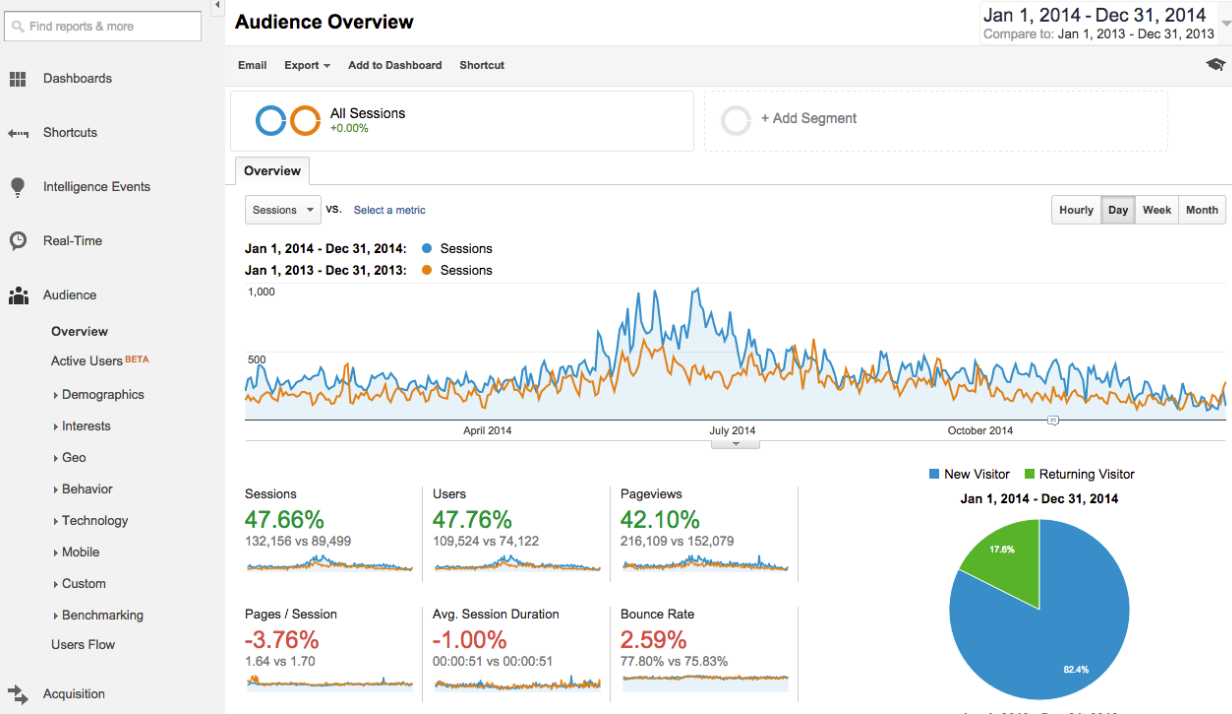
\includegraphics[scale=0.8]{ga.png}  
  \caption{Google Analitics}
	\label{fig:ga}
\end{figure}


Преимущества:
\begin{itemize}
\item способность отслеживать статистику переходов на сайт;
\item способность классифицировать посетителей, что позволяет разрабатывать новые страницы сайта более эффективно с учетом потребностей целевой аудитории;
\item способность отслеживать исходящие ссылки, используемые при продвижении сайта, также необходимые для дальнейшей раскрутки сайта;
\item способность отслеживать ссылки, которые скачивают больше всего;
\item способность отслеживать адреса электронной почты по кликам;
\item практически все коммерческие транзакции прослеживаются при помощи Google Analytics;
\item можно отключить статистику посещений тех, кто обслуживает сайт;
\item Сравнение статистики посещения сайта за разные периоды. Данная возможность идеальна для выявления эффективности работы новых страниц.
\end{itemize}


Недосатки:
\begin{itemize}
\item невозможно отследить трафик, если у пользователя отключены cookies;
\item Google Analytics не может повторно обработать данные, если потерян профиль с настроенными фильтрами;
\item настройка отчетов имеет ограниченное количество параметров;
\item количество отслеживаемых целей также ограничено (настоящее время Google Analytics отслеживает до четырех целей).
\end{itemize}

\subsection{CRM системы}
\label{sub:alternatives:crm}
Раньше CRM системы были доступны только для корпоративного сектора. Исключительно компании с развитой технологической инфраструктурой, огромным штатом сотрудников и достаточным бюджетом могли приобрести CRM систему для автоматизации работы отделов продаж, маркетинга и сервисного обслуживания клиентов.
Постепенно с тем, как увеличивалась скорость Интернет-подключения, появлялись облачные технологии и приобретали свою популярность SaaS решения (англ. software as a service — программное обеспечение как услуга), приобретение CRM систем становилось доступной опцией для любой компании.

Сегодня рынок CRM является динамичным и быстрорастущим. Облачные технологии позволяют легко внедрять CRM системы с нуля, без особых технических хлопот с развертыванием и по низкой стоимости. Далее приведены основные характеристики CRM систем, покупательские критерии, а также сравнения CRM решений от разных поставщиков. Конечно есть свои нюансы, и бизнесы должны полагаться на свои собственные требования при выборе оптимальной CRM системы. Далее рассмотрены базовые параметры, на которые следует обратить внимание при выборе CRM системы:
\begin{itemize}
\item варианты хостинга;
\item наличие мобильного клиента;
\item стоимость;
\item функционал для продаж;
\item функционал для маркетинга;
\item наличие сервисного модуля;
\item возможности хранения документов на дисковых пространствах CRM системы;
\item модуль отчетности.
\end{itemize}

Далее приведен обзор следующих CRM систем: SugarCRM, Salesforce.com, Microsoft Dynamics CRM и Zoho ~\cite{crms}.


\subsubsection{SugarCRM }
\label{sub:alternatives:crm:sugar}
SugarCRM (рисунок~\ref{fig:sugar}) предлагает систему для поддержки процессов продаж, маркетинга и сервисного обслуживания. Стоимость лицензии начинается от \$35 за пользователя в месяц в рамках редакции Professional с возможностью развертывания решения на серверах предприятия и до \$150 за пользователя в месяц за редакцию Ultimate. В рамках подписки на все редакции предоставляется мобильный клиент, а размеры хранилища документов варьируются от 15 Гб в редакции Professional до 250 ГБ – в Ultimate ~\cite{sugar}.

\begin{figure}[h]
\centering
  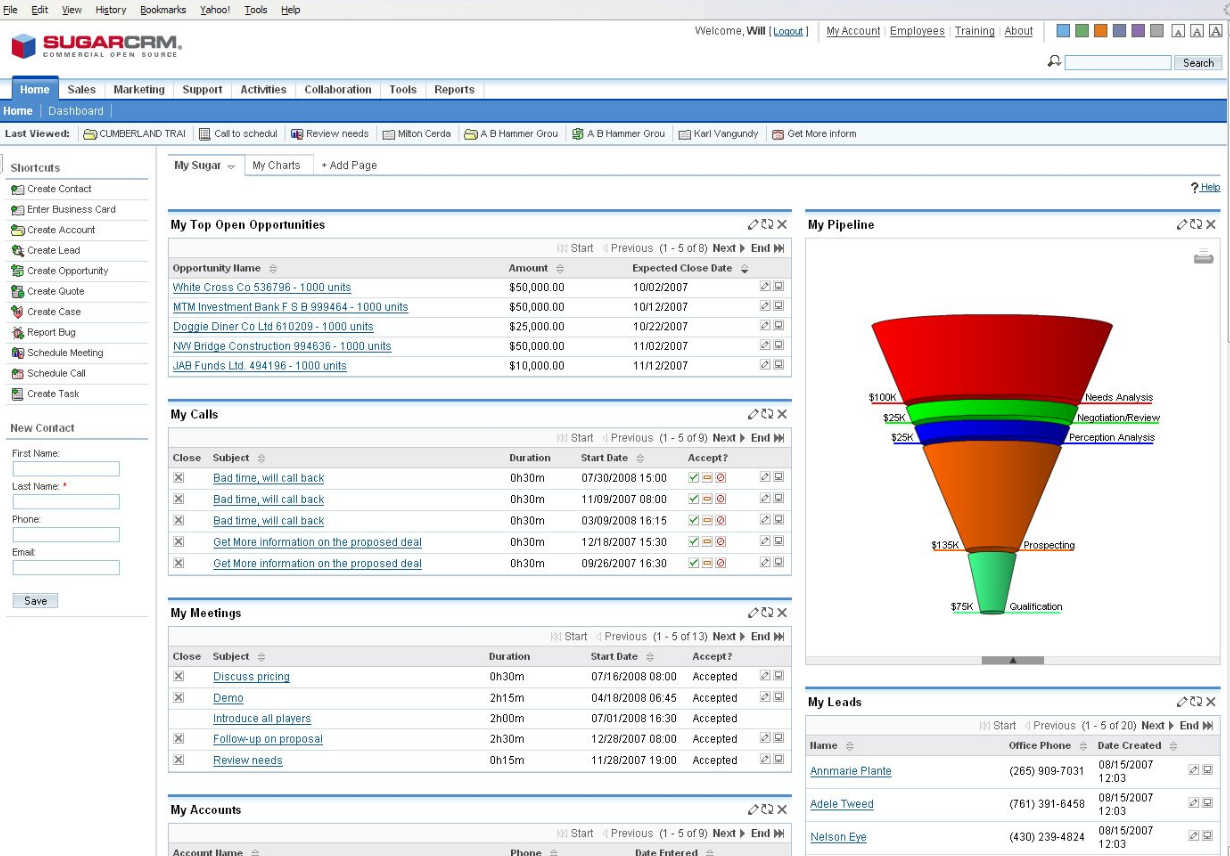
\includegraphics[scale=0.7]{sugarCRM.png}  
  \caption{SugarCRM}
  \label{fig:sugar}
\end{figure}

Основные функциональные возможности SugarCRM:
\begin{itemize}
\item Workflow или автоматические процессы. Позволяет автоматически настраивать события и следить за их выполнением. В продажах этот механизм особенно важен: позволяет создавать новые продажи с различным бюджетом, контролировать пребывание продажи на конкретной стадии и многое другое.
\item Интеграция с SMS. Как и интеграция с социальными сетями стала неотъемлемой частью работы компании, SMS сервисы стали важными каналами коммуникации с клиентами и предоставления сервиса последним. Возможность интегрировать CRM систему и сервис SMS сообщений является важным преимуществом.
\item Функция Web-to-lead. CRM система Sugar также позволяет собирать клиентские данные с веб-сайта компании и автоматически аккумулировать эти данные в CRM системе.
\end{itemize}

Преимущества: 
\begin{itemize}
\item SugarCRM имеет открытый исходный код, поэтому система достаточно гибкая и масштабируемая с возможностью расширения под потребности бизнеса;
\item систему можно достаточно легко настраивать под предпочтения бизнес пользователей.
\end{itemize}

Недостатки: 
\begin{itemize}
\item чтобы пользоваться SugarCRM нужны определенные знания и компетенции, на обучение требуется время.
\end{itemize}



\subsubsection{Salesforce CRM }
\label{sub:alternatives:crm:sf}
Salesforce CRM (рисунок~\ref{fig:sf}) лидирует в сегменте облачных CRM систем уже на протяжении многих лет. Salesforce.com предлагает CRM систему Sales Cloud, которая поставляется в пяти редакциях, начиная с базовой редакции Contact Manager стоимость лицензии которой начинается от \$5 за пользователя в месяц. Наиболее популярная редакция, которая наилучшим образом удовлетворяет бизнес потребности большинства компаний является Enterprise. Ее стоимость составляет \$125 за пользователя в месяц; редакция поставляется с функционалом по ведению и управлению продажами, управлению процессами lead менеджмента, настраиваемыми рабочими столами (dashboard), workflow и возможностями интеграции через API. 

Основные функциональные возможности Salesforce.com:
\begin{itemize}
\item Синхронизация с Outlook. Данные из CRM системы Salesforce автоматически синхронизируются с Outlook, включая контакты, календарь и многое другое.
\item Настраиваемые процессы продаж. Можно адаптировать процессы продаж под модель организации компании. Это играет ключевую роль при выборе CRM системы, потому что продавцам очень важно использовать технологию, в которой доступны не только стандартные процессы.
\item Функция Web-to-lead. Эта функция позволяет компаниям собирать информацию со своих сайтов и генерировать ее внутри CRM системы Salesforce, на основе этих данных создавать лиды.
\item Мобильный доступ в режиме offline. Очень важная опция для полевых продавцов, которые могут вводить данные в CRM систему с мобильного в автономном режиме и позже синхронизировать эти данные в CRM при возобновлении подключения к Интернет.
\item Интеграция через web-сервисы API. Эта опция позволяет CRM системе Salesforce синхронизироваться с другими backend офисными системами, такими как ERP, системами финансового учета, а также дает возможность компаниям расширять функциональность и интегрировать систему с другими технологиями.
\end{itemize}


\begin{figure}[h]
\centering
  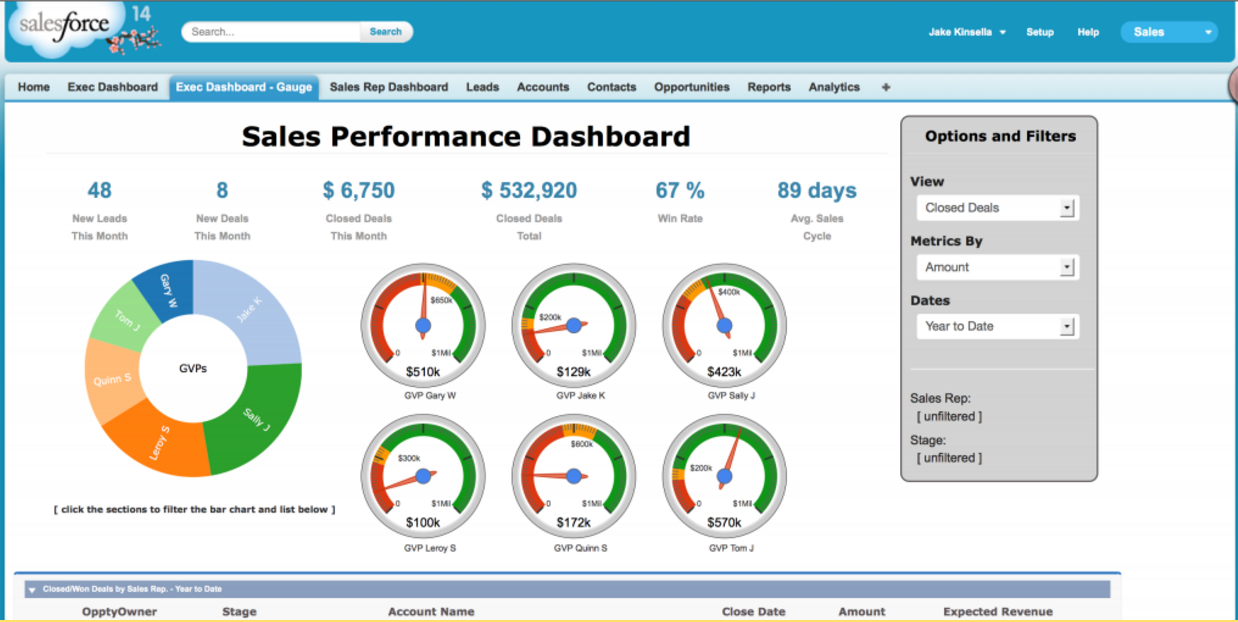
\includegraphics[scale=0.7]{sf.png}  
  \caption{Salesforce CRM}
	\label{fig:sf}
\end{figure}

Преимущества: 
\begin{itemize}
\item гибкость системы, наличие ключевых CRM функций, в том числе визуализация воронки продаж в режиме реального времени;
\item мобильный клиент для всех редакций системы;
\item возможная интеграция с инструментами работы с данными от третьих производителей, такими как Data.com, Twitter, LinkedIn, YouTube и Klout, увеличит производительность работы на всех этапах цикла продажи, от потенциального клиента до клиента.
\end{itemize}

Недостатки: 
\begin{itemize}
\item только облачный вариант развертывания, что ставит под вопрос безопасность клиентских данных для некоторых компаний;
\item стоимость редакций Professional и Enterprise дороже, чем у большинства других игроков рынка.
\end{itemize}


\subsubsection{Microsoft Dynamics CRM }
\label{sub:alternatives:crm:msDM}
Microsoft Dynamics CRM (рисунок~\ref{fig:msDM}) поздно появилась на рынке CRM, и ранние редакции Microsoft CRM не имели большого спроса среди пользователей.  Стоимость этой редакции начинается от \$65 за пользователя в месяц. Dynamics CRM – это технология с полным набором различных функций -- от управления лидами и до заключения продажи, поэтому с помощью Dynamics CRM можно выстраивать полноценные отношения с клиентами. CRM система интегрируется с другими инструментами от Microsoft – программным пакетом Office и Office 365 -- для ведения email коммуникаций, анализа данных и управления документами – однако это все за дополнительную плату ~\cite{msdyn}.


% \FloatBarrier
\begin{figure}[h]
\centering
  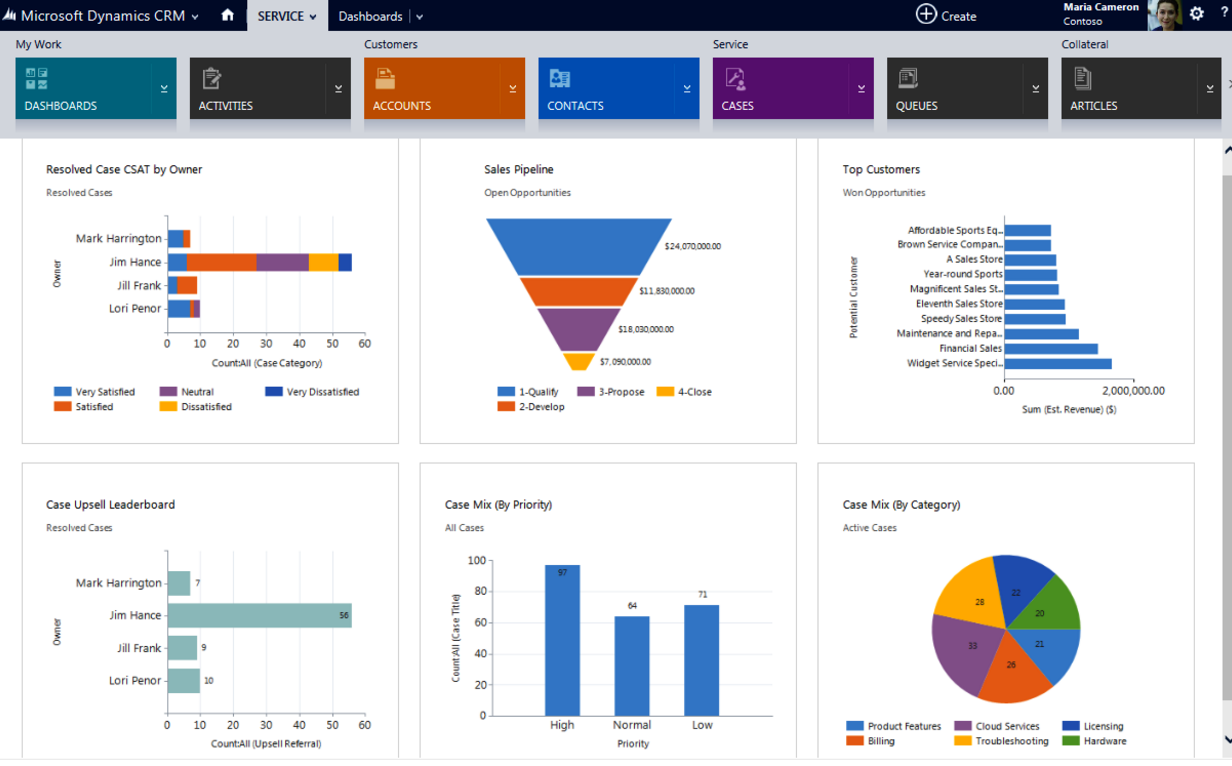
\includegraphics[scale=0.7]{microsoftDM.png}  
  \caption{Microsoft Dynamics CRM}
  \label{fig:msDM}
\end{figure}

Основные функциональные возможности Dynamics CRM:
\begin{itemize}
\item интеграция с Microsoft Office;
\item Настраиваемые отчеты и рабочие столы. Есть возможность генерировать кастомизированные отчеты для руководства.
\item Механизм workflow для настройки бизнес процессов. Можно планировать и оптимизировать бизнес-процессы в CRM системе Dynamics с помощью данного инструмента.
\item Интеграция через web-сервисы. Microsoft синхронизируется с другими backend офисными системами, такими как ERP системы, системы финансового учета и др.
\item Мобильный доступ. Microsoft разработала систему Dynamics с доступной мобильной версией.
\item Настраиваемые сущности. Эта функция позволяет третьим производителям дорабатывать функционал готовой CRM системы. Например, настроенная сущность <<Проект>> может быть создана для управления отношениями между контактами и контрагентами с поддержкой функционала существующих сущностей системы.
\item Соглашение о качестве предоставляемых услуг. Microsoft подписывает соглашение о качестве предоставляемых услуг, которое обеспечивает компаниям безопасность клиентских данных, а также страхует их от потери данных и других потенциальных угроз.
\end{itemize}

Преимущества: 
\begin{itemize}
\item Microsoft обладает богатым функционалом для увеличения лидов до продажи или сервисного обращения;
\item Microsoft хорошо интегрируется с другими продуктами для повышения производительности бизнеса, такими как Office и Office 365.
\end{itemize}

Недостатки: 
\begin{itemize}
\item решение Microsoft CRM стоит очень дорого;
\item известно больше как преемник тенденций, а не новатор.
\end{itemize}


\subsubsection{Zoho CRM }
\label{sub:alternatives:crm:zoho}
Zoho CRM (рисунок~\ref{fig:zoho}) предлагает различные онлайн продукты и облачные технологии; CRM система – одна из них. Стоимость владения системой довольно низкая; система поставляется на бесплатной основе, если количество пользователей не превышает 3 единицы, и может послужить хорошей отправной точкой для представителей малого бизнеса. На таких условиях предоставляется базовый функционал управления лидами, продажами, контрагентами и контактами ~\cite{zoho}. 

\pagebreak
\begin{figure}[h]
\centering
  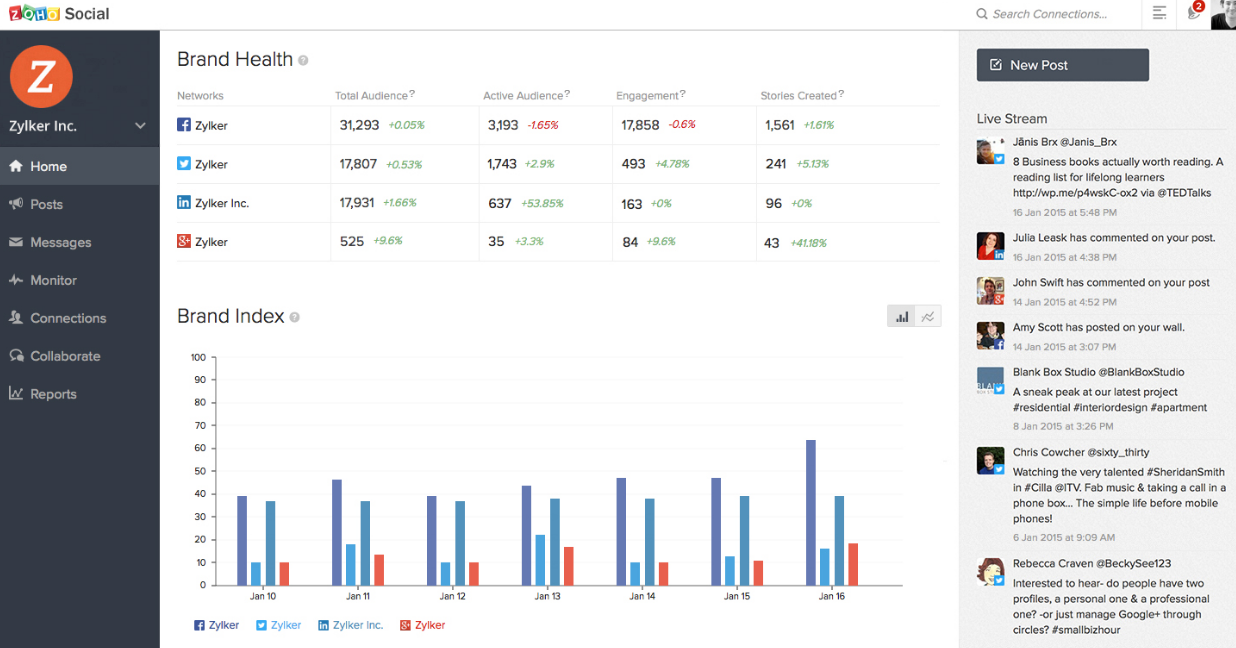
\includegraphics[scale=0.7]{zoho.png}  
  \caption{Zoho CRM}
  \label{fig:zoho}
\end{figure}

Основные функциональные возможности Zoho:
\begin{itemize}
\item Функция Web to lead, case формы. Пользователи могут собирать данные из форм непосредственно в CRM систему Zoho.
\item Настраиваемые рабочие столы. На рабочий стол пользователи могут выводить нужную им информацию для оперативной работы.
\item Автоматизация маркетинга. Инструмент автоматизации маркетинга автоматически сегментирует целевую аудиторию компании для точечного обращения и позволяет измерять затраченные усилия.
\item Интеграция с Twitter и Facebook. Увеличение роли социальных сетей в улучшении клиентского опыта. Необходимость отслеживать поведения клиентов в социальных медиа, а также потребность в повышении эффективности маркетинга, делают интеграцию с социальными платформами обязательным элементом для CRM систем.
\end{itemize}

Преимущества: 
\begin{itemize}
\item сбор данные веб-форм сайта непосредственно в СRM систему;
\item можно попробовать CRM систему перед тем, как приобретать ее;
\item Zoho является достойным продуктом и по стоимости уступает большинству.
\end{itemize}

Недостатки: 
\begin{itemize}
\item бесплатная редакция хороша в качестве пробы, но у нее есть жесткое ограничение по количеству данных, которые могут хранится в системе.
\end{itemize}


\subsection{FullContact}
\label{sub:alternatives:fullcontact}
FullContact (рисунок~\ref{fig:fc}) позволяет легко искать информацию о пользователе по email, телефонном номере или по имени аккаунта в твитере. Он позволяет найти всю публичную информацию из доступных социальных сетей, фотографий, географического положения, карьере и около 100 других различных данных о пользователе ~\cite{fullcontact}. 


\begin{figure}[h]
\centering
  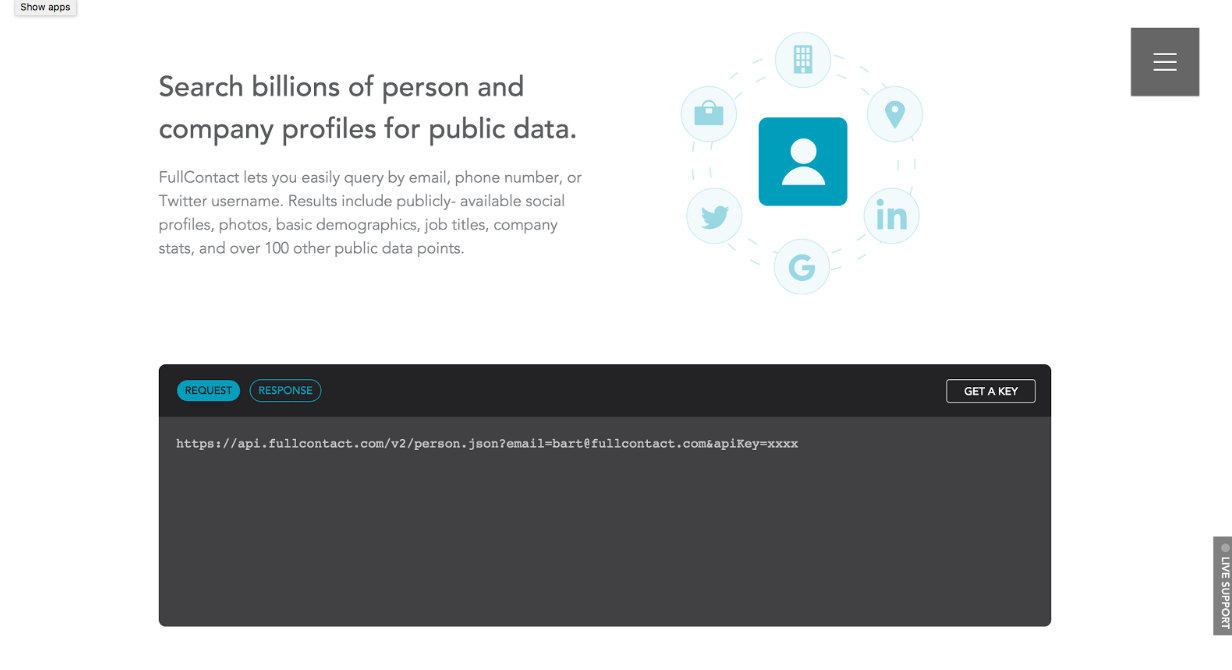
\includegraphics[scale=0.8]{fullContact.png}  
  \caption{FullContact}
	\label{fig:fc}
\end{figure}

Преимущества:
\begin{itemize}
\item предоставляет всевозможную публичную информацию об интересующих объектах;
\item простая интеграция;
\item оплата зависит от количества произведенных запросов.
\end{itemize}
Недостатки:
\begin{itemize}
\item является всего лишь сервисом по предоставлению публичной информации;
\item оплата зависит от количества произведенных запросов.
\end{itemize}

\pagebreak
\subsection{Постановка задачи}
\label{sub:alternatives:task}
Таким образом, проанализировав существующие готовые решения, было решено разработать программное средство предоставляющие возможность объединить их преимущества вместе и сынтегрировать их все в одну платформу. Оно должно обладать следующими свойствами:

\begin{itemize}
\item легко интегрироваться с другими программными средствами и горизонтально масштабироваться; 
\item иметь интеграцию с онлайн чатом CRM Salesforce;
\item иметь функционал трекинга событий произведенных пользователем на сайте;
\item иметь панель администратора, включающую в себя: просмотр статистики по пользователям как для выбранного периода времени, так и в режиме онлайн, возможность добавления администраторами и менеджерами новых событий в любое время;
\item интеграция с FullContacts для собирания публичной информации о пользователе из доступных социальных сетей, фотографий, географического положения, карьере и других различных данных о пользователе;
\item отказоустойчивость.
\end{itemize}


% Глава ? Модели, положенные в основу разрабатываемого программного средства
\section{Модели, положенные в основу разрабатываемого программного средства}
\label{sec:models:intro}


\subsection{Функциональная модель программного средства}
\label{sub:models:func_model}

Для представления функциональной модели была выбрана диаграмма вариантов использования UML, которая отражает отношения между актерами и прецедентами и позволяет описать систему на концептуальном уровне.

\begin{figure}[ht]
\centering
  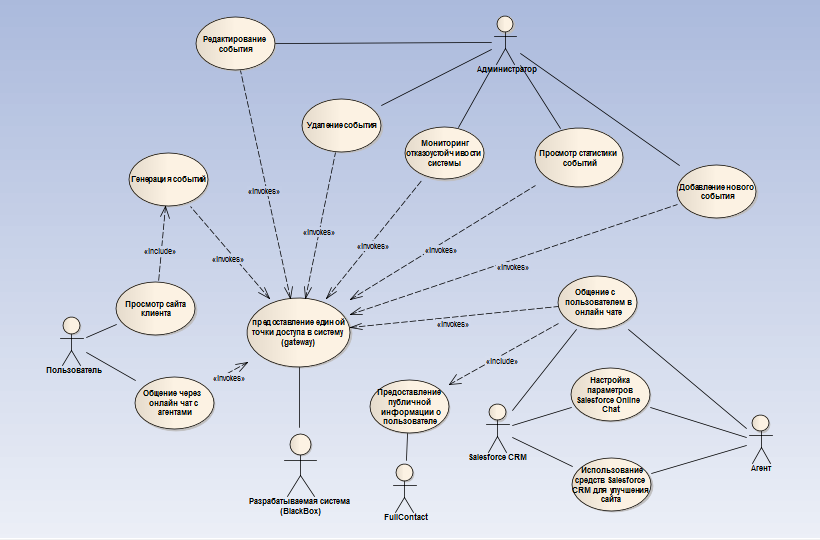
\includegraphics[scale=0.6]{uc-actors.png}  
  \caption{Функциональная модель}
	\label{fig:uc-actors}
\end{figure} 

Функциональная модель представлена на (рисунке~\ref{fig:uc-actors}).

На основании представленной диаграммы функциональной модели можно сделать вывод, что в системе будет существовать как минимум 6 актеров:
\begin{itemize}
\item пользователь;
\item агент;
\item администратор;
\item Salesforce CRM;
\item FullContact;
\item разрабатываемая система (BlackBox).
\end{itemize}
 
Рассмотрим каждого актера с его функциями более подробно.


Пользователь -- у пользователя в данной системе только две функции: он просматривает сайт (и тем самым генерирует события) и общается в онлайн чате с агентом.

Агент -- агент работает в Salesforce CRM. Он настраивает параметры для Salesforce Online Chat для отдельных страниц сайта, со своими особыми правилами появления чата, непосредственно общается с пользователем сайта, чтобы помочь последним и использует средства Salesforce CRM для улучшения сайта в результате диалога с пользователем.

Администратор -- настраивает систему отслеживания событий (добавляет/удаляет/редактирует события), следит и просматривает статистики происходящих событий для того чтобы понять как можно улучшить сайт. Также администратор наблюдает за отказоустойчивостью системы, чтобы в случае непредвиденных сбоев (потеря сети или интернета, выхода из строя серверов) быть готовым среагировать на возникшую проблему.

Salesforce CRM -- внешняя система, благодаря интеграции с которой, возникает возможность многофункционального онлайн чата с пользователем, а также возможность использования информации от него.

FullContact -- внешняя система, благодаря интеграции с которой, можно получить доступную публичную информацию о пользователе.

Разрабатываемая система (BlackBox) -- система, которая позволит всем перечисленным выше актерам выполнить свои функции. Она будет подробно рассмотрена в разделе ~\ref{sub:design:ps}  (рисунок~\ref{fig:uc-services}).


\subsection{Спецификация функциональных требований}
\label{sub:models:func_req}

Таким образом основной целью данного проекта является создание программного средства, позволяющего легко внедрять и использовать другие внешние сервисы и интегрировать их друг с другом.

В ходе разработки будут реализованы следующие возможности:
\begin{itemize}
\item интеграция с онлайн чатом CRM Salesforce;
\item создание системы отслеживания событий (event tracking system);
\item возможность настраивать онлайн чат с агентами определенных типов в зависимости от страницы сайта, на которой он должен появляться;
\item возможность настраивать онлайн чат так, чтобы сначала пользователь говорил с агентом одного типа (например обслуживающим лицом), а потом его, по результату разговора, можно было перенаправить на агента другого типа (например продавца);
\item возможность отслеживать процесс перехода состояний онлайн чата с помощью системы отслеживания событий;
\item возможность в панели администратора настраивать модели событий (создания/редактирования/удаления), которые сможет обрабатывать система отслеживания событий; 
\item возможность отслеживать действия пользователя на сайте с помощью системы отслеживания событий;
\item возможность в панели администратора просмотра (online/offline) статистики происходящих событий;
\item создание сервиса для нахождения публичной информации о пользователе с помощью интеграции с FullContact;
\end{itemize}

\subsection{Спецификация нефункциональных требованиями}
\label{sub:models:func_non_req}

Программное средство должно обладать следующими нефункциональными требованиями:
\begin{itemize}
\item работать в любом современном браузере(Chrome 40+, IE9+, Safari 7.7+, Firefox 3.6+);
\item интегрироваться с помощью js сниппета;
\item быть легковесным  и иметь как можно меньше накладных расходов для систем клиентов (подгружаемые скрипты должны быть < 10kb);
\item иметь интуитивно понятный интерфейс для просмотра статистик, чтобы новый пользователь мог его освоить за 2-3 дня;
\item иметь возможность легко включаться, выключаться и удаляться из систем клиентов;
\item иметь задержку не более 200ms при обращении к сервисам;
\item иметь возможность горизонтально масштабировать отдельные компоненты системы;
\item иметь возможность просмотра состояний отдельных компонентов системы;
\item иметь возможность работать с большим объемом поступающих входных данных (гигабайтами в день).
\end{itemize}


% Глава ? Проектирование программного средства
\section{Проектирование программного средства}
\label{sec:design:intro}

\subsection{Архитектура микросервисов}
\label{sub:design:micro}

Так как разрабатываемая система должна быть легко расширяема для нового функционала и интеграции, быть высокопроизводительной, отказоустойчивой и приспособлена к работе с большим количеством поступающих данных, то в качестве основной модели положенной в разработку данного программного средства была выбрана микросервисная архитектура.

Архитектурный стиль микросервисов -- это подход, при котором единое приложение строится как набор небольших сервисов, каждый из которых работает в собственном процессе и коммуницирует с остальными используя легковесные механизмы, как правило HTTP. 

На рисунке~\ref{fig:micro-vs-mono} представлено сравнение микросервисной архитектуры с монолитной.

\begin{figure}[ht]
\centering
  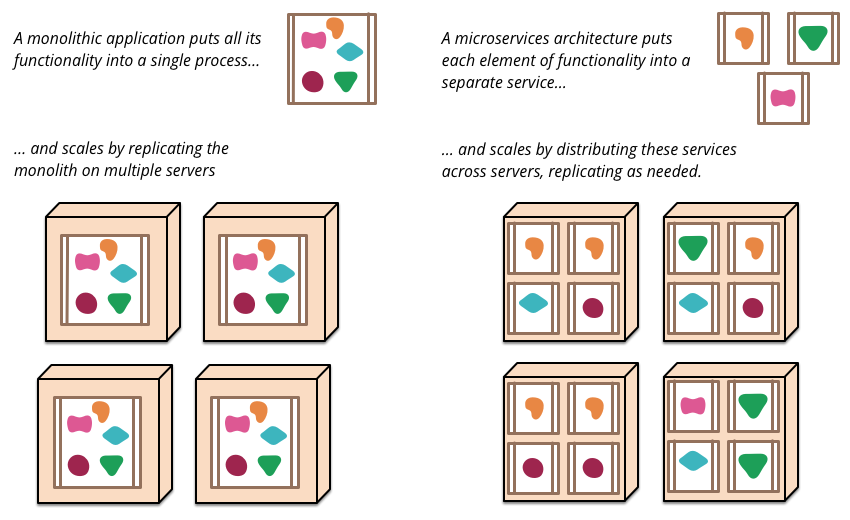
\includegraphics[scale=0.5]{micro-vs-mono.png}  
  \caption{Сравнение микросервисной архитектуры с монолитной}
	\label{fig:micro-vs-mono}
\end{figure} 


Эти сервисы построены вокруг бизнес-потребностей и развертываются независимо с использованием полностью автоматизированной среды. Существует абсолютный минимум централизованного управления этими сервисами. Сами по себе эти сервисы могут быть написаны на разных языках и использовать разные технологии хранения данных. Таким образом система получается легко расширяема для нового функционала и интеграций.

Благодаря тому, что в микросервисной архитектуре легко горизонтально масштабировать отдельные сервисы, её можно приспосабливать к работе с большим количеством поступающих входных данных и добиться высокой производительности.

В то время как монолитные приложения склонны к использованию единственной БД для хранения данных, компании часто предпочитают использовать единую БД для целого набора приложений. Такие решения, как правило, вызваны моделью лицензирования баз данных. Микросервисы предпочитают давать возможность каждому сервису управлять собственной базой данных: как создавать отдельные экземпляры общей для компании СУБД, так и использовать нестандартные виды баз данных. Этот подход называется Polyglot Persistence ~\cite{micro}.

На рисунке~\ref{fig:micro-db} представлено сравнение хранения данных микросервисной архитектуры с монолитной.

\begin{figure}[ht]
\centering
  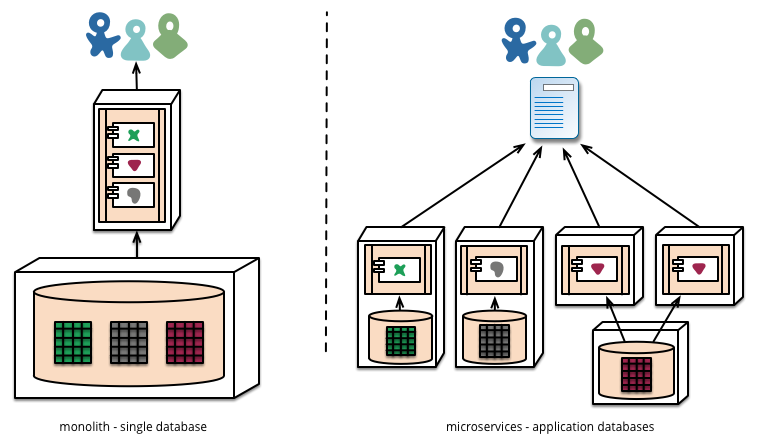
\includegraphics[scale=0.5]{micro-db.png}  
  \caption{Сравнение хранения данных в микросервисной архитектуре с монолитной}
	\label{fig:micro-db}
\end{figure} 



Микросервисная архитектура делает большой акцент на мониторинге приложения в режиме реального времени, проверке как технических элементов (например, как много запросов в секунду получает база данных), так и бизнес-метрик (например, как много заказов в минуту получает приложение). Семантический мониторинг может предоставить систему раннего предупреждения проблемных ситуаций, позволяя команде разработке подключиться к исследованию проблемы на самых ранних стадиях. Таким образом, можно добиваться отказоустойчивости ~\cite{micro}.

Микросервисная архитектура позволяет упростить и ускорить процесс релиза, так как не требует пересборки и развертывания всего приложения, как в случае с монолитным приложением. Вместо этого нужно развернуть (redeploy) только те сервисы, которые изменились.



\subsection{Архитектура программного средства}
\label{sub:design:ps}


Диаграмма взаимодействия сервисов разрабатываемого программного средства представлена на (рисунок~\ref{fig:uc-services}). Актером в данном случае является отдельный микросервис системы, имеющий свою роль в системе. Прецедент – эллипс с надписью, обозначающие какие функции предоставляет тот или иной микросервис.

\begin{figure}[ht]
\centering
  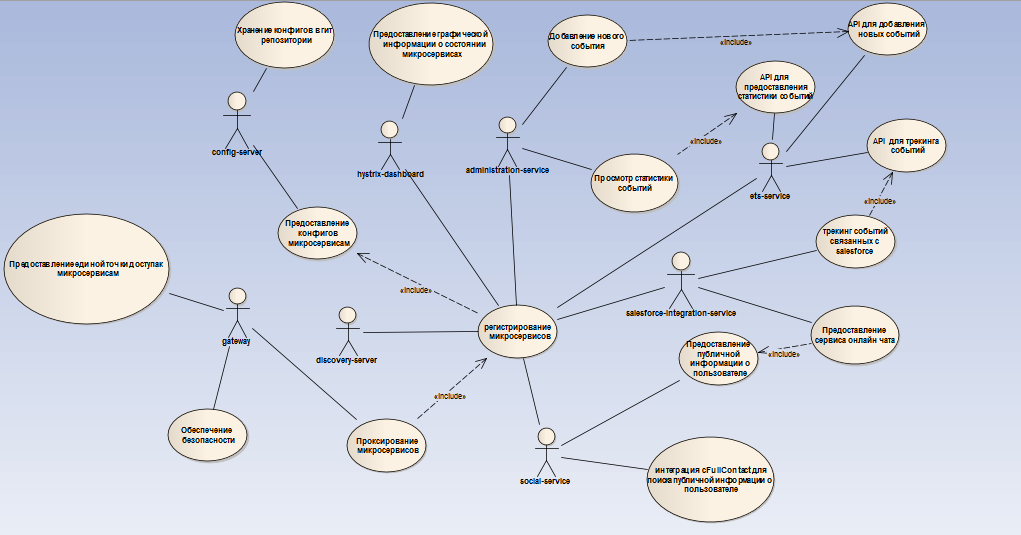
\includegraphics[scale=0.6]{uc-services.png}  
  \caption{Диаграмма взаимодействия сервисов}
	\label{fig:uc-services}
\end{figure} 

На основании представленной диаграммы взаимодействия сервисов можно сделать вывод, что в системе будет существовать семь микросервисов:
\begin{itemize}
\item gateway;
\item config-server;
\item discovery-server;
\item administration-service;
\item salesforce-integration-service;
\item social-service;
\item ets-service.
\end{itemize}
 
Рассмотрим каждого актера с его функциями более подробно:

Discovery-server -- этот сервис позволяет микросервисам обнаруживать друг друга и общаться между собой.

Ets-service -- основной сервис в котором реализовано ядро с работой над событиями. Оно предоставляет API по созданию различных событий и их отслеживанию.

Administration-client -- сервис для администраторов и менеджеров в нем можно настраивать/редактировать/добавлять новые события, следить за их статистикой как за определенный период так и в режиме онлайн. 

Salesforce-integration -- сервис для интеграции с СRM системой Salesforce. Он также предоставляет онлайн чат для клиентов по различным условиям настраиваемым в Salesforce, а также записывает все необходимые события происходящие с CRM Salesforce c помощью ets-service.

Social-integration -- сервис для собирания публичной информации о пользователе, включает в себя интеграцию с FullContact который помогает в сборе информации из доступных социальных сетей, фотографий, географического положения, карьере и около 100 других различных данных о пользователе

Config-server -- это сервис для централизованного хранения конфигурации всех микросервисов в отдельном git репозитории ~\cite{cloud_config}.

Hystrix-dashboard -- это сервис предоставляет возможность графического мониторинга состояния всех микросервисов.

Gateway -- сервис предоставляющий централизованную точку доступа к другим сервисам, а также обеспечивает безопасность для всех остальных сервисов.

\subsubsection{Проектирование системы отслеживания событий}

Данное программное средство позволяет отслеживать события производящие на сайте пользователем. Для того, чтобы система сохраняла только нужные события, она должна позволять настраивать модели событий (удалять/добавлять/редактировать), которые будет способна обрабатывать. При сохранении события система проверяет находится ли подходящая модель для произошедшего события, и если таковая нашлась, сохраняет его.


На рисунке~\ref{fig:des-ets} приведена схема проектирования системы отслеживания событий.
\pagebreak
\begin{figure}[ht]
\centering
  \includegraphics[scale=0.6]{ets.png}  
  \caption{Схема проектирование системы отслеживания событий}
	\label{fig:des-ets}
\end{figure} 	


\subsubsection{Проектирование онлайн чата}
\label{sub:design:chat}

Для понимания того, какие проблемы могут возникнуть у пользователей на сайте будет разработан онлайн чат пользователя с агентом на основе Salesforce Online Chat. Salesforce Online Chat уже изначально включает в себя множество настроек, по которым пользователю будет показано приглашение посетить online chat с тем или иным типом агентом. Данное же программное средство включает в себя доработку возможности настраивать в salesfoce различные чаты для различных страниц сайта клиента. Также перед тем как будет установлен чат, система попробует найти публичную информацию о посетителе и предоставить её агенту, чтобы тот смог её использовать в своих целях (рисунок~\ref{fig:des-chat}).

На рисунке~\ref{fig:des-chat} приведена схема проектирования online chat с пользователем.


\begin{figure}[ht]
\centering
  \includegraphics[scale=0.6]{chat.png}  
  \caption{Схема проектирование Online Chat с пользователем}
	\label{fig:des-chat}
\end{figure} 




% Глава ? Разработка программного средства
\section{Разработка программного средства}
\label{sec:development:intro}

При построении данного дипломного проекта необходимо использовать некоторые основные компоненты от Spring Cloud и Netflix ОSS, позволяющие отдельно разворачивать микросервисы, а также наладить общение между ними без ручного управления. 

В итоге для создания нового экземпляра микросервиса и сбалансирования нагрузки нужно будет выполнить только несколько команд, чтобы начать использовать его без каких-либо ручных настроек.


\subsection{Язык программирования Java}
\label{sub:development:java}
В качестве основного языка программирования была выбрана Java, так как это статически компилируемый язык программирования, проверенные временем и имеющий огромное количество написанных под него библиотек и фреймворков. 

JVM оптимизирована для больших многоядерных машин, и она без проблем может управлять сотнями потоков, благодаря чему позволяет строить высокопроизводительные системы.

Существование JVM-подобных языков, таких как Groovy, Scala, Clojure является так же большим плюсом. Благодаря им, и тому что они полностью JVM совместимы, при разработки на java необязательно использовать только её, зачастую удобно совмещать несколько JVM-подобных языков программирования, чтобы в тех или иных случаях, получать преимущества получать преимущества того или иного языка.   

Благодаря фрэймворку Spring, и в частности его проекта Spring Cloud, java удобно использовать в построении микросервисной архитектуры, что является большим плюсом для данного программного средства, так как оно построено на ней. 

Также стоит отметить, что язык Java имеет превосходную среду разработки IntelliJ Idea, которая позволяет удобно и быстро разрабатывать программные средства.


\subsection{Spring Cloud и Netflix OSS}
\label{sub:development:netflix}

Spring Cloud ~\cite{spring_cloud} это достаточно новый продукт из экосистемы spring.io ~\cite{spring_site} с набором компонент которые удобно использовать для построения микросервисной архитектуры. В значительной степени Spring Cloud базируется на компонентах от Netflix OSS ~\cite{netflix_oss}.

Spring Cloud интегрирует компоненты Netflix в экосистему Spring используя автоматическую конфигурацию и конвенцию вместо обычной конфигурации подобно тому, как работает Spring Boot.

Приведенный ниже рисунок~\ref{fig:common-comp} отображает общие компоненты для реализации отдельных микросервисов ~\cite{tut_micros}:

\begin{figure}[ht]
\centering
  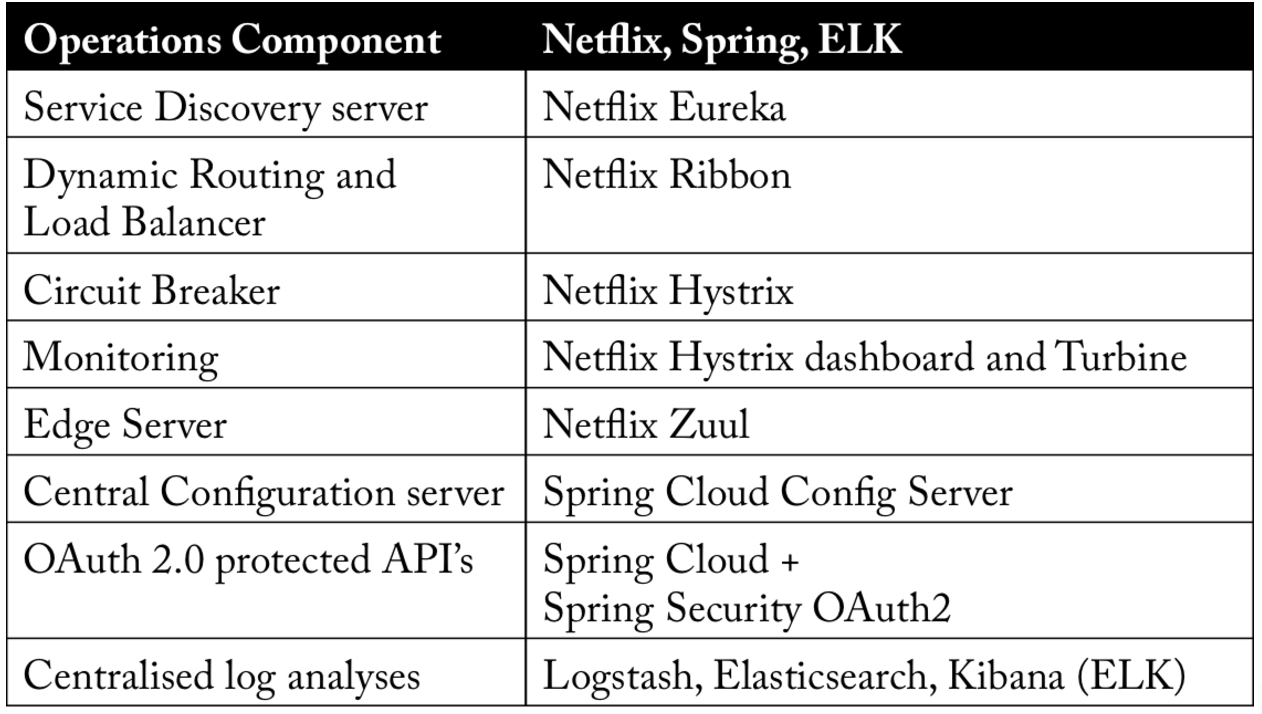
\includegraphics[scale=0.6]{common-comp.png}  
  \caption{Общие компоненты для реализации отдельных микросервисов}
	\label{fig:common-comp}
\end{figure} 



Netflix Eureka -- Service Discovery Server позволяет микросервисам регистрировать себя во время выполнения, так они появляются в микросервисной архитектуре ~\cite{eureka}.

Netflix Ribbon -- динамическая маршрутизация и балансировки нагрузки может быть использована для поиска экземпляра микросервиса для выполнения операции во время выполнения. Netflix Ribbon использует информацию, доступную в Eureka, чтобы найти соответствующие экземпляры служб. Если более чем один экземпляр найден, Netflix Ribbon будет применяться для балансировки нагрузки, чтобы распределить запросы по имеющимся экземплярам. Netflix Ribbon не является отдельным сервисом, но вместо этого используется в качестве встроенного компонента в других микросервисах ~\cite{ribbon}.

Netflix Zuul -- Edge Server Zuul это gateway с внешним миром, он не допускает каким-либо несанкционированным внешним запросам пройти в систему.  Edge Server также обеспечивает хорошо известную точку входа к какому-либо микросервису в микросервисной архитектуре. Использование динамически выделенных портов удобно для избежания конфликтов портов и для того чтобы свести к минимуму администрирование. Zuul использует Ribbon для поиска доступных микросервисов и маршрутов и отправляет внешний запрос к соответствующему экземпляру службы ~\cite{zuul}. 

Netflix Hystrix -- Circuit breaker Netflix Hystrix предоставляет возможности автоматического перенаправления вызова если произошли какие-либо проблемы с тем или иным микросервисом. Если микросервис не отвечает (например, из-за тайм-аута или ошибки связи), Hystrix может перенаправить вызов на внутренний метод запасного варианта. Если служба неоднократно не в состоянии ответить, Hystrix будет размыкать цепь вызывая внутренний аварийный метод, не пытаясь вызвать службу на каждом последующем вызове, пока сервис снова не станет доступным. Для того, чтобы определить, является ли сервис снова доступным Hystrix позволяют некоторым запросам попробовать достучатся до сервиса, даже если цепь была разорвана. Hystrix вводится как встроенный компонент в каждый отдельный микросервис ~\cite{hystrix}.

Netflix Hystrix dashboard and Netflix Turbine - специальное средство для мониторига статусов сервисов Hystrix. Оно обеспечивает графическое представление информации о состояниях всех сервисов, на основе информации, содержащейся в Eureka ~\cite{hystrix}. 

При реализации данного программного средства были построены следующие микросервисы:

Ets-service -- основной сервис в котором реализовано ядро с работой над событиями. Оно предоставляет API по созданию различных событий и их отслеживанию. 
Для хранения структуры различных событий используется реляционная база даны PostrgreSQL в которой описаны параметры событий, их типы, доступные значения, значения по умолчанию, наличие обязательности тех или иных полей и другая информации характеризующие то или иное событие.
Для отслеживания же самих событий используется NoSql база данных Mongo ~\cite{mongo}. Она лучше всего подходит для этой цели потому что, является быстрой бесструктурной документно-ориентированной базой данных, что позволят сохранять любые события созданные пользователем, а также изменять их в любое время
Отслеживание события происходит через предоставленное API. Перед тем как оно будет записано, происходит проверка на то что событие корректно, что осуществляется с помощью проверки его структуры. Для проверки же структуры все события подгружаются в Redis (высокопроизводительное не реляционное распределённое хранилище данных).


Administration-client -- сервис разработанный для администраторов и менеджеров в нем можно настраивать/редактировать/добавлять новые события, следить за их статистикой как за определенный период так и в режиме онлайн. 
Пользовательский интефейс разработан отдельно на Angular. 
Также стоит отметить что все API документируется с помощью Swagger, что позволяет frontend разработчикам сгенерировать нужное им API для обращения к построенной системе.


Salesforce-integration -- сервис, предоставляющий интеграцию с СRM системой Salesforce. В  котором также разработана интеграция  онлайн чата с клиентом, с сохранением соответствующие  события с помощью Ets-service.


Social-integration -- микросервис, разработанный для собирания публичной информации о пользователе, включающий в себя интеграцию с внешним сервисом публичной информации FullContact, который помогает в сборе информации из доступных социальных сетей, фотографий, географического положения, карьере и около 100 других различных данных о пользователе.


Discovery-server -- этот сервис позволяет микросервисам обнаруживать друг друга и общаться между собой (в данном случае использовалась Eureka).


Config-server -- это сервис, использующий Spring Cloud Config для централизованного хранения конфигурации всех микросервисов в отдельном git репозитории.

Во всех микросевисах использовался Hystrix для случаев, когда какой-то из них откажет. Данный же сервис предоставляет возможность графического мониторинга состояния всех микросервисов.


На рисунке~\ref{fig:save-event} изображен Hystrix Dashboard разрабатываемого программного средства.
\begin{figure}[ht]
\centering
  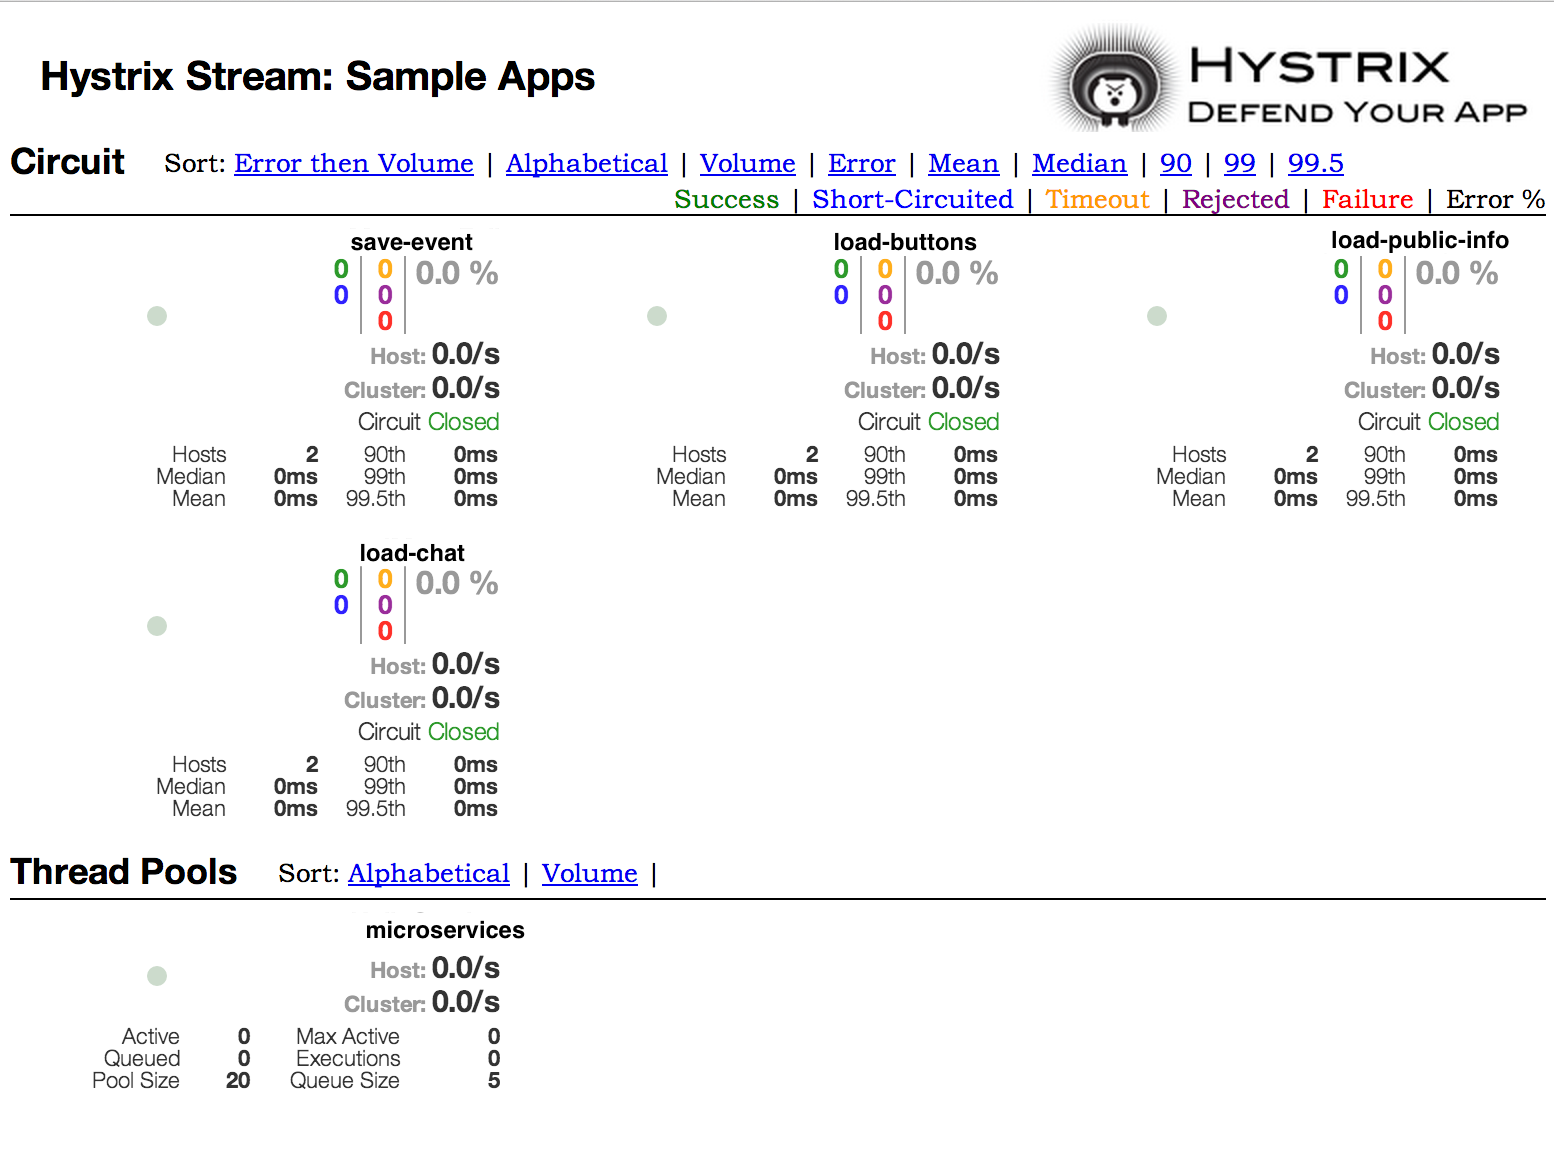
\includegraphics[scale=0.2]{hystrix.png}  
  \caption{Hystrix Dashboard программного средства}
  \label{fig:hystrix}
\end{figure} 



Gateway -- микросервис, использующий Netflix Zuul для предоставления централизованной точки доступа к микросервисам, также с помощью него и Spring Cloud Security настроена безопасность для всех микросервисов.


Для развертывания микросервисов используется docker и docker-compose.
С помощью них можно горизонтально масштабировать любой микросервис одной командой. 

Например одной командой docker-compose scale ets-service=5, поднимется 5 экземпляров микросервиса ets-service, и с помощью Ribbon другие микросервисы будут балансировать нагрузку по ним при обращении к сервису ets-service.


\subsection{Алгоритм сохранения события}
\label{sub:development:save_event}
Запросы на сохранение события, как и все остальные, сначала посылаются в микросервис gateway. В нем выполняется базовая аутентификация, которая проверяет, чтобы запросы обрабатывались только от клиентов, обладающих на это правами. Далее запрос отправляется с помощью Zuul Proxy в ets microservice, в котором находится логика обработки событий.

В самом же ets микросервисе событие о сохранении сразу же помещается в очередь сообщений RabbitMQ, таким образом все последующие действия выполняются асинхронно, и на стороне пользователя нету задержки, связанной с сохранением событий. Тем временем обработчик очереди событий RabbitMQ, постепенно обрабатывает все прилетевшие в него сообщения. Он же, в свою очередь, сначала пытается распознать к какому из типов моделей событие относится, то или иное сообщений, после чего, если тип найден, сохраняет событие его в MongoDB (рисунок~\ref{fig:save-event}).

После этого посылается ещё одно сообщение в RabbitMQ, теперь уже о результатах сохранения события, благодаря чему, все последующие действия опять выполняются асинхронно .
Обработчик сообщений предназначенный для обработки результатов сохранения в RabbitMQ, в свою очередь сохраняет результаты статистики и агрегирует их за последнее время по заданным критериям в системе. После чего эти данные отправляются в панель администратора, через вебсокеты, для того чтобы в ней можно было следить за происходящими событиями на сайте в режиме реального времени .%(рисунок~\ref{fig:save-event}). 

% На рисунке~\ref{fig:save-event} изображен алгоритм сохранения события.

\pagebreak
\begin{figure}[h]
\centering
  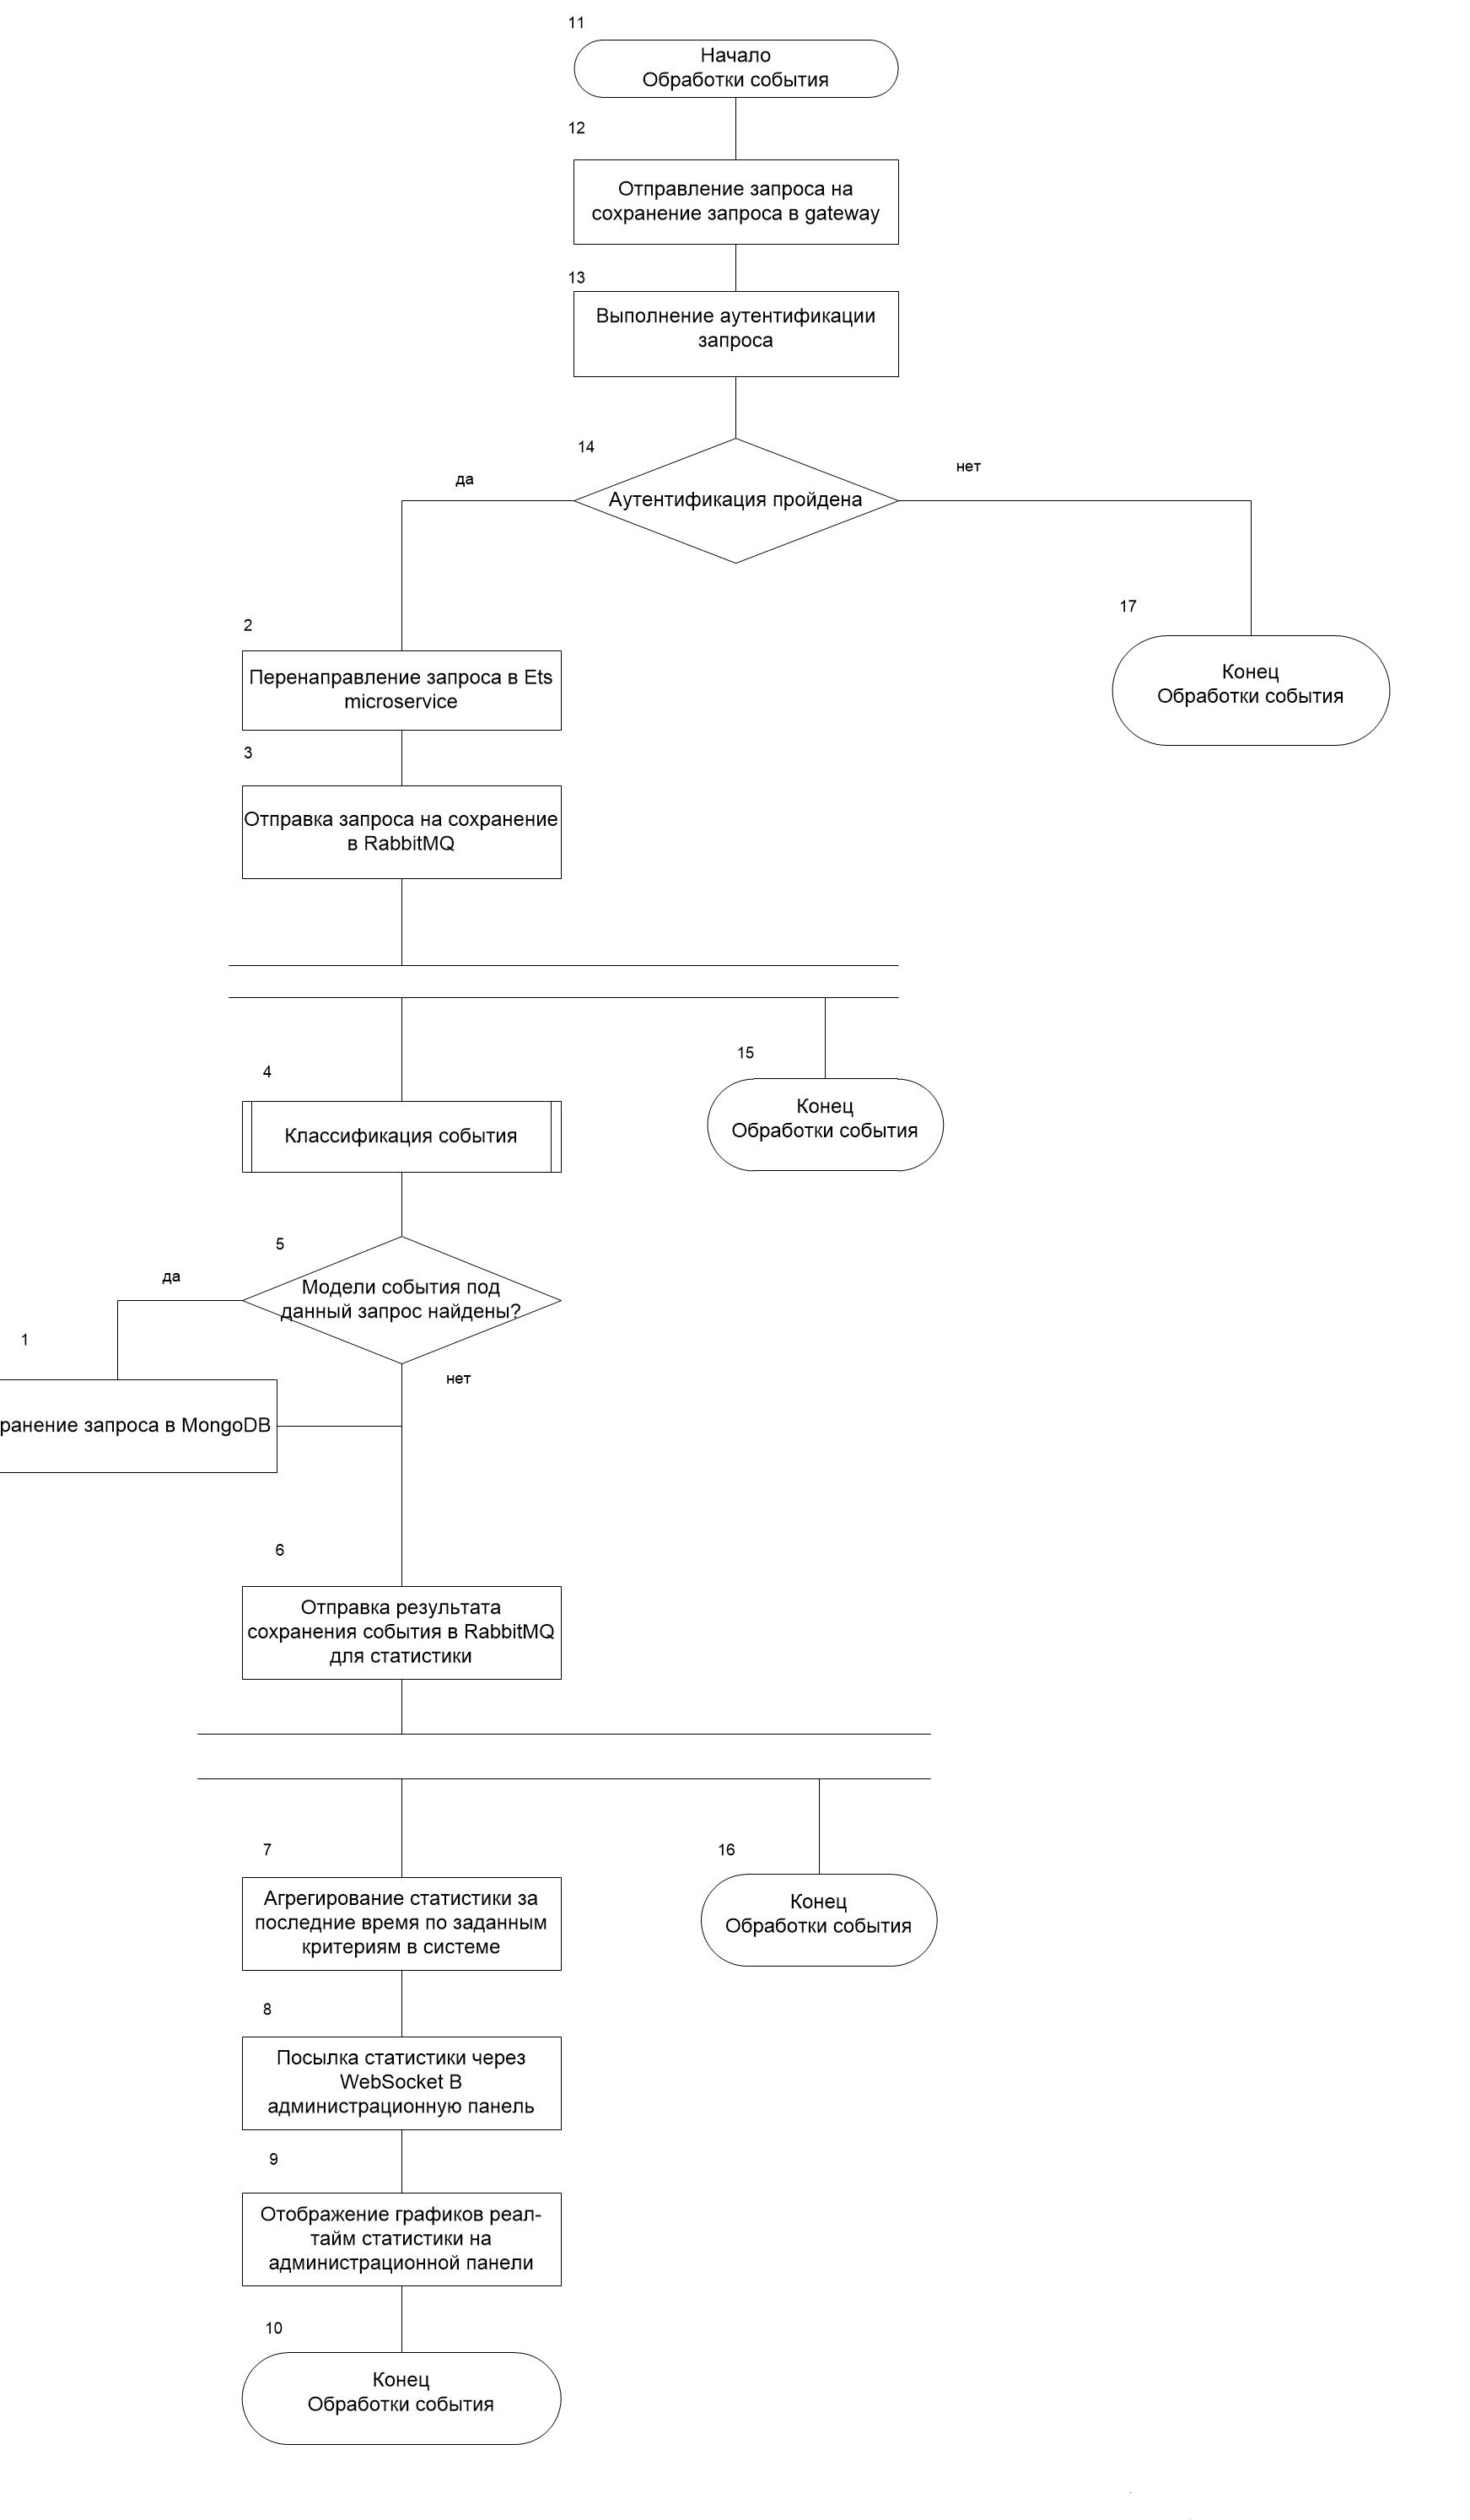
\includegraphics[scale=0.22]{save-event.png}  
  \caption{Алгоритм сохранения события}
  \label{fig:save-event}
\end{figure} 

\subsection{Алгоритм классификации событий}
\label{sub:development:klassific}
Все модели событий, которые принимает наша система, должны быть описаны в реляционной базе данных (в нашем случаем PostgreSQL) и их можно добавлять, удалять и изменять в любое время. 

Описание каждой модели включает в себя тип и набор полей, которые в неё входят. А каждое поле, в свою очередь, содержит информацию, к какому типу оно должно принадлежать(Date, Double, String, Long, List) и то, обязательно оно или нет (рисунок~\ref{fig:ets-domain}). 

% На рисунке~\ref{fig:ets-domain} приведена схема диаграмма классов модели событий.

\begin{figure}[h]
\centering
  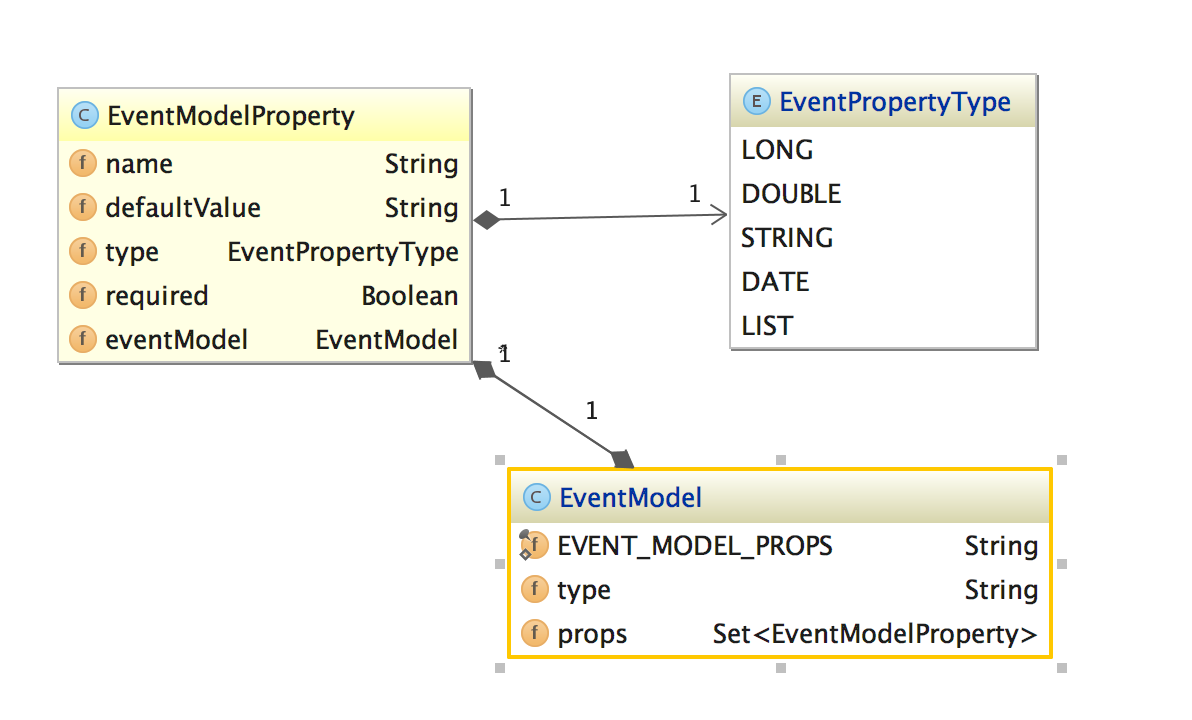
\includegraphics[scale=0.6]{ets-domain.png}  
  \caption{Диаграмма классов модели событий}
  \label{fig:ets-domain}
\end{figure} 


Алгоритм классификации событий определяет, к каким моделям событий можно соотнести пришедшее на вход событие, чтобы тип совпадал и все валидации проходили.
Первое что нужно алгоритму, это все модели данных, но так как все время обращаться в реляционную базу за ними было бы очень дорого и неэффективно, все модели подгружаются в in memory базу Redis ~\cite{redis}. Для того, чтобы данные в ней были все время актуальны, на ней настроен TTL, и поэтому через n-ое время все модели событий обновляются и всё время являются актуальными.

Сначала алгоритм ищет все модели событий у которых тип соответствует полю типа входного события, далее он идет по всем полям модели события, и проверяет, что пришедшее событие подходит под его модель: проверяет все обязательные поля и типы полей. Таким образом данный алгоритм находит все модели которые подходят для пришедшего события, а также валидирует их (рисунок~\ref{fig:klassification-event}).

% На рисунке~\ref{fig:klassification-event} приведена схема алгоритма классификации события.

\pagebreak
\begin{figure}[h]
\centering
  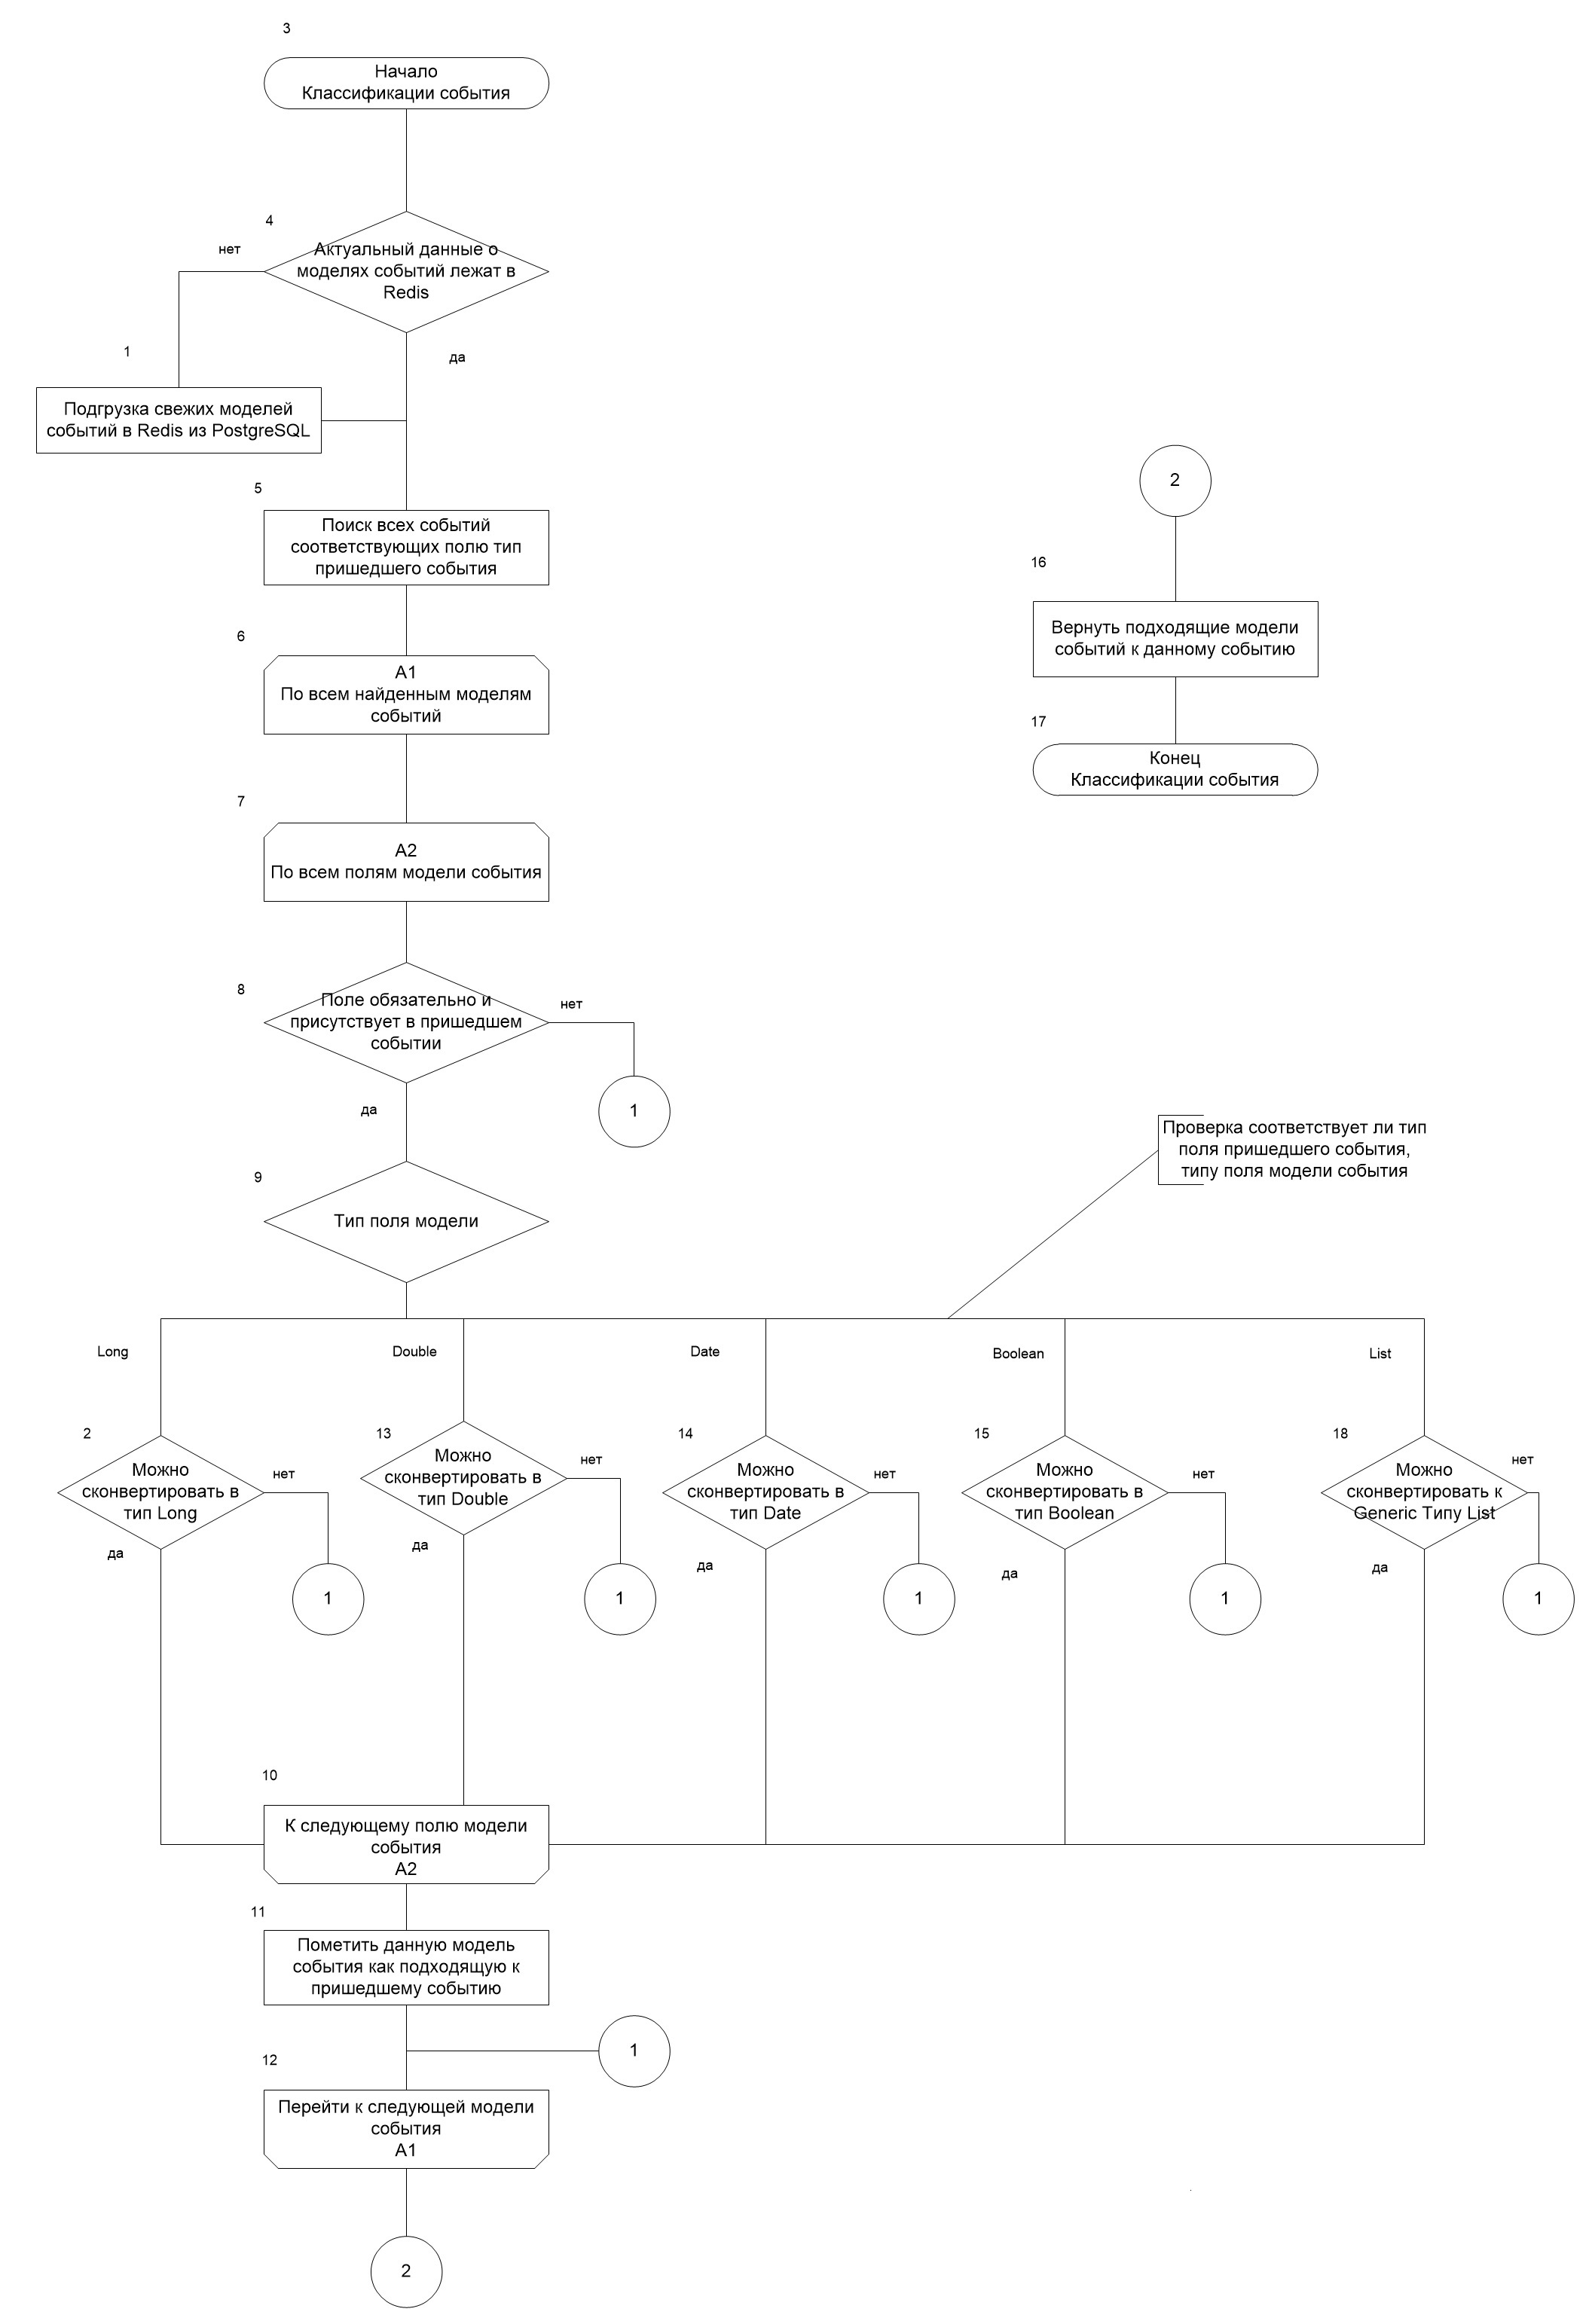
\includegraphics[scale=0.22]{klassification-event.jpg}  
  \caption{Алгоритм классификации события}
  \label{fig:klassification-event}
\end{figure} 



\subsection{Схема интеграции с онлайн чатом Salesforce}
\label{sub:development:chat}
Рассмотрим схему алгоритма интеграции с онлайн-чатом Salesforce ~\cite{live_agent}. 

Для интеграции c онлайн чатом Salesforce нужны стандартные объекты Salesforce, такие как LiveChatButton, DeploymentID и OrganizationID. Они включают в себя большое количество опций прямо из коробки Salesforce. Их описание можно найти в соответсвующей документации по SF. Отметим только, что LiveChatButton связывается с DeploymentID, и SF при подгрузке пытается подгрузить все LiveChatButton по соответствующим условиям, описанным в SF. Также на LiveChatButton есть связь со SkillID, по которому тоже можно фильтровать то, какие из кнопок должны подгружаться.

Дополнительно в SF были созданы собственные объекты Site и Relative URL. В первом размещается общая информация о сайте и главное его домен и сниппет. Во втором есть связь с сайтом, DeploymentID, SkillID, Callback и относительная страница, но которую эти настройки должны применятся. После того, как SF сконфигурирован, в него могут заходить агенты и приступать к своей работе (общению с пользователями сайта, собиранию статистик, настройке новых страниц, в Salesforce CRM можно делать очень многое). 

На рисунке~\ref{fig:sf-domain} приведена схема диаграмма классов интеграции с Salesforce.

\begin{figure}[h]
\centering
  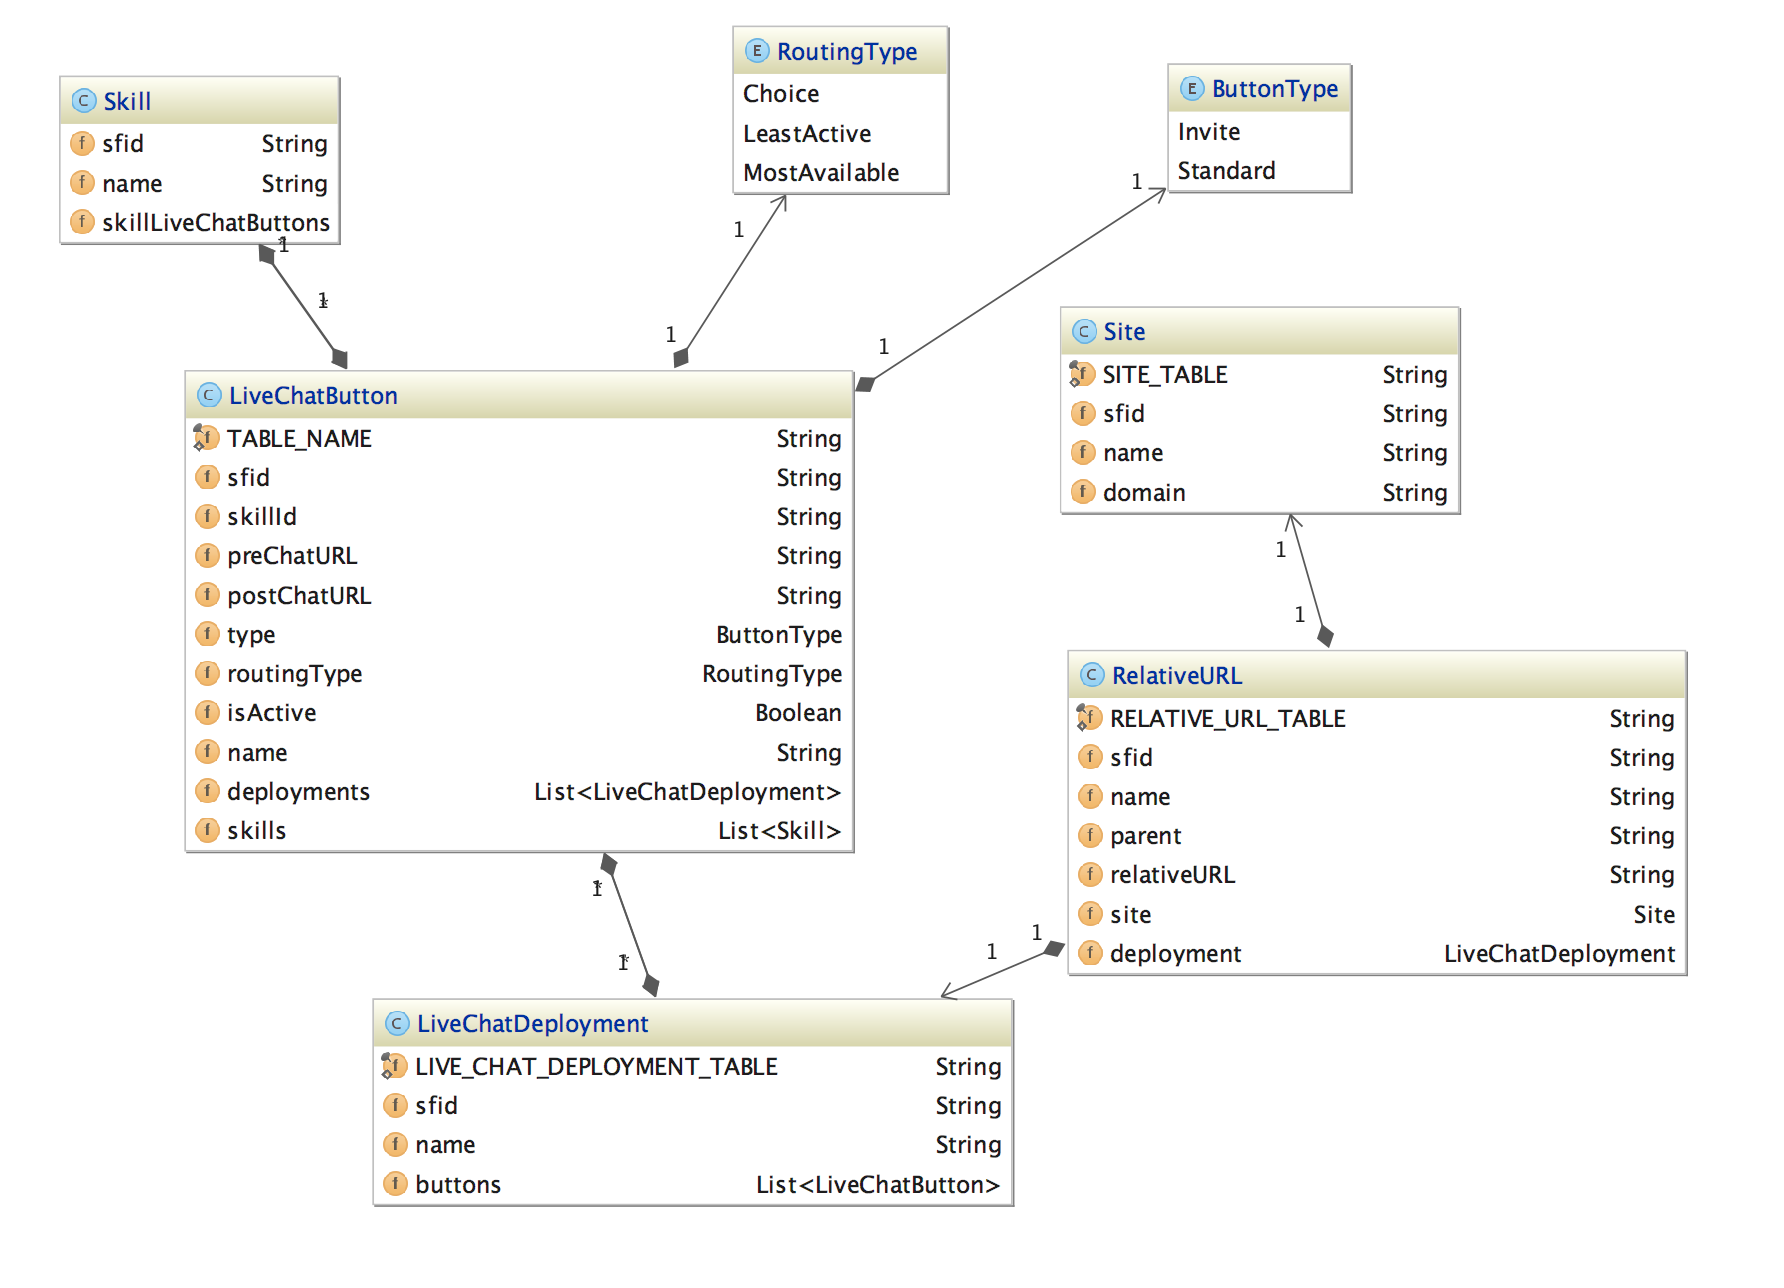
\includegraphics[scale=0.4]{sf-domain.png}  
  \caption{Диаграмма классов интеграции с Salesforce}
  \label{fig:sf-domain}
\end{figure} 

Для интеграции с  сервисом, клиент должен разместить сниппет, который он может найти в Salesforce CRM. После того как сниппет подгрузится на странице пользователя, он делает запрос на извлечение данных необходимых для подгрузки онлайн чата. После того как сниппет был отправлен и аутентифицирован, запрос перенаправляется в salesforce-integration microservice. 

В нем определяется, с какой страницы был произведен запрос, и дальше ищется в базе синтегрированной с  SF, к какой связке (Site, RelativeURL) она больше всего подходит. Дальше из этой связки достаются нужные объекты OrganizationID, DeploymentId, SkillID и Callback. Следующий шаг -- это найти все подходящие LiveChatButton. Они определяются по найденным объектам DeploymentID и SkillID. После того, как вся нужная информация собрана (OrganizationID, DeploymentId, SkillID, Callback и список LiveChatButton) она передается в браузер клиенту, и в нём подгружается Salesforce онлайн-чат по пришедшим параметрам.

После того, как он подгрузился, выполняется дополнительный callback, переданный из SF, который позволяет выполнить любые дополнительные действия, нужные в тех или иных случаях. 

На рисунке~\ref{fig:chat-integration} приведена схема интеграции.
% \pagebreak
\begin{figure}[h]
\centering
  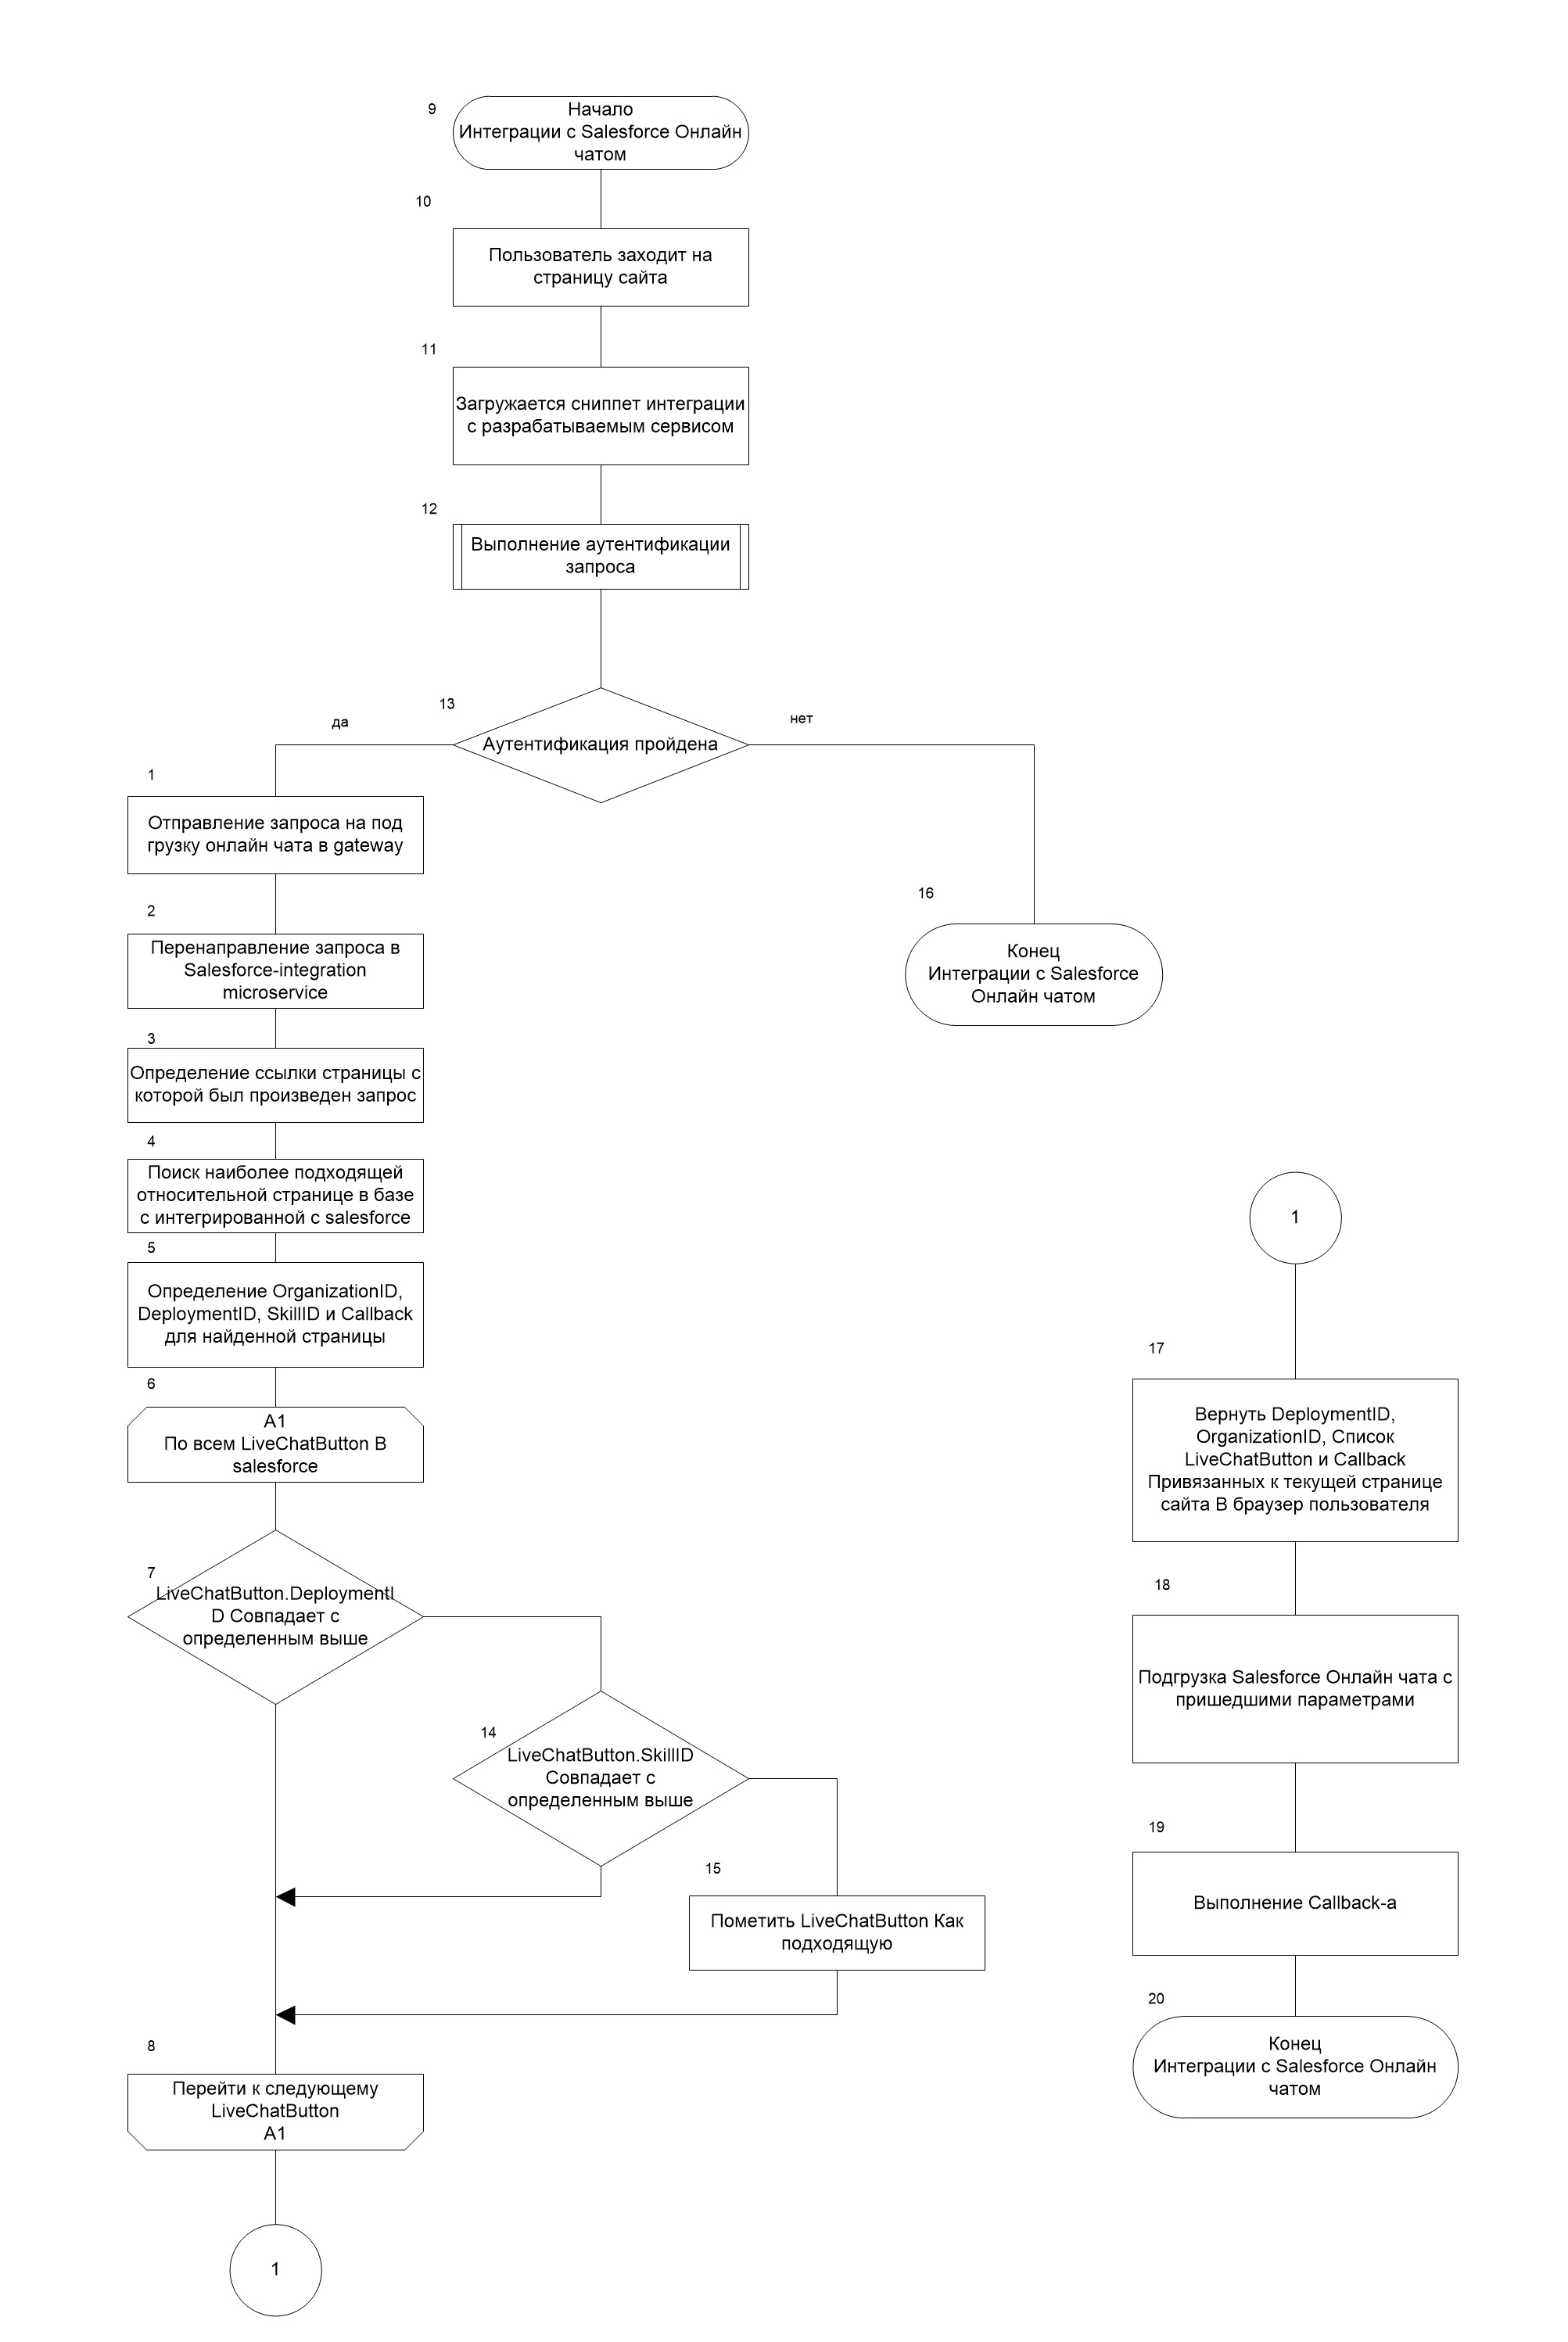
\includegraphics[scale=0.20]{sf-chat-integration.jpg}  
  \caption{Схема интеграции с Salesforce online chat}
  \label{fig:chat-integration}
\end{figure} 




% Глава ? Тестирование приложения
\section{Тестирование приложения}
\label{sec:testing}


\subsection{Тестирование панели администратора}
Для оценки правильности работы функциональных требований в панели администратора было проведено тестирование, включающие тест кейсы представленные      в таблице~\ref{table:testing:admin} 
  
\begin{longtable}[l]{| >{\raggedright}m{0.3\textwidth}
                  | >{\raggedright}m{0.4\textwidth}
                  | >{\raggedright\arraybackslash}m{0.2\textwidth}|}
  \caption{Тестирование микросервиса панели администратора}
  \label{table:testing:admin} \tabularnewline


    \hline
    Название тест-кейса и его описание & Ожидаемый результат  & Полученный результат \\
    \hline
    \centering{1} & \centering{2} & \centering{3} \tabularnewline
    \hline

    Авторизация в панель администратора \\
    a) Зайти на страницу входа в аккаунт панель администратора \\
    б) Ввести логин и пароль \\
    в) Нажать кнопку Login 

    & 

    a) Отображается страница входа в аккаунт панель администратора \\
    б) Необходимые поля доступны для заполнения \\
    в) Вход в панель администратора

    & 

    Пройден \\ \hline

    % Создание нового события
    Создание нового события \\
    a) Перейти на страницу создания нового события \\
    б) Ввести обязательные поля \\
    в) Нажать кнопку Create 

    & 

    a) Отображается страница создания нового события \\
    б) Необходимые поля доступны для заполнения \\
    в) Событие успешно создано 
    
    & 

    Пройден \\ 

    \pagebreak
    \caption*{Продолжение таблицы~\ref{table:testing:admin}} \\
    \hline
    \centering 1 & \centering 2 & \centering 3 \tabularnewline
    \hline


    % Добавление поля для события
    Добавление поля для события\\
    a) Выбрать события \\
    б) Нажать кнопку Add Prop \\
    в) Ввести обязательные поля \\
    г) Нажать кнопку Add 

    & 

    a) Отображается страница события \\
    б) Отображается popup добавления поля события \\
    в) Необходимые поля доступны для заполнения \\
    г) Поле успешно добавлено в событие 
    
    & 

    Пройден \\ \hline

    Просмотр онлайн статистики поступление событий \\
    а) Зайти в панель администратора \\
    б) Перейти на страницу статистики 
    
    & 

    а) Отображается главной страницы  \\
    б) Отображается график текущих поступающими событиями, который изменять с течение времени без перезагрузки страницы 
    
    & 

    Пройден \\

    % \pagebreak
    % \caption*{Продолжение таблицы~\ref{table:testing:admin}} \\
    % \hline
    % \centering 1 & \centering 2 & \centering 3 \tabularnewline
    \hline


    % Просмотр статисти поступивших событий за промежуток времени
    Просмотр статистики поступивших событий за промежуток времени \\
    a) Зайти в панель администратора \\
    б) Перейти на страницу статистики \\
    в) Выбрать интервал времени \\
    г) Нажать кнопку Show 
    
    & 

    a) Отображается главной страницы  \\
    б) Отображается график текущих поступающими событиями, который изменять с течение времени без перезагрузки страницы \\
    в) Необходимые поля доступны для заполнения \\
    г) Отображается график поступивших событий за выбранный промежуток 
    
    & 

    Пройден \\ \hline

  \hline

\end{longtable}


Таким образом результат тестирования подтверждает, что микросервис ответственный за панель администратора работает корректно с установленными требованиями.

\subsection{Тестирование интеграции с Salesforce CRM}
Для оценки правильности работы функциональных требований связанных с интеграцией salesforce было проведено тестирование, включающие тест кейсы представленные в таблице~\ref{table:testing:sf} 


\begin{longtable}[l]{| >{\raggedright}m{0.3\textwidth}
                  | >{\raggedright}m{0.3\textwidth}
                  | >{\raggedright\arraybackslash}m{0.3\textwidth}|}
  \caption{Тестирование микросервиса интеграции с Salesforce CRM}
  \label{table:testing:sf} \tabularnewline

  \hline
       Название тест-кейса и его описание & Ожидаемый результат  & Полученный результат \\
    \hline
    \centering{1} & \centering{2} & \centering{3} \tabularnewline
    \hline

   % Тестирование онлайн чата
    Тестирование настроек онлайн чата в sf \\
    a) Агент заходит в Salesforce CRM \\
    б) Агент настраивает параметры в salesforce для онлайн чата (специфика sf) \\
    в) Агент настраивает страницу сайта клиента, на которой должен появляться чат с пользователем \\
    г) Агент заходить Salesforce Console
    & 
    a) Отображается главной страница Salesforce CRM \\
    б) Параметры доступны для настройки \\
    в) Необходимые поля доступны для заполнения \\
    г) Отображается Salesforce Console доступна
    & 
    Пройден \\ 

    \pagebreak
    \caption*{Продолжение таблицы~\ref{table:testing:admin}} \\
    \hline
    \centering 1 & \centering 2 & \centering 3 \tabularnewline
   
    \hline

    Тестирование онлайн чата \\
    a) Агент ставит в Salesforce Console себе статус онлайн \\
    б) Пользователь заходит на страницу сайта, на которой настроен онлайн чат \\
    в) Выполняются условия по котором должен показаться онлайн чат \\
    г) Пользователь нажимает кнопку Start Chat \\
    д) Агент нажимает кнопку принять чат \\
    е) Агент отправляет сообщение \\
    ж) Пользователь отправляет сообщение \\
    з) Пользователь закрывает чат 
    
    & 

    a) Агенту проставляется статус онлайн \\
    б) Страница сайта корректно загружается \\
    в) На странице всплывает окошко для онлайн чата \\
    г) Открывается окно ожидание онлайн чата с агентом и у агента в Salesforce Console отображается входящий вызов  \\
    д) Открывается чат с агентом \\
    е) Пользователь видит сообщение \\
    ж) Агент видит сообщение \\
    з) Чат успешно закрывается 
    
    & 
    
    Пройден \\ \hline

\end{longtable}
  
Таким образом результат тестирования подтверждает, что микросервис ответственный за интеграцию с salesforce работает корректно с установленными требованиями.

\subsection{Тестирование отказоустойчивости}
Для оценки работы системы в непредвиденных ситуациях (например проблемы с сетью, проблемы у интернет провайдера или вообще сгорел сервер) было проведено тестирование отказоустойчивости системы, включающие тест кейсы представленные в таблице~\ref{table:testing:fb} 
\begin{longtable}[l]{| >{\raggedright}m{0.3\textwidth}
                  | >{\raggedright}m{0.3\textwidth}
                  | >{\raggedright\arraybackslash}m{0.3\textwidth}|}
  \caption{Тестирование отказоустойчивости системы}
  \label{table:testing:fb} \tabularnewline

  \hline
       Название тест-кейса и его описание & Ожидаемый результат  & Полученный результат \\
    \hline
    \centering{1} & \centering{2} & \centering{3} \tabularnewline
    \hline


    Тестирование отказоустойчивости падения одного процесса микросервиса \\
    а) Запустить 2 экземпляра микросервиса ответственного за интеграцию с salesforce
    б) Администратор заходит в Hystrix Dashboard \\
    в) Администратор вводит соответствующую ссылку /turbine/turbine.stream в поле для заполнение и нажимает кнопку Monitor Stream \\
    г) С эмулировать падение процесса сервиса: на сервере убить процесс микросервиса ответственного за интеграцию с salesforce с помощью команды kill -9 PID (PID - id процесса) \\
    & 
    Тестирование отказоустойчивости падения одного процесса микросервиса \\
    а) Поднялась 2 процесса микросервиса ответственного за интеграцию с salesforce \\
    б) Отображается главная страница Hystrix Dashboard \\
    в) Отображается dashboard с real-time графиками состояний статусов происходящих событий в системе \\
    г) Система по-прежнему работает \\
    & 
    Пройден \\ 

    \pagebreak
    \caption*{Продолжение таблицы~\ref{table:testing:fb}} \\
    \hline
    \centering 1 & \centering 2 & \centering 3 \tabularnewline
   
    \hline


    % Тестирование отказоустойчивости
    Тестирование отказоустойчивости падения всех процессов микросервиса \\
    a) Администратор заходит в Hystrix Dashboard \\
    б) Администратор вводит соответствующую ссылку /turbine/turbine.stream в поле для заполнения и нажимает кнопку Monitor Stream \\
    в) С эмулировать падение сервиса: на сервере последовательно аварийно завершить все процессы микросервиса, ответственного за интеграцию с salesforce с помощью команды kill -9 PID (PID - id процесса) \\
    г) Запустить микросервис ответствененный за интеграцию с salesforce
    & 
    Тестирование отказоустойчивости падения всех процессов микросервиса \\
    a) Отображается главная страница Hystrix Dashboard \\
    б) Отображается dashboard с real-time графиками состояний статусов происходящих событий в системе \\
    в) На графики интеграции с salesforce разомкнулся Circle Breaker, вследствие чего график стал красным и запросы перестали отправляться в сервис интеграции. Вместо этого стали выполняться fallback методы \\
    г) Circle Breaker замкнулся, вследствие чего запросы опять стали ходить в микросервис интеграции с salesforce
    & 
    Пройден \\ \hline

\end{longtable}



% Глава ? Руководство пользователя
\section{Руководство пользователя}
\label{sec:manual:intro}

\subsection{Руководство по разворачиванию приложения}
\label{sub:manual:deploy}

Приложения разрабатывалось с помощью package manager-а gradle, в котором прописаны все необходимые сторонние библиотеки, таким образом все нужный зависимости для проекта скачаются автоматически. Зависимости для UI собирались с помощь package manager-а npm, поэтому они так же скачаются автоматически, при сборке проекта.

Приложение использует следующие базы данных и сервисы:
\begin{itemize}
\item postgreSQL 9.3;
\item mongoDB 3.0;
\item redis 3.2;
\item rabbitMQ 3.6;
\item salesforce;
\item fullContact.
\end{itemize}

Всю конфигурацию для подключения баз данных и внешних сервисов, нужно прописывать в соответствующих файлах в git репозитории конфигурации:
\begin{itemize}
\item конфигурацию для подключению баз данных PostgreSQL, MongoDB, Redis, RabbitMQ в файле ets-service.yml;
\item конфигурацию для подключению Salesforce и с интегррованой с ним базой в файле salesforce-integration.yml;
\item конфигурацию для подключения сервиса предоставления публичной информации FullContact в файле social-integration.yml;
\item после того как соответствующая конфигурция будет прописана, нужно выполнить стандартные комманды git-а: git commit -а и git push.
\end{itemize}

После этого, чтобы собрать приложение нужно выполнить команду gradle build.

Если нужно запустить отдельный микросервис то его можно запустить соответствующей командой gradle :{microservice-name}:bootRun, где {microservice-name} имя микросервиса.

Для простоты разворачивания всех микросервисов сразу, был написан docker-compose.yml файл, с помощью которого одной командой docker-compose up, можно запустить все микросервисы сразу в docker контейнерах. Кроме того, он дает возможность легко горизонтально масштабировать отдельные микросервисы. 

Например: командой  docker-compose scale ets-service=5, поднимется 5 экземпляров микросервиса ets-service, и с помощью Ribbon другие микросервисы будут балансировать нагрузку по ним при обращении к сервису ets-service.

Для просмотра информации о развернутых серверов и их состояниях, можно зайти на {host:8761}, где host -- это адрес где развернут микросервис discovery-client (рисунок~\ref{fig:dc}).

\begin{figure}[h]
\centering
  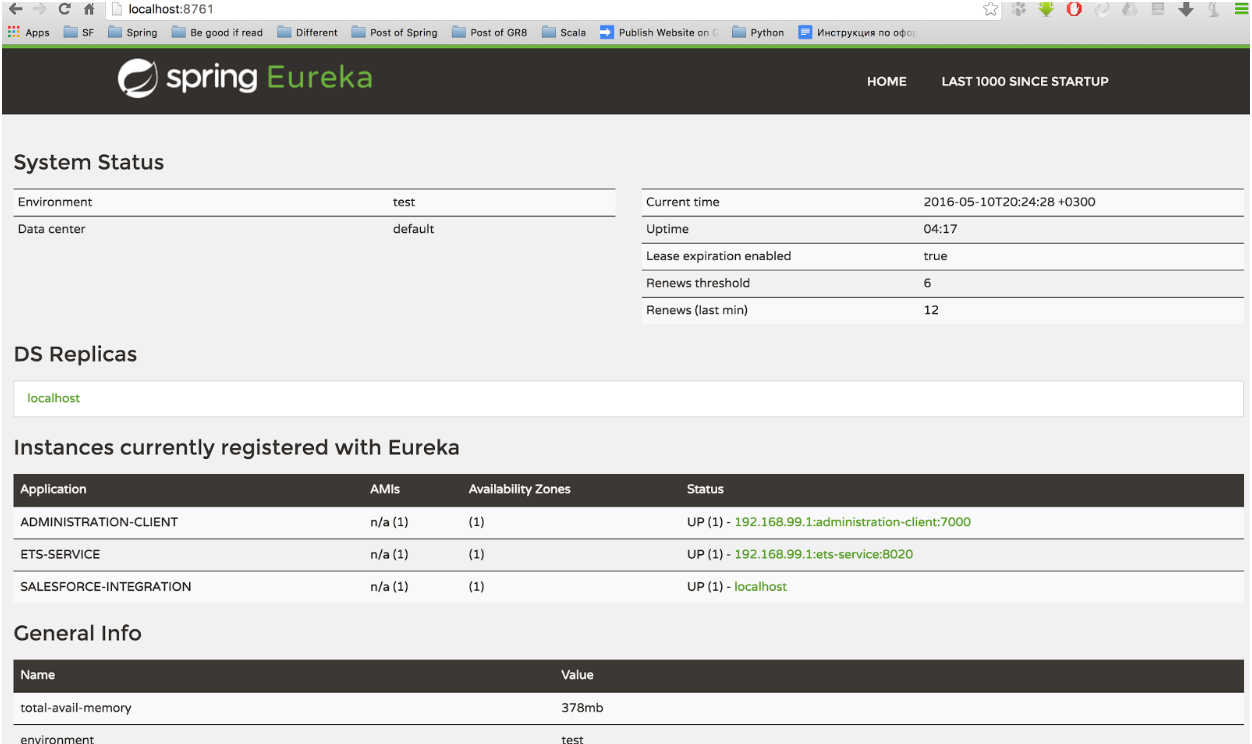
\includegraphics[scale=0.6]{dc.png}  
  \caption{Discovery client interface}
	\label{fig:dc}
\end{figure} 


\subsection{Руковоство для администраторов}
\label{sub:manual:admin}

В рамках данного проекта была также разработана панель администратора, в которой администраторы и менеджеры могут создавать/удалять/изменять и настраивать модели событий, которые будет поддерживать система, а так же возможность просмотра реал-тайм статистики происходящих событий. В рамках данной работы, постройка сложного UI не предполагалась, а наоборот цель была построить как можно более минималистический интерфейс, для проверки концепции архитектуры данной системы. 

На рисунке ~\ref{fig:events}, можно увидеть интерфейс на котором можно настраивать модели события под свои нужды.

\pagebreak
\begin{figure}[h]
\centering
  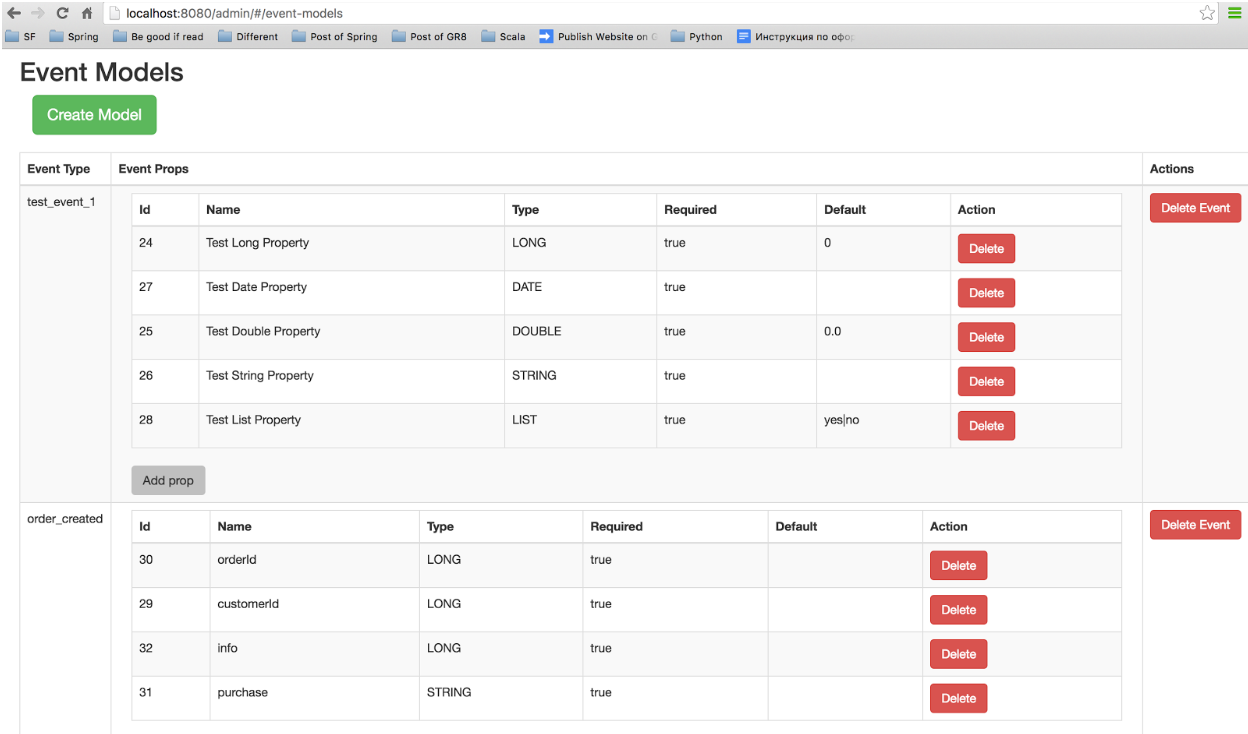
\includegraphics[scale=0.6]{events.png}  
  \caption{Интерфейс настройки моделей событий}
	\label{fig:events}
\end{figure}

На рисунке ~\ref{fig:event-prop} показано как выглядит интерфейс добавления и изменения того или иного поля в модели события.

\begin{figure}[h]
\centering
  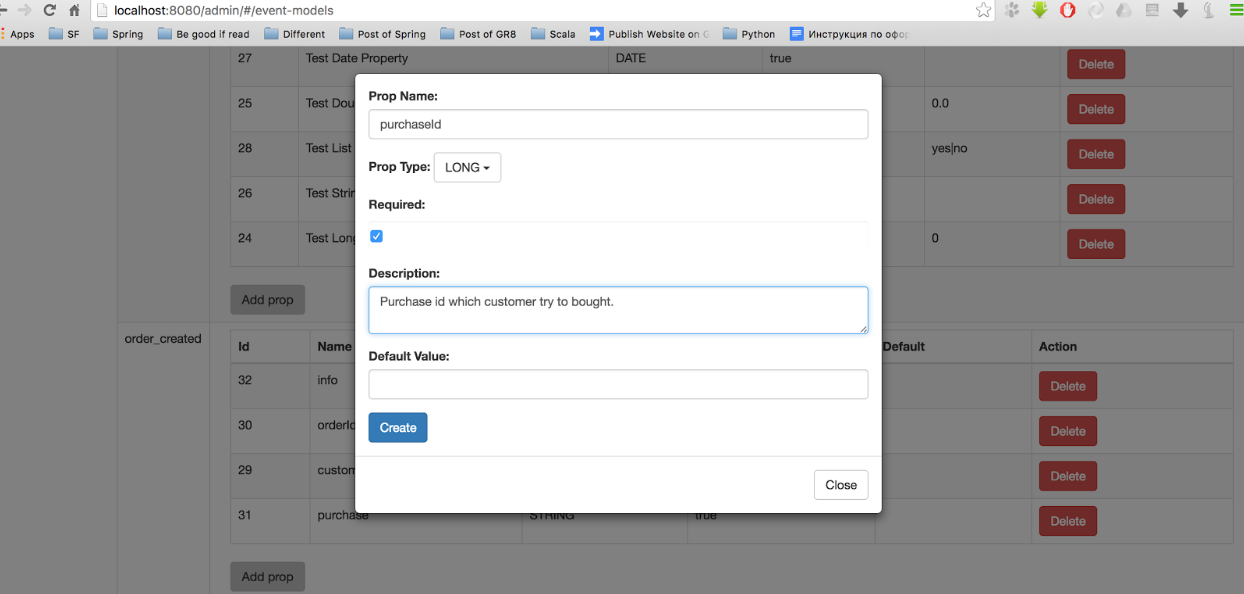
\includegraphics[scale=0.6]{event-prop.png}  
  \caption{Интерфейс настройки поля модели события}
	\label{fig:event-prop}
\end{figure}

Интерфейс просмотра статистики изображен на рисунке ~\ref{fig:stats}.
Так же на нем существует возможность просмотра статистики за определенный период. Для этого нужно всего ли выбрать соответствующий период.


\pagebreak
\begin{figure}[ht]
\centering
  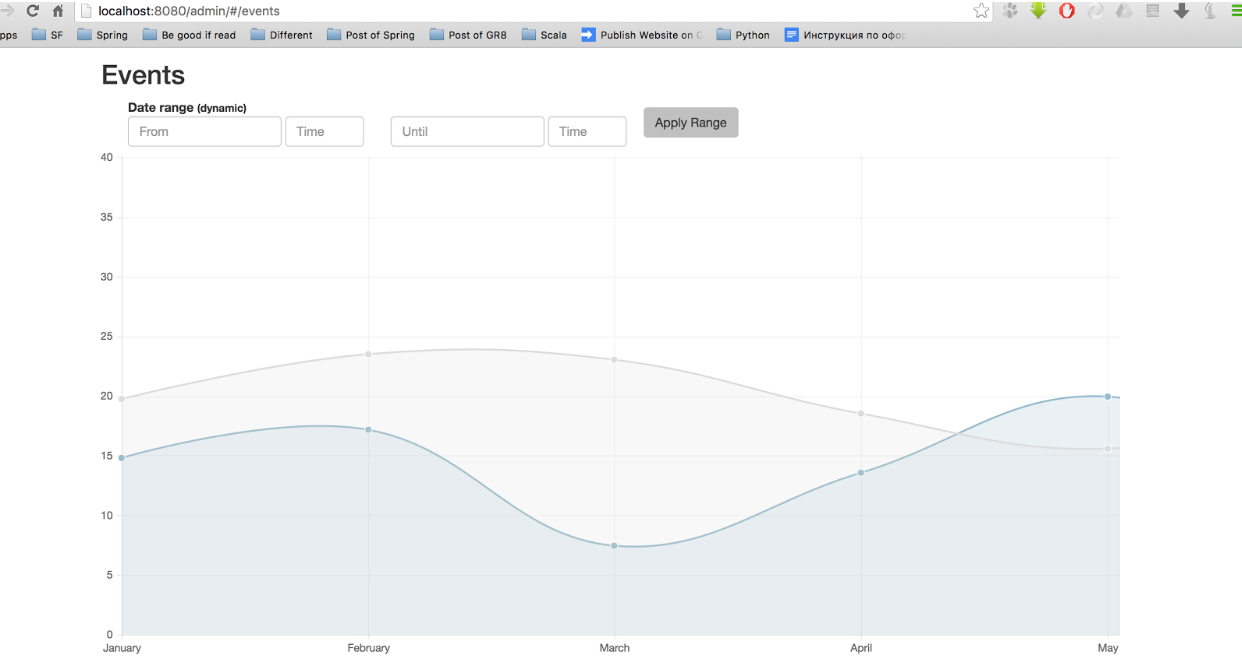
\includegraphics[scale=0.8]{stats.png}  
  \caption{Интерфейс просмотра статистики}
	\label{fig:stats}
\end{figure}

Наблюдать за состояниями микросервисов администраторы могут с помощью Hystrix Dashboard. Чтобы в него зайти нужно открыть страницу /hystrix-dashboard на которой будет поле для ввода источника данных для hystrix (https://hostname:port/turbine/turbine.stream).

На рисунке~\ref{fig:hystrix-m} изображен Hystrix Dashboard разрабатываемого программного средства.
\pagebreak
\begin{figure}[h]
\centering
  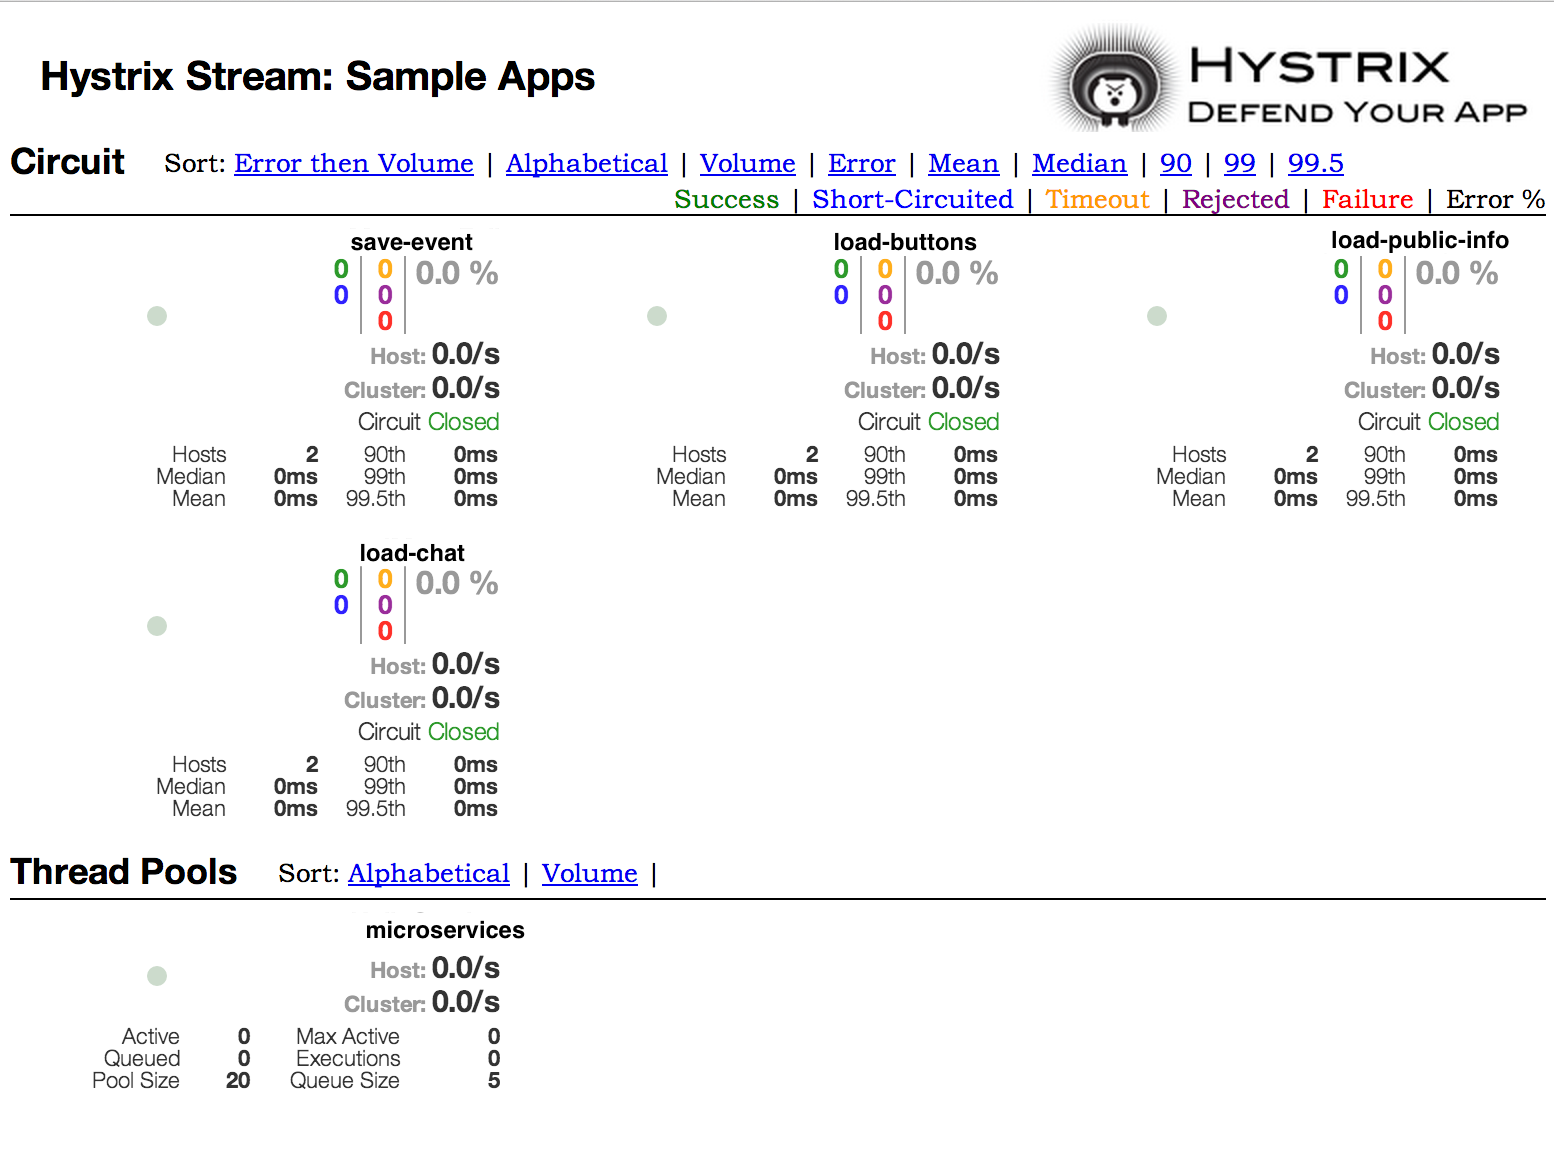
\includegraphics[scale=0.2]{hystrix.png}  
  \caption{Hystrix Dashboard программного средства}
  \label{fig:hystrix-m}
\end{figure} 



\subsection{Руководство по интеграции с онлайн чатом}
\label{sub:manual:chat}
На стороне salesforce есть множество настроек и критериев, по которым можно настроить онлайн чат под свои нужды. И в данный проект не подразумевает описание того как работает Salesforce. Подразумевается, что агенты которые будут общаться с посетителями через онлайн чат Salesforce, знаю его и умеют с ним работать. 
Со стороны агента чат будет как на рисунке ~\ref{fig:sf-chat}, также там предоставляются объекты Contact и Case в которых он заполняет, всё необходимую информацию собранную у клиента.

\begin{figure}[ht]
\centering
  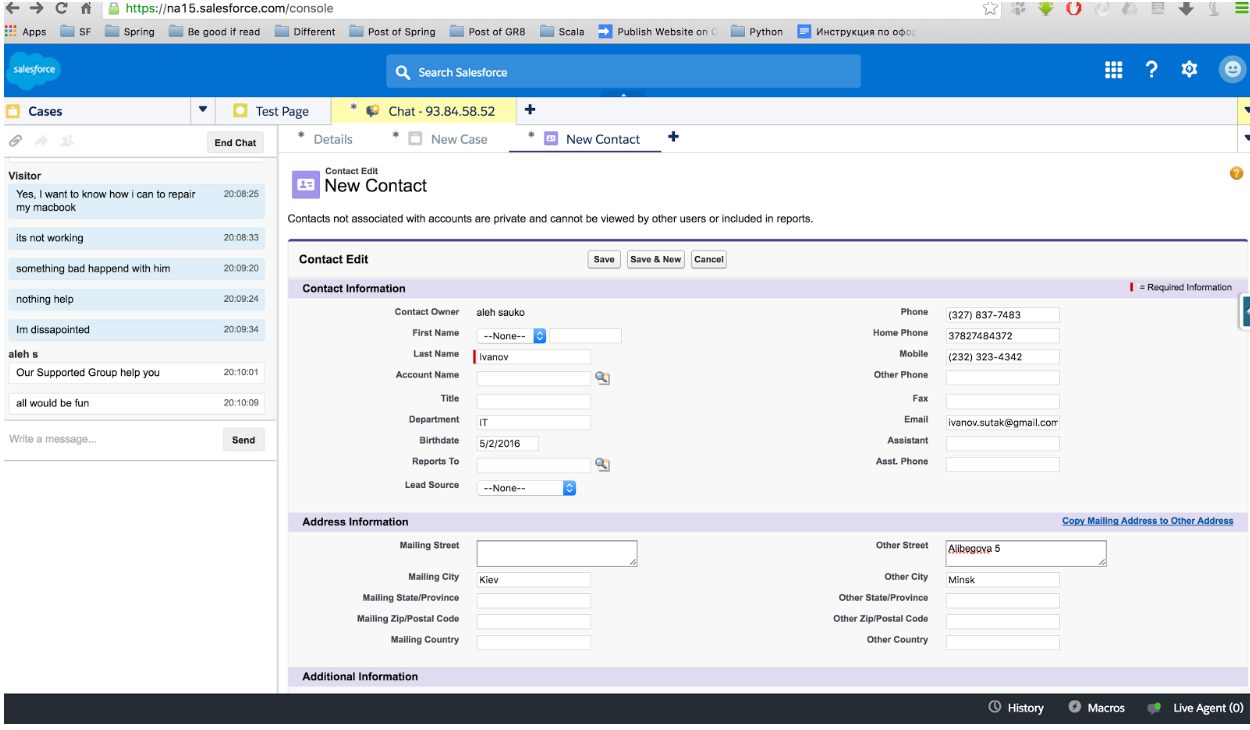
\includegraphics[scale=0.6]{sf-chat.png}  
  \caption{Salesforce online chat}
  \label{fig:sf-chat}
\end{figure}



\pagebreak
На стороне посетителя, чат выглядит как на рисунке ~\ref{fig:cl-chat}.

\begin{figure}[ht]
\centering
  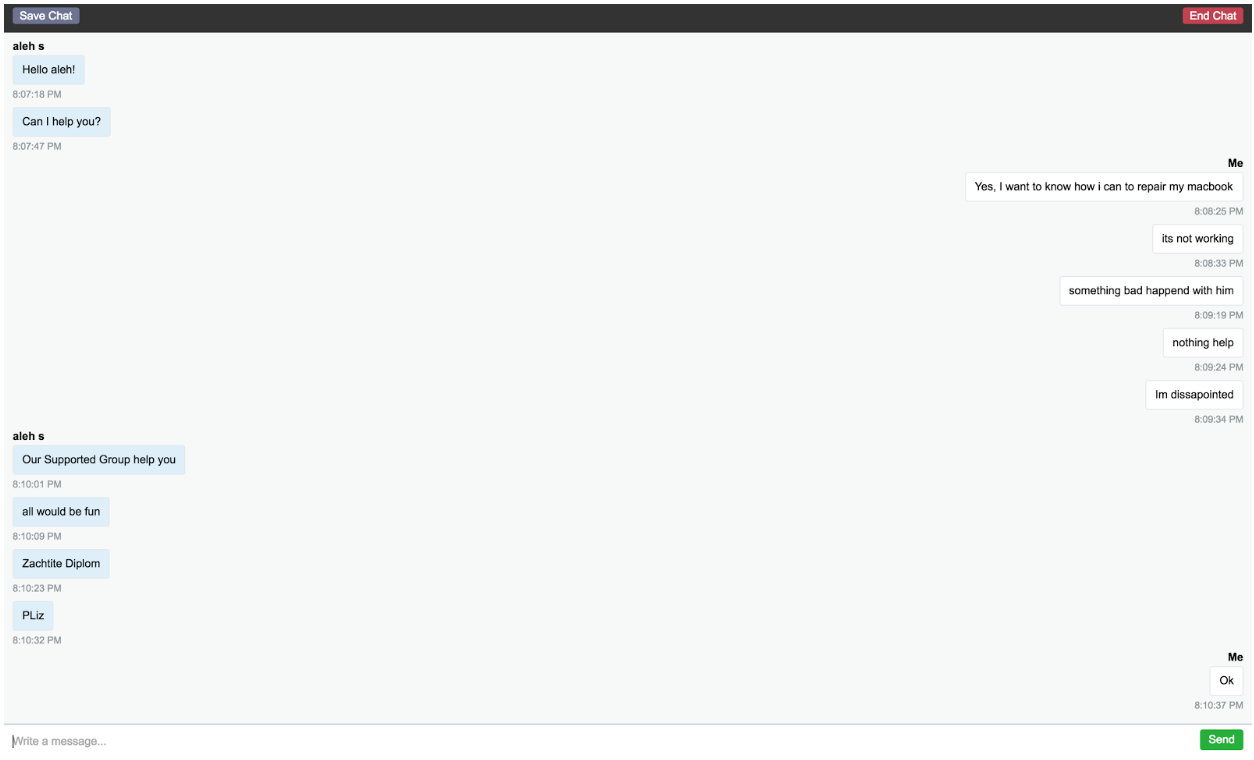
\includegraphics[scale=0.6]{cl-chat.png}  
  \caption{Client side chat}
  \label{fig:cl-chat}
\end{figure}

% Глава ? Технико-экономическое обоснование
\def \byr{Br}

\section{Технико-экономическое обоснование разработки ПС}

% Категория сложности
\def \complexityGroup{3}

% Категория новизны
\def \noveltyGroup{Б}

% ---

Целью дипломного проектирования является создание информационно-аналитического программного средства для взаимодействия клиента с сайтом с целью увеличения продуктивности последнего. Данное ПС реализует интеграцию сайта с различными CRM-системами, создания профиля пользователя, а также собирание статистики и действий произведенных им на сайте. Основными достоинствами программного средства являются: cистема отслеживания событий приспособленная для интеграции с такими внешними сервисами, как ContactInfo, Salesforce CRM; микросервисная архитектура, позволяющая горизонтально масштабировать отдельные сервисы и легко добавлять новые интеграции с внешними источниками.

В данном разделе рассмотрим экономическую эффективность программного средства. Для оценки экономической эффективности разработанного программного средства необходимо рассчитать смету затрат на разработку, цену и прибыль продажи одной программной системы.

Программный комплекс относится к \complexityGroup-й группе сложности. Категория новизны продукта – <<\noveltyGroup>>.

Расчеты выполнены на основе методического пособия ~\cite{palicyn_2006}.



\subsection{Расчёт сметы затрат и цены программного продукта}

% Коэффициент сложности, ед.
\def \additionalComplexityFactor{0.12}
\FPeval{complexityFactor}{clip(1 + \additionalComplexityFactor)}

% Степень использования при разработке стандартных модулей, ед.
\def \stdModuleUsageFactor{0.6}

% Коэффициент новизны, Кн
\def \noveltyFactor{0.9}

% Годовой эффективный фонд времени, дн.
\def \daysInYear{366}
\def \holidaysInYear{6}
\def \weekendDaysInYear{105}
\def \vacationDaysInYear{24}
\FPeval{workingDaysInYear}{
    clip(\daysInYear -
         \holidaysInYear -
         \weekendDaysInYear -
         \vacationDaysInYear)
}

% Среднемесячная норма рабочего времени, Фр
\def \workingHoursInMonth{160}

% Продолжительность рабочего дня, ч.
\def \workingHoursInDay{8}

% Месячная тарифная ставка первого разряда, Br
% \def \tariffRate{298000} % Гос. предприятия
\def \tariffRate{450000}

% Коэффициент премирования, ед
\def \bonusRate{1.5}

% Норматив дополнительной заработной платы, Br
\def \additionalSalaryRate{20}

% Норматив отчислений в ФСЗН и обязательное страхование, %
\def \socialProtectionRate{34}

% Норматив отчислений в Белгосстрах
\def \bgsRate{0.7}

% Норматив командировочных расходов, %
\def \businessTripRate{15}

% Норматив прочих затрат, %
\def \otherExpenseRate{20}

% Норматив накладных расходов, %
\def \overheadExpenseRate{100}

% Прогнозируемый уровень рентабельности, %
\def \profitability{35}

% Норматив отчислений в местный и республиканский ю.джет
\def \localRepubTaxRate{3.9}

% Норматив НДС, %
\def \vatRate{20}

% Норматив налога на прибыль, %
\def \profitTaxRate{18}

% Норматив расхода материалов, %
\def \materialsRate{3}

% Норматив расхода машинного времени, ч.
\def \debugRate{15} % часов / 100 строк кода

% Цена одного часа машинного времени, Br
\def \machineHourCost{25000}

% Норматив расходов на сопровождение и адаптацию ПО, %
\def \supportAndAdaptationRate{30}

% ---

Исходные данные для разрабатываемого проекта указаны в таблице~\ref{table:economics:initial_data}.

На основании сметы затрат и анализа рынка ПО определяется плановая отпускаемая цена.
Для составления сметы затрат на создание ПО необходима предварительная оценка трудоемкости ПО и его объёма.
Расчет объёма программного продукта (количества строк исходного кода) предполагает определение типа программного обеспечения, всестороннее техническое обоснование функций ПО и определение объёма каждой функций.
Согласно классификации типов программного обеспечения~\cite[с.~59,~приложение 1]{palicyn_2006}, разрабатываемое ПО с наименьшей ошибкой можно классифицировать как ПО методo"=ориентированных расчетов.
\pagebreak

\begin{longtable}{| >{\raggedright}m{0.62\textwidth}
                  | >{\centering}m{0.17\textwidth}
                  | >{\centering\arraybackslash}m{0.13\textwidth}|}
    \caption{Исходные данные}
    \label{table:economics:initial_data}
    \\

    \hline
    {\begin{center} Наименование \end{center} } & Условное обозначение & Значение
    \\ \hline

    Категория сложности
    & & \complexityGroup
    \\ \hline

    Коэффициент сложности, ед.
    & $ \text{К}_\text{с} $ & \num{\complexityFactor}
    \\ \hline

    Степень использования при разработке стандартных модулей, ед.
    & $ \text{К}_\text{т} $ & \num{\stdModuleUsageFactor}
    \\ \hline

    Коэффициент новизны, ед.
    & $ \text{К}_\text{н} $ & \num{\noveltyFactor}
    \\ \hline

    Годовой эффективный фонд времени, дн.
    & $ \text{Ф}_\text{эф} $ & \num{\workingDaysInYear}
    \\ \hline

    Продолжительность рабочего дня, ч.
    & $ \text{Т}_\text{ч} $ & \num{\workingHoursInDay}
    \\ \hline

    Месячная тарифная ставка первого разряда, \byr{}
    & $ \text{Т}_{\text{м}_{1}}$ & \num{\tariffRate}
    \\ \hline

    Коэффициент премирования, ед.
    & $ \text{К} $ & \num{\bonusRate}
    \\ \hline

    Норматив дополнительной заработной платы, ед.
    & $ \text{Н}_\text{д} $ & \num{\additionalSalaryRate}
    \\ \hline

    Норматив отчислений в ФСЗН, $\%$
    & $ \text{Н}_\text{сз} $ & \num{\socialProtectionRate}
    \\ \hline

    Норматив отчислений в Белгосстрах, $\%$
    & $ \text{Н}_\text{с} $ & \num{\socialProtectionRate}
    \\ \hline

    Норматив командировочных расходов, $\%$
    & $ \text{Н}_\text{к} $ & \num{\businessTripRate}
    \\ \hline

    Норматив прочих затрат, $\%$
    & $ \text{Н}_\text{пз} $ & \num{\otherExpenseRate}
    \\ \hline

    Норматив накладных расходов, $\%$
    & $ \text{Н}_\text{рн} $ & \num{\overheadExpenseRate}
    \\ \hline

    Прогнозируемый уровень рентабельности,
    $\%$ & $ \text{У}_\text{рп} $ & \num{\profitability}
    \\ \hline

    Норматив НДС, $\%$
    & $ \text{Н}_\text{дс} $ & \num{\vatRate}
    \\ \hline

    Норматив налога на прибыль, $\%$
    & $ \text{Н}_\text{п} $ & \num{\profitTaxRate}
    \\ \hline

    Норматив расхода материалов, $\%$
    & $ \text{Н}_\text{мз} $ & \num{\materialsRate}
    \\ \hline

    Норматив расхода машинного времени, ч.
    & $ \text{Н}_\text{мв} $ & \num{\debugRate}
    \\ \hline

    Цена одного часа машинного времени, \byr{}
    & $ \text{Н}_\text{мв} $ & \num{\machineHourCost}
    \\ \hline

    Норматив расходов на сопровождение и адаптацию ПО, $\%$
    & $ \text{Н}_\text{рса} $ & \num{\supportAndAdaptationRate}
    \\ \hline
\end{longtable}


Общий объём программного продукта определяется исходя из количества и объёма функций, реализованных в программе:
\begin{equation}
  \label{eq:economics:total_loc}
  V_{o} = \sum_{i = 1}^{n} V_{i} \text{\,,}
\end{equation}
\begin{explanation}
где & $ V_{i} $ & объём отдельной функции ПО, LoC; \\
    & $ n $ & общее число функций.
\end{explanation}

На стадии технико-экономического обоснования проекта рассчитать точный объём функций невозможно.
Вместо вычисления точного объёма функций применяются приблизительные оценки на основе данных по аналогичным проектам или по нормативам~\cite[с.~61,~приложение 2]{palicyn_2006}, которые приняты в организации.

\def \totalLOC{9710} % TODO
\def \totalLOCCorrected{6390} % TODO

\begin{longtable}{| >{\centering}m{0.12\textwidth}
                  | >{\raggedright}m{0.40\textwidth}
                  | >{\centering}m{0.18\textwidth}
                  | >{\centering\arraybackslash}m{0.18\textwidth}|}
  \caption{Перечень и объём функций программного модуля}
  \label{table:econ:function_sizes}
  \\

  \hline
    \multirow{2}{0.12\textwidth}[-0.5em]{\centering \No{} функции}
    & \multirow{2}{0.40\textwidth}[-0.55em]{\centering Наименование (содержание)}
    & \multicolumn{2}{c|}{\centering Объём функции, LoC} \tabularnewline

  \cline{3-4} &
       & { по каталогу ($ V_{i} $) }
       & { уточненный ($ V_{i}^{\text{у}} $) } \tabularnewline
  \hline

  101 & Организация ввода информации
  & \num{620} & \num{450}
  \\ \hline

  405 & Система настройки ПО
  & \num{1650} & \num{1500}
  \\ \hline

  502 & Монитор система (управление работой комплекса ПО)
  & \num{1100} & \num{900}
  \\ \hline

  301 & Интерфейс к базе данных моделей и данных аутентификации
  & \num{790} & \num{650}
  \\ \hline

  305 & Защита от несанкционированного доступа к базе
  & \num{820} & \num{400}
  \\ \hline

  501 & Монитор ПО (управление работой компонентов)
  & \num{1240} & \num{1010}
  \\ \hline

  506 & Обработка исключительных ситуаций
  & \num{620} & \num{400}
  \\ \hline

  507 & Обеспечение интерфейса между компонентами
  & \num{970} & \num{680}
  \\ \hline

  612 & Аутентификация на основе сравнения реальных данных и математической модели
  & \num{1100} & \num{800}
  \\ \hline

  Итог & &
  {\num{\totalLOC}} & {\num{\totalLOCCorrected}}
  \\ \hline

\end{longtable}

Перечень и объём функций программного модуля перечислен в таблице~\ref{table:econ:function_sizes}.
По приведенным данным уточненный объём некоторых функций изменился, и общий уточненный объём ПО
$ V_{\text{у}} = \SI{\totalLOCCorrected}{\text{LoC}} $
.



\subsection{Расчёт трудоемкости}

% Нормативная трудоёмкость, Тн
\def \normativeWorkload{144}

% Общая трудоёмкость, То
\FPeval{totalWorkload}{
    trunc(\normativeWorkload *
          \complexityFactor *
          \stdModuleUsageFactor *
          \noveltyFactor + 0.5, 0)
}

% Срок разработки проекта, Тр
\def \developmentMonths{3}
\FPeval{developmentYears}{round(\developmentMonths / 12, 2)}

% Численность исполнителей, Чр
\FPeval{requiredProgrammers}{trunc(\totalWorkload / (\developmentYears * \workingDaysInYear) + 0.5, 0) }

% Считаем, что работы каждому достаётся поровну.
\FPeval{workloadSenior}{trunc( \totalWorkload / \requiredProgrammers, 0 )}
\FPeval{workloadLead}{clip(\totalWorkload - \workloadSenior)}

% ---

На основании общего объема ПО определяется нормативная трудоемкость (
$ \text{Т}_\text{н}$
) с учетом сложности ПО. Для ПО \complexityGroup-ой группы сложности, к которой относится разрабатываемый программный продукт, нормативная трудоемкость составит~
$ \text{Т}_\text{н} = \SI{\normativeWorkload}{\text{чел.} / \text{дн.}} $

Нормативная трудоемкость служит основой для оценки общей трудоемкости~
$ \text{Т}_\text{о} $
.
Используем формулу (\ref{eq:economics:total_workload}) для оценки общей трудоемкости для небольших проектов:
\begin{equation}
  \label{eq:economics:total_workload}
  \text{Т}_\text{о} = \text{Т}_\text{н} \cdot
                      \text{К}_\text{с} \cdot
                      \text{К}_\text{т} \cdot
                      \text{К}_\text{н} \text{\,,}
\end{equation}
\begin{explanation}
где & $ \text{К}_\text{с} $ & коэффициент, учитывающий сложность ПО; \\
    & $ \text{К}_\text{т} $ & поправочный коэффициент, учитывающий степень использования при разработке стандартных модулей; \\
    & $ \text{К}_\text{н} $ & коэффициент, учитывающий степень новизны ПО.
\end{explanation}

Дополнительные затраты труда на разработку ПО учитываются через коэффициент сложности, который вычисляется по формуле
\begin{equation}
\label{eq:economics:additional_complexity_factor}
  \text{К}_{\text{с}} = 1 + \sum_{i = 1}^n \text{К}_{i} \text{\,,}
\end{equation}
\begin{explanation}
где & $ \text{К}_{i} $ & коэффициент, соответствующий степени повышения сложности ПО за счет конкретной характеристики; \\
    & $ n $ & количество учитываемых характеристик.
\end{explanation}

Наличие двух характеристик сложности позволяет~\cite[c.~66, приложение~4, таблица~П.4.2]{palicyn_2006} вычислить коэффициент сложности
\begin{equation}
\label{eq:economics:complexity_factor}
  \text{К}_{\text{с}} = \num{1} + \num{\additionalComplexityFactor} = \num{\complexityFactor} \text{\,.}
\end{equation}

Разрабатываемое ПО использует стандартные компоненты. Согласно справочным данным~\cite[c.~68,~приложение~4, таблица~П.4.5]{palicyn_2006} коэффициент использования стандартных модулей для разрабатываемого приложения
$ \text{К}_\text{т} = \num{\stdModuleUsageFactor} $
.

Согласно справочным данным~\cite[c.~67, приложение~4, таблица~П.4.4]{palicyn_2006}, коэффициент новизны для разрабатываемого ПО
$ \text{К}_\text{н} = \num{\noveltyFactor} $
.

Подставив приведенные выше коэффициенты для разрабатываемого ПО в формулу~(\ref{eq:economics:total_workload}) получим общую трудоемкость разработки
\begin{equation}
  \label{eq:economics:total_workload_calc}
  \text{Т}_\text{о} = \num{\normativeWorkload}
                      \cdot \num{\complexityFactor}
                      \cdot \num{\stdModuleUsageFactor}
                      \cdot \num{\noveltyFactor}
                    \approx \SI{\totalWorkload}{\text{чел.}/\text{дн.}}
\end{equation}

На основе общей трудоемкости и требуемых сроков реализации проекта вычисляется плановое количество исполнителей.
Численность исполнителей проекта рассчитывается по формуле:
\begin{equation}
  \label{eq:economics:num_of_programmers}
  \text{Ч}_\text{р} = \frac{\text{Т}_\text{о}}
                           {\text{Т}_\text{р}
                      \cdot \text{Ф}_\text{эф}} \text{\,,}
\end{equation}
\begin{explanation}
где & $ \text{Т}_\text{о} $ & общая трудоемкость разработки проекта, $ \text{чел.}/\text{дн.} $; \\
    & $ \text{Ф}_\text{эф} $ & эффективный фонд времени работы одного работника в течение года, дн.; \\
    & $ \text{Т}_\text{р} $ & срок разработки проекта, лет.
\end{explanation}

Эффективный фонд времени работы одного разработчика вычисляется по формуле
\begin{equation}
  \label{eq:economics:workload_per_programmer}
  \text{Ф}_\text{эф} = \text{Д}_\text{г} -
                       \text{Д}_\text{п} -
                       \text{Д}_\text{в} -
                       \text{Д}_\text{о} \text{\,,}
\end{equation}
\begin{explanation}
где & $ \text{Д}_\text{г} $ & количество дней в году, дн.; \\
    & $ \text{Д}_\text{п} $ & количество праздничных дней в году, не совпадающих с выходными днями, дн.; \\
    & $ \text{Д}_\text{в} $ & количество выходных дней в году, дн.; \\
    & $ \text{Д}_\text{п} $ & количество дней отпуска, дн.
\end{explanation}

Согласно данным, приведенным в производственном календаре для пятидневной рабочей недели в 2016 году для Беларуси~\cite{belcalendar_2016}, фонд рабочего времени составит
\begin{equation}
  \text{Ф}_\text{эф} = \num{\daysInYear} -
                       \num{\holidaysInYear} -
                       \num{\weekendDaysInYear} -
                       \num{\vacationDaysInYear}
                     = \SI{\workingDaysInYear}{\text{дн.}}
\end{equation}

Учитывая срок разработки проекта
$ \text{Т}_\text{р} = \SI{\developmentMonths}{\text{мес.}} = \SI{\developmentYears}{\text{года}} $
, общую трудоемкость и фонд эффективного времени одного работника, вычисленные ранее, можем рассчитать численность исполнителей проекта
\begin{equation}
  \label{eq:econ:num_of_programmers_calc}
  \text{Ч}_\text{р} = \frac{\num{\totalWorkload}}
                           {\num{\developmentYears}
                      \cdot \num{\workingDaysInYear}}
                    \approx \SI{\requiredProgrammers}{\text{рабочих}}.
\end{equation}

Вычисленные оценки показывают, что для выполнения запланированного проекта в указанные сроки необходимо \requiredProgrammers ~рабочих.



\subsection{Расчёт заработной платы исполнителей}

% Тариффные коэффициенты, Тк
\def \tariffFactorSenior{3.25} % == 14 разряд
\def \tariffFactorLead{3.48}   % == 15 разряд

% Часовая тарифная ставка исполнителей, Тч
\FPeval{hourlySalarySenior}{round( \tariffRate * \tariffFactorSenior / \workingHoursInMonth, 0 )}
\FPeval{hourlySalaryLead}{round( \tariffRate * \tariffFactorLead / \workingHoursInMonth, 0 )}

% Основная арплата, Зо
\FPeval{baseSalary}{
     round(\workingHoursInDay *
           \bonusRate *
           (\hourlySalarySenior * \workloadSenior +
            \hourlySalaryLead * \workloadLead), 0)
}

% Дополнительная зарплата, Зд
\FPeval{additionalSalary}{ round( \baseSalary * \additionalSalaryRate / 100, 0 ) }


% ---

Информация о работниках перечислена в таблице~\ref{table:economics:programmers}.
\begin{table}[ht]
  \caption{Работники, занятые в проекте}
  \label{table:economics:programmers}
  \begin{tabular}{| >{\centering}m{0.4\textwidth}
                  | >{\centering}m{0.15\textwidth}
                  | >{\centering}m{0.18\textwidth}
                  | >{\centering\arraybackslash}m{0.15\textwidth}|}
   \hline
   Исполнители & Разряд & Тарифный коэффициент & \mbox{Чел./дн.} занятости
   \\ \hline

   Программист \Rmnum{1}-категории & $ \num{14} $ & $ \num{\tariffFactorSenior} $ & $ \num{\workloadSenior} $
   \\ \hline
   Ведущий программист & $ \num{15} $ & $ \num{\tariffFactorLead} $ & $ \num{\workloadLead} $
   \\ \hline
  \end{tabular}
\end{table}

Месячная тарифная ставка одного работника вычисляется по формуле
\begin{equation}
  \label{eq:economics:monthly_salary}
  \text{Т}_\text{ч} =
    \frac {\text{Т}_{\text{м}_{1}} \cdot \text{Т}_{\text{к}} }
          {\text{Ф}_{\text{р}} }  \text{\,,}
\end{equation}
\begin{explanation}
где & $ \text{Т}_{\text{м}_{1}} $ & месячная тарифная ставка 1-го разряда, \byr; \\
    & $ \text{Т}_{\text{к}} $ & тарифный коэффициент, соответствующий установленному тарифному разряду; \\
    & $ \text{Ф}_{\text{р}} $ & среднемесячная норма рабочего времени, час.
\end{explanation}


Подставив данные из таблицы~\ref{table:economics:programmers} в формулу~(\ref{eq:economics:monthly_salary}), приняв значение тарифной ставки 1-го разряда
$ \text{Т}_{\text{м}_{1}} = \SI{\tariffRate}{\text{\byr}} $
и среднемесячную норму рабочего времени
$ \text{Ф}_{\text{р}} = \SI{\workingHoursInMonth}{\text{часов}} $
получаем
\begin{equation}
  \label{eq:economics:monthly_salary_senior}
  \text{Т}_{\text{ч}}^{\text{прогр. \Rmnum{1}-разр.}} =
      \frac{ \num{\tariffRate} \cdot \num{\tariffFactorSenior} }
           { \num{\workingHoursInMonth} }
    = \SI{\hourlySalarySenior}{\text{\byr}/\text{час;}}
\end{equation}
\begin{equation}
  \label{eq:economics:monthly_salary_lead}
  \text{Т}_{\text{ч}}^{\text{вед. прогр.}} =
      \frac{ \num{\tariffRate} \cdot \num{\tariffFactorLead} }
           { \num{\workingHoursInMonth} }
    = \SI{\hourlySalaryLead}{\text{\byr}/\text{час.}}
\end{equation}

Основная заработная плата исполнителей на конкретное ПО рассчитывается по формуле
\begin{equation}
  \label{eq:economics:base_salary}
  \text{З}_{\text{о}} = \sum^{n}_{i = 1}
                        \text{Т}_{\text{ч}}^{i} \cdot
                        \text{Т}_{\text{ч}} \cdot
                        \text{Ф}_{\text{п}} \cdot
                        \text{К}
                        \text{\,,}
\end{equation}
\begin{explanation}
где & $ \text{Т}_{\text{ч}}^{i} $ & часовая тарифная ставка \mbox{$ i $-го} исполнителя, \byr$/$час; \\
    & $ \text{Т}_{\text{ч}} $ & количество часов работы в день, час; \\
    & $ \text{Ф}_{\text{п}} $ & плановый фонд рабочего времени \mbox{$ i $-го} исполнителя, дн.; \\
    & $ \text{К} $ & коэффициент премирования.
\end{explanation}

Подставив ранее вычисленные значения и данные из таблицы~\ref{table:economics:programmers} в формулу~(\ref{eq:economics:base_salary}) и приняв коэффициент премирования
$ \text{К} = \num{\bonusRate} $
получим
\begin{equation}
  \label{eq:economics:base_salary_calc}
  \text{З}_{\text{о}} = (\hourlySalarySenior \cdot \num{\workloadSenior} +
                         \hourlySalaryLead \cdot \num{\workloadLead})
                        \cdot \num{\workingHoursInDay}
                        \cdot \num{\bonusRate}
                      = \SI{\baseSalary}{\text{\byr}} \text{\,.}
\end{equation}

Дополнительная заработная плата включает выплаты предусмотренные законодательством от труде и определяется по нормативу в процентах от основной заработной платы
\begin{equation}
  \label{eq:economics:additional_salary}
  \text{З}_{\text{д}} =
    \frac {\text{З}_{\text{о}} \cdot \text{Н}_{\text{д}}}
          {100\%} \text{\,,}
\end{equation}
\begin{explanation}
  где & $ \text{Н}_{\text{д}} $ & норматив дополнительной заработной платы, $ \% $.
\end{explanation}

Приняв норматив дополнительной заработной платы
$ \text{Н}_{\text{д}} = \num{\additionalSalaryRate\%} $
и подставив известные данные в формулу~(\ref{eq:economics:additional_salary}) получим
\begin{equation}
  \label{eq:econ:additional_salary_calc}
  \text{З}_{\text{д}} =
    \frac{\num{\baseSalary} \cdot 20\%}
         {100\%} \approx \SI{\additionalSalary}{\text{\byr}} \text{\,.}
\end{equation}



\subsection{Расчёт расходов и прогнозируемой цены ПО}

\FPeval{totalSalary}{\baseSalary + \additionalSalary}

% Отчисления в фонд социальной защиты
\FPeval{socialProtectionMoney}{ round( \totalSalary * \socialProtectionRate / 100, 0 ) }

% Отчисления в белгосстрах
\FPeval{bgsMoney}{ round( \totalSalary * \bgsRate / 100, 0 ) }

% Материалы и комплектующие
\FPeval{materialsMoney}{ round( \baseSalary * \materialsRate / 100, 0 ) }

% Машинное время
\FPeval{machineTimeMoney}{
    round(\machineHourCost *
          \totalLOCCorrected *
          \debugRate / 100, 0)
}

% Расходы на научные командировки
\FPeval{businessTripMoney}{ round( \baseSalary * \businessTripRate / 100, 0 ) }

% Прочие прямые расходы
\FPeval{otherExpenseMoney}{ round( \baseSalary * \otherExpenseRate / 100, 0 )}

% Накладные расходы
\FPeval{overheadExpenseMoney}{ clip(round( \baseSalary * \overheadExpenseRate / 100, 0 ))}

% Общая сумма
\FPeval{\totalExpense}{
    round( \totalSalary +
           \additionalSalary +
           \socialProtectionMoney +
           \materialsMoney +
           \machineTimeMoney +
           \businessTripMoney +
           \otherExpenseMoney +
           \overheadExpenseMoney, 0 )
}

% Сопровождение и адаптация ПО
\FPeval{supportAndAdaptationMoney} { round( \totalExpense * \supportAndAdaptationRate / 100, 0 )}

% Полная себестоимость ПО
\FPeval{totalSoftwareCost}{ clip(\totalExpense + \supportAndAdaptationMoney) }

% Прогнозируемая прибыль
\FPeval{profitMoney}{ round( \totalSoftwareCost * \profitability / 100, 0) }

% Прогнозируемая цена без налогов
\FPeval{estimatedPrice}{clip( \profitMoney + \totalSoftwareCost )}

% Отчисления и налоги в местный и республиканский бюджеты
\FPeval{localRepubTaxMoney}{ round( \estimatedPrice * \localRepubTaxRate / (100 - \localRepubTaxRate), 0 ) }

% Налог на добавленную стоимость
\FPeval{vatMoney}{ round( (\estimatedPrice + \localRepubTaxMoney) * (\vatRate / 100), 0 ) }

% Прогнозируемая отпускная цена
\FPeval{sellingPrice}{ round( \estimatedPrice + \localRepubTaxMoney + \vatMoney, 0 ) }

% ---

Расчеты общей суммы расходов и прогнозируемой цены ПО, а также его себестоимости сведены в таблицу~\ref{table:economics:expenses_and_cost}.

\begin{longtable}{| >{\raggedright}m{0.27\textwidth}
                  | >{\centering}m{0.16\textwidth}
                  | >{\centering}m{0.35\textwidth}
                  | >{\centering\arraybackslash}m{0.15\textwidth}|}
    \caption{Расчет себестоимости и отпускной цены ПО}
    \label{table:economics:expenses_and_cost}
    \\

    \hline
    {\begin{center} Наименование статей \end{center} } & \mbox{Норматив,} \% & Методика расчета & \mbox{Значение,} руб.
    \\ \hline

    Отчисления в фонд социальной защиты и обязательного страхования
    & $ \text{Н}_{\text{сз}} = \num{\socialProtectionRate} $
    & $ \text{З}_{\text{сз}} = (\text{З}_{\text{о}} + \text{З}_{\text{д}}) \cdot \text{Н}_{\text{сз}} / {\num{100}} $
    & \num{\socialProtectionMoney}
    \\ \hline

    Отчисления в Белгосстрах
    & $ \text{Н}_{\text{с}} = \num{\bgsRate} $
    & $ \text{З}_{\text{сз}} = (\text{З}_{\text{о}} + \text{З}_{\text{д}}) \cdot \text{Н}_{\text{с}} / {\num{100}} $
    & \num{\bgsMoney}
    \\ \hline


    Материалы и комплектующие
    & $ \text{Н}_{\text{мз}} = \num{\materialsRate} $
    & $\text{М} = { \text{З}_{\text{о}} \cdot \text{Н}_{\text{мз}} } / { \num{100} } $
    & \num{\materialsMoney}
    \\ \hline

    Машинное время
    &
    & $ \text{Р}_{\text{м}} = \text{Ц}_{\text{м}} \cdot \text{V}_{\text{о}} / \num{100} \cdot \text{Н}_{\text{мв}} $
    $ \text{Н}_{\text{мв}} = \num{\debugRate}{\text{ машино-часов}} $
    $ \text{Ц}_{\text{м}} = \SI{\machineHourCost}{\text{\byr}} $
    & \num{\machineTimeMoney}
    \\ \hline

    Расходы на научные командировки
    & $ \text{Н}_{\text{к}} = \num{\businessTripRate} $
    & $  \text{Р}_{\text{к}} = { \text{З}_{\text{о}} \cdot \text{Н}_{\text{к}} } / \num{100} $
    & \num{\businessTripMoney}
    \\ \hline

    Прочие прямые расходы
    & $ \text{Н}_{\text{пз}} = \num{\otherExpenseRate} $
    & $  \text{П}_{\text{з}} = { \text{З}_{\text{о}} \cdot \text{Н}_{\text{пз}} } / \num{100} $
    & \num{\otherExpenseMoney}
    \\ \hline

    Накладные расходы
    & $ \text{Н}_{\text{рн}} = \num{\overheadExpenseRate} $
    & $  \text{Р}_{\text{н}} = { \text{З}_{\text{о}} \cdot \text{Н}_{\text{рн}} } / \num{100} $
    & \num{\overheadExpenseMoney}
    \\

%-----------------------------------------
    \pagebreak
    \caption*{Продолжение таблицы~\ref{table:economics:expenses_and_cost}} \\
    \hline
    {\begin{center} Наименование статей \end{center} } & \mbox{Норматив,} \% & Методика расчета & \mbox{Значение,} руб. \\
   \hline
    Общая сумма расходов по смете
    &
    & $  \text{С}_{\text{р}} = \text{З}_{\text{о}} + \text{З}_{\text{д}} + \text{З}_{\text{сз}} + \text{М} + \text{Р}_{\text{м}} + \text{Р}_{\text{к}} + \text{П}_{\text{з}} + \text{Р}_{\text{н}} $
    & \num{\totalSoftwareCost}\\
    \hline

    Сопровождение и адаптация ПО
    & $ \text{Н}_{\text{рса}} = \num{\supportAndAdaptationRate} $
    & $  \text{Р}_{\text{са}} = {\text{С}_{\text{р}} \cdot \text{Н}_{\text{рса}} } / { \num{100} } $
    & \num{\supportAndAdaptationMoney}
    \\ \hline

    Полная себестоимость ПО
    &
    & $ \text{С}_{\text{п}} = \text{С}_{\text{р}} + \text{Р}_{\text{са}} $
    & \num{\totalSoftwareCost}
    \\ \hline

    Прогнозируемая прибыль

    & $ \text{У}_{\text{рп}} = \num{\profitability} $
    & $  \text{П}_{\text{с}} = { \text{С}_{\text{п}} \cdot \text{У}_{\text{рп}} } / \num{100} $
    & \num{\profitMoney}
    \\ \hline

    Прогнозируемая цена без налогов
    &
    & $ \text{Ц}_{\text{п}} = \text{С}_{\text{п}} + \text{П}_{\text{с}}$
    & \num{\estimatedPrice}
    \\ \hline

    Налог на добавленную стоимость
    & $ \text{Н}_{\text{дс}} = \num{\vatRate} $
    & $ \text{НДС}_{\text{}} = { (\text{Ц}_{\text{п}} + \text{О}_{\text{мр}}) \cdot \text{Н}_{\text{дс}} } / \num{100} $
    & \num{\vatMoney}
    \\ \hline

    Прогнозируемая отпускная цена
    &
    & $ \text{Ц}_{\text{о}} = \text{Ц}_{\text{п}} + \text{О}_{\text{мр}} + \text{НДС} $
    & \num{\sellingPrice}
    \\ \hline
\end{longtable}



\subsection{Расчёт экономической эффективности у разработчика}

\FPeval{netProfit}{ round(\profitMoney * (1 - \profitTaxRate / 100), 0) }

Важная задача при выборе проекта для финансирования это расчет экономической эффективности проектов и выбор наиболее выгодного проекта.
Разрабатываемое ПО является заказным, т.е. разрабатывается для одного заказчика на заказ. На основании анализа рыночных условий и договоренности с заказчиком об отпускной цене прогнозируемая рентабельность проекта составит $ \text{У}_{\text{рп}} = \num{\profitability\%} $.

Чистую прибыль от реализации проекта можно рассчитать по формуле
\begin{equation}
  \label{eq:economics:profit}
  \text{П}_\text{ч} =
    \text{П}_\text{c} \cdot
    \left(1 - \frac{ \text{Н}_\text{п} }{ \num{100\%} } \right) \text{\,,}
\end{equation}
\begin{explanation}
  где & $ \text{Н}_{\text{п}} $ & величина налога на прибыль,~$\%$.
\end{explanation}

Приняв значение налога на прибыль $ \text{Н}_{\text{н}} = \num{\profitTaxRate\%} $ и подставив известные данные в формулу~(\ref{eq:economics:profit}) получаем чистую прибыль
\begin{equation}
  \label{eq:economics:net_profit}
  \text{П}_\text{ч} =
    \num{\profitMoney} \cdot \left( 1 - \frac{\num{\profitTaxRate\%}}{100\%} \right) = \SI{\netProfit}{\text{\byr}} \text{\,.}
\end{equation}

Программное обеспечение разрабатывалось для одного заказчика в связи с этим экономическим эффектом разработчика будет являться чистая прибыль от реализации~$ \text{П}_\text{ч} $.
Рассчитанные данные приведены в таблице~\ref{table:economics:calculated_data}.

\begin{longtable}{| >{\raggedright}m{0.60\textwidth}
                  | >{\centering}m{0.17\textwidth}
                  | >{\centering\arraybackslash}m{0.15\textwidth}|}
    \caption{Рассчитанные данные}
    \label{table:economics:calculated_data}
    \\

    \hline
    {\begin{center} Наименование \end{center} }
    & Условное обозначение
    & Значение
    \\ \hline

    Нормативная трудоемкость, чел.$/$дн.
    & $ \text{Т}_\text{н} $
    & \num{\normativeWorkload}
    \\ \hline

    Общая трудоемкость разработки, чел.$/$дн.
    & $ \text{Т}_\text{о} $
    & \num{\totalWorkload}
    \\ \hline

    Численность исполнителей, чел.
    & $ \text{Ч}_\text{р} $
    & \num{\requiredProgrammers}
    \\ \hline

    Часовая тарифная ставка программиста \Rmnum{1}-разряда, \byr{}$/$ч.
    & $ \text{Т}_{\text{ч}}^{\text{прогр. \Rmnum{1}-разр.}} $
    & \num{\hourlySalarySenior}
    \\ \hline

    Часовая тарифная ставка ведущего программиста, \byr{}$/$ч.
    & $ \text{Т}_{\text{ч}}^{\text{вед. прогр.}} $
    & \num{\hourlySalaryLead}
    \\ \hline

    Основная заработная плата, \byr{}
    & $ \text{З}_\text{о} $
    & \num{\baseSalary}
    \\ \hline

    Дополнительная заработная плата, \byr{}
    & $ \text{З}_\text{д}$
    & \num{\additionalSalary}
    \\ \hline

    Отчисления в фонд социальной защиты, \byr{}
    & $ \text{З}_\text{сз}
    $ & \num{\socialProtectionMoney}
    \\ \hline

    Затраты на материалы, \byr{}
    & $ \text{М} $
    & \num{\materialsMoney}
    \\ \hline

    Расходы на машинное время, \byr{}
    & $ \text{Р}_\text{м} $
    & \num{\machineTimeMoney}
    \\ \hline

    Расходы на командировки, \byr{}
    & $ \text{Р}_\text{к} $
    & \num{\businessTripMoney}
    \\ \hline

    Прочие затраты, \byr{}
    & $ \text{П}_\text{з} $
    & \num{\otherExpenseMoney}
    \\ \hline

    Накладные расходы, \byr{}
    & $ \text{Р}_\text{н} $
    & \num{\overheadExpenseMoney}
    \\ \hline

    Общая сумма расходов по смете, \byr{}
    & $ \text{С}_\text{р} $
    & \num{\totalExpense}
    \\ \hline

    Расходы на сопровождение и адаптацию, \byr{}
    & $ \text{Р}_\text{са} $
    & \num{\supportAndAdaptationMoney}
    \\ \hline

    Полная себестоимость, \byr{}
    & $ \text{С}_\text{п} $
    & \num{\totalSoftwareCost}
    \\ \hline

    Прогнозируемая прибыль, \byr{}
    & $ \text{П}_\text{с} $
    & \num{\profitMoney}
    \\ \hline

    НДС, \byr{}
    & $ \text{НДС} $
    & \num{\vatMoney}
    \\ \hline

    Прогнозируемая отпускная цена ПО, \byr{}
    & $ \text{Ц}_\text{о} $
    & \num{\sellingPrice}
    \\ \hline

    Чистая прибыль, \byr{}
    & $ \text{П}_\text{ч} $
    & \num{\netProfit}
    \\ \hline
\end{longtable}



\subsection{Выводы по технико-экономическому обоснованию}

Программное средство разрабатывалось для одного заказчика и в связи с этим экономическим эффектом разработчика будет являться чистая прибыль от реализации $ \text{П}_\text{ч} $. Рассчитанные данные приведены в таблице~\ref{table:economics:calculated_data}.

Таким образом, было произведено технико-экономическое обоснование разрабатываемого проекта, составлена смета затрат и рассчитана прогнозируемая прибыль, а также показана экономическая целесообразность разработки.

Информационно-аналитической программное средство для взаимодействия клиента с сайтом  является выгодным программным продуктом.

В итоге, были сделаны выводы, что разработка данного программного средства является экономически выгодной и целесообразной и полностью окупает средства потраченные на её реализацию.

Чистая прибыль от реализации ПС ($ \text{П}_\text{ч} $ = \num{\netProfit} рублей) представляет собой экономически выгодный эффект от создания нового программного средства.


\hfill
\clearpage



% Глава ? Заключение
\sectioncentered*{Заключение}
\addcontentsline{toc}{section}{Заключение}

В результате данного дипломного проекта было создано программного средство помогающие сайту лучше взаимодействовать с пользователем. Разработана система по отслеживанию событий, обеспечивающие более легкую интеграцию и взаимодействие между сторонними веб сервисами. Также была разработана интеграция с CRM системой Salesforce обеспечивающая онлайн чат с пользователями по заданным критериям и внешней системой FullContact для получения публичной информации о пользователе. 

В следствии работы над данным проектом, были получены знания, в области разработки легко расширяемой, высокопроизводительной, отказоустойчивой системы на основе микросервисной архитектуры.

В результате работы выяснилось, что система работает, эффективна и имеет прав на существование.

В дальнейшем планируется развивать данное программное средства: добавить интеграцию с другими CRM системами, другими внешними бюро по предоставлению публичной информации о пользователе и добавить в систему отслеживания событий больше возможностей.


% Список литературы
% % Зачем: Изменение надписи для списка литературы
% Почему: Пункт 2.8.1 Требований по оформлению пояснительной записки.
\renewcommand{\bibsection}{\sectioncentered*{Cписок использованных источников}}
\phantomsection\pagebreak% исправляет нумерацию в документе и исправляет гиперссылки в pdf
\addcontentsline{toc}{section}{Cписок использованных источников}

% Зачем: Печать списка литературы. База данных литературы - файл bibliography_database.bib
\bibliography{bibliography_database}

% \end{document}


% Зачем: Изменение надписи для списка литературы
% Почему: Пункт 2.8.1 Требований по оформлению пояснительной записки.
\renewcommand{\bibsection}{\sectioncentered*{Cписок использованных источников}}
\phantomsection\pagebreak% исправляет нумерацию в документе и исправляет гиперссылки в pdf
\addcontentsline{toc}{section}{Cписок использованных источников}

% Зачем: Печать списка литературы. База данных литературы - файл bibliography_database.bib
\bibliography{bibliography_database}




\sectioncentered*{ПРИЛОЖЕНИЕ А}
\addcontentsline{toc}{section}{Приложение А Исходный код программного средства.}
\begin{center}
\vspace{-1em}
\textbf{ (обязательное)}

\textbf{Исходный код программного средства}
\end{center}


  \begin{lstlisting}[language=Ruby, style=rubystyle]

package com.analiticinfochat.admin.config;

import com.analiticinfochat.admin.rabbit.EventResult;
import org.springframework.amqp.core.AmqpAdmin;
import org.springframework.amqp.core.Binding;
import org.springframework.amqp.core.BindingBuilder;
import org.springframework.amqp.core.Queue;
import org.springframework.amqp.core.TopicExchange;
import org.springframework.amqp.rabbit.annotation.EnableRabbit;
import org.springframework.amqp.rabbit.config.SimpleRabbitListenerContainerFactory;
import org.springframework.amqp.rabbit.connection.CachingConnectionFactory;
import org.springframework.amqp.rabbit.connection.ConnectionFactory;
import org.springframework.amqp.rabbit.core.RabbitAdmin;
import org.springframework.amqp.rabbit.core.RabbitTemplate;
import org.springframework.amqp.support.converter.ClassMapper;
import org.springframework.amqp.support.converter.DefaultClassMapper;
import org.springframework.amqp.support.converter.Jackson2JsonMessageConverter;
import org.springframework.amqp.support.converter.MessageConverter;
import org.springframework.context.annotation.Bean;
import org.springframework.context.annotation.Configuration;

import java.util.HashMap;
import java.util.Map;

@Configuration
@EnableRabbit
public class RabbitmqConfig {

    public static final String QUEUE_NAME = "event:save:result";
    private static final String TOPIC = "event:result";

    @Bean
    Queue queue() {
        return new Queue(QUEUE_NAME, false);
    }

    @Bean
    TopicExchange exchange() {
        return new TopicExchange(TOPIC);
    }

    @Bean
    Binding binding(Queue queue, TopicExchange exchange) {
        return BindingBuilder.bind(queue).to(exchange).with(QUEUE_NAME);
    }

    @Bean
    RabbitTemplate rabbitTemplate(ConnectionFactory connectionFactory) {
        final RabbitTemplate rabbitTemplate = new RabbitTemplate(connectionFactory);
        rabbitTemplate.setMessageConverter(messageConverter());
        return rabbitTemplate;
    }

    @Bean
    public SimpleRabbitListenerContainerFactory rabbitListenerContainerFactory() {
        SimpleRabbitListenerContainerFactory factory = new SimpleRabbitListenerContainerFactory();
        factory.setConnectionFactory(connectionFactory());
        factory.setMessageConverter(messageConverter());
        return factory;
    }

    @Bean
    public MessageConverter messageConverter() {
        final Jackson2JsonMessageConverter jackson2JsonMessageConverter = new Jackson2JsonMessageConverter();
        jackson2JsonMessageConverter.setClassMapper(typeMapper());
        return jackson2JsonMessageConverter;
    }

    private ClassMapper typeMapper() {
        DefaultClassMapper typeMapper = new DefaultClassMapper();
        typeMapper.setDefaultType(EventResult.class);
        Map<String, Class<?>> idClassMapping = new HashMap<>();
        idClassMapping.put("com.analiticinfochat.ets.service.redis.EventListener$EventResult", EventResult.class);
        typeMapper.setIdClassMapping(idClassMapping);
        return typeMapper;
    }

    @Bean
    public AmqpAdmin amqpAdmin() {
        return new RabbitAdmin(connectionFactory());
    }

    @Bean
    public ConnectionFactory connectionFactory() {
        CachingConnectionFactory connectionFactory = new CachingConnectionFactory("127.0.0.1");
        return connectionFactory;
    }
}


package com.analiticinfochat.admin.config;

import org.springframework.context.annotation.Configuration;
import org.springframework.security.config.annotation.web.builders.HttpSecurity;
import org.springframework.security.config.annotation.web.configuration.WebSecurityConfigurerAdapter;

@Configuration
public class SecurityConfig extends WebSecurityConfigurerAdapter {

    @Override
    protected void configure(HttpSecurity http) throws Exception
        http.httpBasic().disable();
        // @formatter:off
        http.authorizeRequests()
                .antMatchers("/v2/api-docs").permitAll()
                .antMatchers("/chat/**").permitAll()
                .anyRequest().authenticated();
        // @formatter:on
    }
}

package com.analiticinfochat.admin.config;

import com.fasterxml.classmate.TypeResolver;
import org.springframework.beans.factory.annotation.Autowired;
import org.springframework.context.annotation.Bean;
import org.springframework.context.annotation.Configuration;
import org.springframework.http.ResponseEntity;
import org.springframework.web.bind.annotation.RequestMethod;
import org.springframework.web.context.request.async.DeferredResult;
import springfox.documentation.builders.PathSelectors;
import springfox.documentation.builders.RequestHandlerSelectors;
import springfox.documentation.builders.ResponseMessageBuilder;
import springfox.documentation.schema.ModelRef;
import springfox.documentation.schema.WildcardType;
import springfox.documentation.service.ApiKey;
import springfox.documentation.service.AuthorizationScope;
import springfox.documentation.service.SecurityReference;
import springfox.documentation.spi.DocumentationType;
import springfox.documentation.spi.service.contexts.SecurityContext;
import springfox.documentation.spring.web.plugins.Docket;
import springfox.documentation.swagger.web.SecurityConfiguration;
import springfox.documentation.swagger.web.UiConfiguration;

import java.time.LocalDate;
import java.util.List;

import static com.google.common.collect.Lists.newArrayList;
import static springfox.documentation.schema.AlternateTypeRules.newRule;

@Configuration
public class SwaggerConfig {

    @Bean
    public Docket petApi() {
        return new Docket(DocumentationType.SWAGGER_2).select().apis(RequestHandlerSelectors.any())
                .paths(PathSelectors.any()).build().pathMapping("/")
                .directModelSubstitute(LocalDate.class, String.class).genericModelSubstitutes(ResponseEntity.class)
                .alternateTypeRules(newRule(typeResolver
                                .resolve(DeferredResult.class, typeResolver.resolve(ResponseEntity.class,
                                        WildcardType.class)),
                        typeResolver.resolve(WildcardType.class))).useDefaultResponseMessages(false)
                .globalResponseMessage(RequestMethod.GET, newArrayList(
                        new ResponseMessageBuilder().code(500).message("500 message")
                                .responseModel(new ModelRef("Error")).build())).securitySchemes(newArrayList(apiKey()))
                .securityContexts(newArrayList(securityContext()));
    }

    @Autowired
    private TypeResolver typeResolver;

    private ApiKey apiKey() {
        return new ApiKey("mykey", "api_key", "header");
    }

    private SecurityContext securityContext() {
        return SecurityContext.builder().securityReferences(defaultAuth()).forPaths(PathSelectors.regex("/anyPath.*"))
                .build();
    }

    List<SecurityReference> defaultAuth() {
        AuthorizationScope authorizationScope = new AuthorizationScope("global", "accessEverything");
        AuthorizationScope[] authorizationScopes = new AuthorizationScope[1];
        authorizationScopes[0] = authorizationScope;
        return newArrayList(new SecurityReference("mykey", authorizationScopes));
    }

    @Bean
    SecurityConfiguration security() {
        return new SecurityConfiguration("test-app-client-id", "test-app-realm", "test-app", "apiKey");
    }

    @Bean
    UiConfiguration uiConfig() {
        return new UiConfiguration("validatorUrl");
    }
}

package com.analiticinfochat.admin.config;

import org.springframework.context.annotation.Configuration;
import org.springframework.web.servlet.config.annotation.CorsRegistry;
import org.springframework.web.servlet.config.annotation.WebMvcConfigurerAdapter;

@Configuration
public class WebConfig extends WebMvcConfigurerAdapter {

    @Override
    public void addCorsMappings(CorsRegistry registry) {
        registry.addMapping("/**");
    }
}

package com.analiticinfochat.admin.config;

import org.springframework.context.annotation.Configuration;
import org.springframework.messaging.simp.config.MessageBrokerRegistry;
import org.springframework.web.socket.config.annotation.AbstractWebSocketMessageBrokerConfigurer;
import org.springframework.web.socket.config.annotation.EnableWebSocketMessageBroker;
import org.springframework.web.socket.config.annotation.StompEndpointRegistry;

@Configuration
@EnableWebSocketMessageBroker
public class WebSocketConfig extends AbstractWebSocketMessageBrokerConfigurer {

    @Override
    public void configureMessageBroker(MessageBrokerRegistry config) {
        config.enableSimpleBroker("/topic");
        config.setApplicationDestinationPrefixes("/app");
    }

    @Override
    public void registerStompEndpoints(StompEndpointRegistry registry) {
        registry.addEndpoint("/chat").setAllowedOrigins("*").withSockJS();
    }
}

package com.analiticinfochat.admin.config;

import org.springframework.context.annotation.Configuration;
import org.springframework.security.config.annotation.web.messaging.MessageSecurityMetadataSourceRegistry;
import org.springframework.security.config.annotation.web.socket.AbstractSecurityWebSocketMessageBrokerConfigurer;

public class WebSocketSecurityConfig extends AbstractSecurityWebSocketMessageBrokerConfigurer {
    protected void configureInbound(MessageSecurityMetadataSourceRegistry messages) {
        messages.simpDestMatchers("/**").permitAll();
    }
}

package com.analiticinfochat.admin.controller;

import org.springframework.web.bind.annotation.RequestMapping;
import org.springframework.web.bind.annotation.RestController;

import java.security.Principal;

@RestController
public class AuthenticationController {

    @RequestMapping("/user")
    public Principal user(Principal user) {
        return user;
    }
}

package com.analiticinfochat.admin.controller;

import org.springframework.beans.factory.annotation.Autowired;
import org.springframework.cloud.client.loadbalancer.LoadBalancerClient;
import org.springframework.web.bind.annotation.RequestMapping;
import org.springframework.web.bind.annotation.RequestMethod;
import org.springframework.web.bind.annotation.RestController;
import org.springframework.web.client.RestTemplate;

import java.util.Collections;
import java.util.List;

@RestController
public class EventModelController {

    @Autowired
    private LoadBalancerClient loadBalancer;

    @Autowired
    private RestTemplate restTemplate;


    @RequestMapping(value = "/all-models", method = RequestMethod.GET)
    public String allModels() {
        String url = "http://ets-service" + "/event-models/all";
        return restTemplate.getForEntity(url, String.class).getBody();
    }

    @RequestMapping(value = "/save")

    private List<String> defaultEventModels() {
        return Collections.emptyList();
    }
}

package com.analiticinfochat.admin.controller;

import com.analiticinfochat.admin.rabbit.EventResult;
import org.springframework.messaging.handler.annotation.MessageMapping;
import org.springframework.messaging.handler.annotation.SendTo;
import org.springframework.stereotype.Controller;
import org.springframework.web.bind.annotation.CrossOrigin;

@Controller
public class WebSocketController {

    @CrossOrigin(origins = "http://localhost:8080")
    @MessageMapping("/chat")
    @SendTo("/topic/message")
    public EventResult sendMessage(String result) {
        return new EventResult(result);
    }
}

package com.analiticinfochat.admin.feign;

import org.springframework.cloud.netflix.feign.FeignClient;
import org.springframework.web.bind.annotation.RequestMapping;
import org.springframework.web.bind.annotation.RequestMethod;

import java.util.List;

@FeignClient(EtsServiceClient.ETS_SERVICE)
public interface EtsServiceClient {
    String ETS_SERVICE = "ets-service";

        @RequestMapping(value = "/event-models/all", method = RequestMethod.GET)
        List<String> getAllEventModels();
}

package com.analiticinfochat.admin;

import org.springframework.boot.SpringApplication;
import org.springframework.boot.autoconfigure.EnableAutoConfiguration;
import org.springframework.boot.autoconfigure.SpringBootApplication;
import org.springframework.boot.autoconfigure.data.redis.RedisAutoConfiguration;
import org.springframework.cloud.client.circuitbreaker.EnableCircuitBreaker;
import org.springframework.cloud.client.discovery.EnableDiscoveryClient;
import org.springframework.cloud.netflix.feign.EnableFeignClients;
import org.springframework.cloud.netflix.zuul.EnableZuulProxy;
import org.springframework.context.annotation.ComponentScan;
import org.springframework.context.annotation.Configuration;
import org.springframework.session.data.redis.config.annotation.web.http.EnableRedisHttpSession;
import springfox.documentation.swagger2.annotations.EnableSwagger2;

@EnableFeignClients
@EnableDiscoveryClient
@EnableCircuitBreaker
@SpringBootApplication
@EnableZuulProxy
@EnableSwagger2
@EnableRedisHttpSession
public class AdministrationClientApplication {

    public static void main(String[] args) {
        SpringApplication.run(AdministrationClientApplication.class, args);
    }
}

package com.analiticinfochat.admin.rabbit;

public class EventResult {
    private String result;

    public EventResult() {}

    public EventResult(String result) {
        this.result = result;
    }

    public String getResult() {
        return result;
    }

    public void setResult(String result) {
        this.result = result;
    }

    @Override
    public String toString() {
        return "EventResult{" +
                "result='" + result + '\'' +
                '}';
    }
}

package com.analiticinfochat.admin.rabbit;

import com.analiticinfochat.admin.config.RabbitmqConfig;
import org.slf4j.Logger;
import org.slf4j.LoggerFactory;
import org.springframework.amqp.rabbit.annotation.RabbitListener;
import org.springframework.beans.factory.annotation.Autowired;
import org.springframework.messaging.simp.SimpMessagingTemplate;
import org.springframework.stereotype.Service;

@Service
public class EventResultListener {

    private static final Logger LOGGER = LoggerFactory.getLogger(EventResult.class);

    @Autowired
    private SimpMessagingTemplate template;

    @RabbitListener(queues = { RabbitmqConfig.QUEUE_NAME })
    @SuppressWarnings("unused")
    public void processEventResult(EventResult eventResult) {
        LOGGER.info("EVENT RESULT: {}.", eventResult);
        template.convertAndSend("/topic/message", eventResult);
    }
}

package com.analiticinfochat.config

import org.springframework.boot.SpringApplication
import org.springframework.boot.autoconfigure.SpringBootApplication
import org.springframework.cloud.config.server.EnableConfigServer

@SpringBootApplication
@EnableConfigServer
class ConfigServerApplication {

	static void main(String[] args) {
        SpringApplication.run ConfigServerApplication, args
	}
}


package com.analiticinfochat.discovery;

import org.springframework.boot.SpringApplication;
import org.springframework.boot.autoconfigure.SpringBootApplication;
import org.springframework.cloud.netflix.eureka.server.EnableEurekaServer;

@SpringBootApplication
@EnableEurekaServer
public class DiscoveryServerApplication {

	public static void main(String[] args) {
		SpringApplication.run(DiscoveryServerApplication.class, args);
	}
}

package com.analiticinfochat.ets;

import com.analiticinfochat.ets.entity.sql.EventModel;
import com.analiticinfochat.ets.repository.mongo.EventRepository;
import com.analiticinfochat.ets.repository.sql.EventModelRepository;
import com.analiticinfochat.ets.service.redis.RedisService;
import org.springframework.boot.CommandLineRunner;
import org.springframework.boot.SpringApplication;
import org.springframework.boot.autoconfigure.SpringBootApplication;
import org.springframework.cloud.client.discovery.EnableDiscoveryClient;
import org.springframework.context.annotation.Bean;
import springfox.documentation.swagger2.annotations.EnableSwagger2;

@EnableDiscoveryClient
@SpringBootApplication
//@EnableResourceServer
@EnableSwagger2
//@EnableRedisHttpSession
public class EtsApp /*extends WebSecurityConfigurerAdapter */ {

    @Bean
    CommandLineRunner warnUpRedis(EventRepository eventRepository, RedisService redisService) {
        return args -> {
            redisService.warnUpRedis();
        };
    }

  
    public static void main(String[] args) {
        SpringApplication.run(EtsApp.class, args);
    }
}

package com.analiticinfochat.ets.config;

import com.analiticinfochat.ets.dto.RequestEventApiDto;
import org.apache.log4j.Logger;
import org.springframework.amqp.core.AmqpAdmin;
import org.springframework.amqp.core.Binding;
import org.springframework.amqp.core.BindingBuilder;
import org.springframework.amqp.core.Queue;
import org.springframework.amqp.core.TopicExchange;
import org.springframework.amqp.rabbit.annotation.EnableRabbit;
import org.springframework.amqp.rabbit.config.SimpleRabbitListenerContainerFactory;
import org.springframework.amqp.rabbit.connection.CachingConnectionFactory;
import org.springframework.amqp.rabbit.connection.ConnectionFactory;
import org.springframework.amqp.rabbit.core.RabbitAdmin;
import org.springframework.amqp.rabbit.core.RabbitTemplate;
import org.springframework.amqp.support.converter.ClassMapper;
import org.springframework.amqp.support.converter.DefaultClassMapper;
import org.springframework.amqp.support.converter.Jackson2JsonMessageConverter;
import org.springframework.amqp.support.converter.MessageConverter;
import org.springframework.context.annotation.Bean;
import org.springframework.context.annotation.Configuration;

@Configuration
@EnableRabbit
public class RabbitmqConfig {

    public final static String QUEUE_NAME = "eventqueue";
    public static final String TOPIC = QUEUE_NAME + "-exchange";

    private static final Logger LOGGER = Logger.getLogger(RabbitmqConfig.class);

    @Bean
    Queue queue() {
        return new Queue(QUEUE_NAME, false);
    }

    @Bean
    TopicExchange exchange() {
        return new TopicExchange(TOPIC);
    }

    @Bean
    Binding binding(Queue queue, TopicExchange exchange) {
        return BindingBuilder.bind(queue).to(exchange).with(QUEUE_NAME);
    }

    @Bean
    RabbitTemplate rabbitTemplate(ConnectionFactory connectionFactory) {
        final RabbitTemplate rabbitTemplate = new RabbitTemplate(connectionFactory);
        rabbitTemplate.setMessageConverter(messageConverter());
        return rabbitTemplate;
    }

    @Bean
    public SimpleRabbitListenerContainerFactory rabbitListenerContainerFactory() {
        SimpleRabbitListenerContainerFactory factory = new SimpleRabbitListenerContainerFactory();
        factory.setConnectionFactory(connectionFactory());
        factory.setMessageConverter(messageConverter());
        return factory;
    }

    @Bean
    public MessageConverter messageConverter() {
        final Jackson2JsonMessageConverter jackson2JsonMessageConverter = new Jackson2JsonMessageConverter();
        jackson2JsonMessageConverter.setClassMapper(typeMapper());
        return jackson2JsonMessageConverter;
    }

    private ClassMapper typeMapper() {
        DefaultClassMapper typeMapper = new DefaultClassMapper();
        typeMapper.setDefaultType(RequestEventApiDto.class);
        //        HashMap<String, Class> idClassMapping = new HashMap<String, Class>();
        //        idClassMapping.put("range", NumberRange.class);
        //        typeMapper.setIdClassMapping(idClassMapping);
        return typeMapper;
    }

    @Bean
    public AmqpAdmin amqpAdmin() {
        return new RabbitAdmin(connectionFactory());
    }

    @Bean
    public ConnectionFactory connectionFactory() {
        CachingConnectionFactory connectionFactory = new CachingConnectionFactory("127.0.0.1");
        return connectionFactory;
    }
}

package com.analiticinfochat.ets.config;

import com.analiticinfochat.ets.dto.RequestEventApiDto;
import com.analiticinfochat.ets.service.redis.EventListener;
import org.springframework.context.annotation.Bean;
import org.springframework.context.annotation.Configuration;
import org.springframework.data.redis.connection.RedisConnectionFactory;
import org.springframework.data.redis.core.RedisTemplate;
import org.springframework.data.redis.listener.PatternTopic;
import org.springframework.data.redis.listener.RedisMessageListenerContainer;
import org.springframework.data.redis.listener.adapter.MessageListenerAdapter;
import org.springframework.data.redis.serializer.Jackson2JsonRedisSerializer;
import org.springframework.data.redis.serializer.JdkSerializationRedisSerializer;

@Configuration
public class RedisConfig {

    public static final String EVENT_PROCESS_TOPIC = "eventtopic";

    @Bean
    RedisMessageListenerContainer container(RedisConnectionFactory connectionFactory,
                                            MessageListenerAdapter listenerAdapter) {

        RedisMessageListenerContainer container = new RedisMessageListenerContainer();
        container.setConnectionFactory(connectionFactory);
        container.addMessageListener(listenerAdapter, new PatternTopic(EVENT_PROCESS_TOPIC));
        return container;
    }

    @Bean
    MessageListenerAdapter listenerAdapter(EventListener listener) {
        final MessageListenerAdapter receiveMessage = new MessageListenerAdapter(listener, "processEvent");
        receiveMessage.setSerializer(new JdkSerializationRedisSerializer());
        return receiveMessage;
    }

    @Bean
    EventListener listener() {
        return new EventListener();
    }

    @Bean
    RedisTemplate redisTemplate(RedisConnectionFactory connectionFactory) {
        final RedisTemplate redisTemplate = new RedisTemplate();
        redisTemplate.setConnectionFactory(connectionFactory);
        return redisTemplate;
    }
}

package com.analiticinfochat.ets.config;

import com.fasterxml.classmate.TypeResolver;
import org.springframework.beans.factory.annotation.Autowired;
import org.springframework.context.annotation.Bean;
import org.springframework.context.annotation.Configuration;
import org.springframework.http.ResponseEntity;
import org.springframework.web.bind.annotation.RequestMethod;
import org.springframework.web.context.request.async.DeferredResult;
import springfox.documentation.builders.PathSelectors;
import springfox.documentation.builders.RequestHandlerSelectors;
import springfox.documentation.builders.ResponseMessageBuilder;
import springfox.documentation.schema.ModelRef;
import springfox.documentation.schema.WildcardType;
import springfox.documentation.service.ApiInfo;
import springfox.documentation.service.ApiKey;
import springfox.documentation.service.AuthorizationScope;
import springfox.documentation.service.SecurityReference;
import springfox.documentation.spi.DocumentationType;
import springfox.documentation.spi.service.contexts.SecurityContext;
import springfox.documentation.spring.web.plugins.Docket;
import springfox.documentation.swagger.web.SecurityConfiguration;
import springfox.documentation.swagger.web.UiConfiguration;

import java.time.LocalDate;
import java.util.List;

import static com.google.common.collect.Lists.newArrayList;
import static springfox.documentation.schema.AlternateTypeRules.newRule;

@Configuration
public class SwaggerConfig {
    @Bean
    public Docket petApi() {
        return new Docket(DocumentationType.SWAGGER_2).select().apis(RequestHandlerSelectors.any())
                .paths(PathSelectors.any()).build().pathMapping("/")
                .directModelSubstitute(LocalDate.class, String.class).genericModelSubstitutes(ResponseEntity.class)
                .alternateTypeRules(newRule(typeResolver
                                .resolve(DeferredResult.class, typeResolver.resolve(ResponseEntity.class,
                                        WildcardType.class)),
                        typeResolver.resolve(WildcardType.class))).useDefaultResponseMessages(false)
                .globalResponseMessage(RequestMethod.GET, newArrayList(
                        new ResponseMessageBuilder().code(500).message("500 message")
                                .responseModel(new ModelRef("Error")).build())).securitySchemes(newArrayList(apiKey()))
                .securityContexts(newArrayList(securityContext()));
    }

    @Autowired
    private TypeResolver typeResolver;

    private ApiKey apiKey() {
        return new ApiKey("mykey", "api_key", "header");
    }

    private SecurityContext securityContext() {
        return SecurityContext.builder().securityReferences(defaultAuth()).forPaths(PathSelectors.regex("/anyPath.*"))
                .build();
    }

    List<SecurityReference> defaultAuth() {
        AuthorizationScope authorizationScope = new AuthorizationScope("global", "accessEverything");
        AuthorizationScope[] authorizationScopes = new AuthorizationScope[1];
        authorizationScopes[0] = authorizationScope;
        return newArrayList(new SecurityReference("mykey", authorizationScopes));
    }

    @Bean
    SecurityConfiguration security() {
        return new SecurityConfiguration("test-app-client-id", "test-app-realm", "test-app", "apiKey");
    }

    @Bean
    UiConfiguration uiConfig() {
        return new UiConfiguration("validatorUrl");
    }

    private ApiInfo apiInfo() {
        return new ApiInfo("ETS SERVICE", "ETS SERVICE API", "API TOS", "aleh.sauko@gmail.com", null, null, null);
    }
}

package com.analiticinfochat.ets.controller;

import com.analiticinfochat.ets.config.RabbitmqConfig;
import com.analiticinfochat.ets.dto.RequestEventApiDto;
import com.analiticinfochat.ets.entity.mongo.Event;
import com.analiticinfochat.ets.repository.sql.EventModelRepository;
import com.analiticinfochat.ets.service.EventService;
import io.swagger.annotations.Api;
import io.swagger.annotations.ApiOperation;
import io.swagger.annotations.ApiParam;
import org.springframework.amqp.core.AmqpAdmin;
import org.springframework.amqp.core.AmqpTemplate;
import org.springframework.beans.factory.annotation.Autowired;
import org.springframework.data.redis.core.RedisTemplate;
import org.springframework.http.HttpStatus;
import org.springframework.http.ResponseEntity;
import org.springframework.stereotype.Controller;
import org.springframework.web.bind.annotation.ControllerAdvice;
import org.springframework.web.bind.annotation.RequestBody;
import org.springframework.web.bind.annotation.RequestMapping;
import org.springframework.web.bind.annotation.RequestMethod;

import java.io.IOException;

@Controller
@Api(value = EventController.PATH, description = "Event Operations")
@RequestMapping(value = "/event", consumes = { "application/json" })
public class EventController {
    public static final String PATH = "/event";

    private final RedisTemplate redisTemplate;
    private final AmqpTemplate rabbitTemplate;
    private final EventModelRepository eventModelRepository;
    private final EventService eventService;
    private final AmqpAdmin amqpAdmin;

    @Autowired
    public EventController(EventModelRepository eventModelRepository, EventService eventService,
                           RedisTemplate redisTemplate, AmqpTemplate rabbitTemplate, AmqpAdmin amqpAdmin) {
        this.eventModelRepository = eventModelRepository;
        this.eventService = eventService;
        this.redisTemplate = redisTemplate;
        this.rabbitTemplate = rabbitTemplate;
        this.amqpAdmin = amqpAdmin;
    }

    @RequestMapping(value = "/save", method = RequestMethod.POST)
    @ApiOperation(value = "Save event", response = Event.class)
    public ResponseEntity saveEvent(@ApiParam @RequestBody RequestEventApiDto requestEventApiDto) {
        rabbitTemplate.convertAndSend(RabbitmqConfig.TOPIC, RabbitmqConfig.QUEUE_NAME, requestEventApiDto);
        return new ResponseEntity<>(HttpStatus.OK);
    }
}

package com.analiticinfochat.ets.controller;

import com.analiticinfochat.ets.entity.sql.EventModel;
import com.analiticinfochat.ets.entity.sql.EventPropertyType;
import com.analiticinfochat.ets.repository.sql.EventModelPropertyRepository;
import com.analiticinfochat.ets.repository.sql.EventModelRepository;
import io.swagger.annotations.Api;
import io.swagger.annotations.ApiOperation;
import io.swagger.annotations.ApiParam;
import org.springframework.beans.factory.annotation.Autowired;
import org.springframework.http.MediaType;
import org.springframework.web.bind.annotation.PathVariable;
import org.springframework.web.bind.annotation.RequestBody;
import org.springframework.web.bind.annotation.RequestMapping;
import org.springframework.web.bind.annotation.RequestMethod;
import org.springframework.web.bind.annotation.RestController;

import java.util.Arrays;
import java.util.List;

@RestController
@Api(value = "/event-models", description = "Event Models Operarions")
@RequestMapping(value = "/event-models")
public class EventModelRestController {

    @Autowired
    private EventModelRepository eventModelRepository;

    @Autowired
    private EventModelPropertyRepository eventModelPropertyRepository;

    @RequestMapping(value = "/create", method = RequestMethod.POST)
    public EventModel createEvent(@RequestBody EventModel eventModel) {
        return eventModelRepository.save(eventModel);
    }

    @RequestMapping(value = "/delete/{id}", method = RequestMethod.DELETE)
    public void deleteEventModel(@PathVariable("id") Long id) {
        eventModelRepository.delete(id);
    }

    @ApiOperation(value = "Save Event Model", response = EventModel.class)
    @RequestMapping(value = "/save", method = RequestMethod.POST, consumes = { MediaType.APPLICATION_JSON_VALUE })
    public EventModel saveEventModel(@ApiParam @RequestBody EventModel eventModel) {
        eventModel.getProps().stream().forEach(p -> p.setEventModel(eventModel));
        return eventModelRepository.save(eventModel);
    }

    @ApiOperation(value = "Get Event model by id", response = EventModel.class)
    @RequestMapping(value = "/{id}", method = RequestMethod.GET)
    public EventModel getEvent(@PathVariable("id") Long eventId) {
        return eventModelRepository.findWithProps(eventId);
    }

    @ApiOperation(value = "Get All Event Models", response = EventModel.class, responseContainer = "List")
    @RequestMapping(value = "/all", method = RequestMethod.GET)
    public List<EventModel> getEventModels() {
        return eventModelRepository.findAll();
    }

    @RequestMapping(value = "/prop-types")
    public List<EventPropertyType> getEventPropertyTypes() {
        return Arrays.asList(EventPropertyType.values());
    }

    @RequestMapping(value = "/delete-property/{id}", method = RequestMethod.DELETE)
    public void deleteProperty(@ApiParam @PathVariable("id") Long id) {
        eventModelPropertyRepository.delete(id);
    }
}

package com.analiticinfochat.ets.controller;

import org.springframework.amqp.AmqpException;
import org.springframework.hateoas.VndErrors;
import org.springframework.http.HttpStatus;
import org.springframework.web.bind.annotation.ControllerAdvice;
import org.springframework.web.bind.annotation.ExceptionHandler;
import org.springframework.web.bind.annotation.ResponseBody;
import org.springframework.web.bind.annotation.ResponseStatus;

@ControllerAdvice
public class ExceptionController {

    @ResponseBody
    @ExceptionHandler(AmqpException.class)
    @ResponseStatus(HttpStatus.INTERNAL_SERVER_ERROR)
    VndErrors amqpException(AmqpException ex) {
        return new VndErrors("error", ex.getMessage());
    }
}

package com.analiticinfochat.ets.dto;

import java.io.Serializable;
import java.util.Map;

public class RequestEventApiDto implements Serializable {

    private Map<String, String> props;
    private String type;

    public Map<String, String> getProps() {
        return props;
    }

    public void setProps(Map<String, String> props) {
        this.props = props;
    }

    public String getType() {
        return type;
    }

    public void setType(String type) {
        this.type = type;
    }
}

package com.analiticinfochat.ets.entity.mongo;

import org.bson.types.ObjectId;
import org.springframework.data.annotation.Id;
import org.springframework.data.mongodb.core.mapping.Document;

import java.util.Map;

@Document(collection = "events")
public class Event {

    @Id
    private ObjectId id;

    private String type;

    private Map<String, Object> props;

    public Event() {
    }

    public ObjectId getId() {
        return id;
    }

    public void setId(ObjectId id) {
        this.id = id;
    }

    public String getType() {
        return type;
    }

    public void setType(String type) {
        this.type = type;
    }

    public Map<String, Object> getProps() {
        return props;
    }

    public void setProps(Map<String, Object> props) {
        this.props = props;
    }
}

package com.analiticinfochat.ets.entity.sql;

import com.analiticinfochat.ets.entity.PersistentObject;

import javax.persistence.CascadeType;
import javax.persistence.Column;
import javax.persistence.Entity;
import javax.persistence.FetchType;
import javax.persistence.GeneratedValue;
import javax.persistence.GenerationType;
import javax.persistence.Id;
import javax.persistence.Index;
import javax.persistence.NamedAttributeNode;
import javax.persistence.NamedEntityGraph;
import javax.persistence.OneToMany;
import javax.persistence.Table;
import javax.persistence.UniqueConstraint;
import java.util.Set;

@Entity
@Table(name = "events", uniqueConstraints = { @UniqueConstraint(name = "uniq_type", columnNames = "type") },
        indexes = @Index(name = "type_index", columnList = "type"))
@NamedEntityGraph(name = EventModel.EVENT_MODEL_PROPS, attributeNodes = @NamedAttributeNode(value = "props"))
public class EventModel extends PersistentObject {

    public static final String EVENT_MODEL_PROPS = "EventModel.props";
    private String type;
    private Set<EventModelProperty> props;

    public EventModel() {}

    @Id
    @GeneratedValue(strategy = GenerationType.IDENTITY)
    @Override
    public Long getId() {
        return super.getId();
    }

    @Override
    public void setId(Long id) {
        super.setId(id);
    }

    @Column(name = "type")
    public String getType() {
        return type;
    }

    public void setType(String type) {
        this.type = type;
    }

    @OneToMany(fetch = FetchType.LAZY, mappedBy = "eventModel", cascade = CascadeType.ALL)
    public Set<EventModelProperty> getProps() {
        return props;
    }

    public void setProps(Set<EventModelProperty> props) {
        this.props = props;
    }
}

package com.analiticinfochat.ets.entity.sql;

import com.analiticinfochat.ets.entity.PersistentObject;
import com.fasterxml.jackson.annotation.JsonIgnore;

import javax.persistence.Entity;
import javax.persistence.EnumType;
import javax.persistence.Enumerated;
import javax.persistence.FetchType;
import javax.persistence.GeneratedValue;
import javax.persistence.GenerationType;
import javax.persistence.Id;
import javax.persistence.Index;
import javax.persistence.JoinColumn;
import javax.persistence.ManyToOne;
import javax.persistence.Table;
import javax.persistence.UniqueConstraint;

@Entity
@Table(name = "event_props", uniqueConstraints = {
        @UniqueConstraint(name = "uniq_field", columnNames = { "name", "event_id" }) },
        indexes = { @Index(name = "event_id", columnList = "event_id") })
public class EventModelProperty extends PersistentObject {
    private String name;
    private String defaultValue;
    private EventPropertyType type;
    private Boolean required;
    @JsonIgnore
    private EventModel eventModel;

    public EventModelProperty() {
    }

    @Id
    @GeneratedValue(strategy = GenerationType.IDENTITY)
    @Override
    public Long getId() {
        return super.getId();
    }

    @Override
    public void setId(Long id) {
        super.setId(id);
    }

    public String getName() {
        return name;
    }

    public void setName(String name) {
        this.name = name;
    }

    public String getDefaultValue() {
        return defaultValue;
    }

    public void setDefaultValue(String defaultValue) {
        this.defaultValue = defaultValue;
    }

    @Enumerated(EnumType.STRING)
    public EventPropertyType getType() {
        return type;
    }

    public void setType(EventPropertyType type) {
        this.type = type;
    }

    public Boolean isRequired() {
        return required;
    }

    public void setRequired(Boolean required) {
        this.required = required;
    }

    @ManyToOne(fetch = FetchType.LAZY)
    @JoinColumn(name = "event_id", nullable = false)
    public EventModel getEventModel() {
        return eventModel;
    }

    public void setEventModel(EventModel eventModel) {
        this.eventModel = eventModel;
    }
}

package com.analiticinfochat.ets.entity.sql;

public enum EventPropertyType {
    LONG, DOUBLE, STRING, DATE, LIST
}

package com.analiticinfochat.ets.repository.mongo;

import com.analiticinfochat.ets.entity.mongo.Event;
import org.springframework.data.mongodb.repository.MongoRepository;
import org.springframework.stereotype.Repository;

public interface EventRepository extends MongoRepository<Event, String> {
}

package com.analiticinfochat.ets.repository.sql;

import com.analiticinfochat.ets.entity.sql.EventModel;
import org.springframework.data.jpa.repository.JpaRepository;
import org.springframework.data.jpa.repository.Query;
import org.springframework.stereotype.Repository;

import java.util.List;

@Repository
public interface EventModelRepository extends JpaRepository<EventModel, Long>, EventModelRepositoryExtension {

    @Query("select e from EventModel e LEFT JOIN FETCH e.props")
    List<EventModel> findAllEager();
}

package com.analiticinfochat.ets.repository.sql;

import com.analiticinfochat.ets.entity.sql.EventModel;
import org.springframework.beans.factory.annotation.Autowired;
import org.springframework.stereotype.Repository;

import javax.persistence.EntityGraph;
import javax.persistence.EntityManager;
import java.util.HashMap;
import java.util.Map;

@Repository
public class EventModelRepositoryImpl implements EventModelRepositoryExtension {

    private EntityManager entityManager;

    @Autowired
    public EventModelRepositoryImpl(EntityManager entityManager) {
        this.entityManager = entityManager;
    }

    @Override
    public EventModel findWithProps(Long id) {
        EntityGraph graph = entityManager.createEntityGraph(EventModel.EVENT_MODEL_PROPS);
        Map<String, Object> hints = new HashMap<String, Object>();
        hints.put("javax.persistence.fetchgraph", graph);
        return entityManager.find(EventModel.class, id, hints);
    }
}

package com.analiticinfochat.ets.service.redis;

import com.analiticinfochat.ets.config.RabbitmqConfig;
import com.analiticinfochat.ets.dto.RequestEventApiDto;
import com.analiticinfochat.ets.entity.mongo.Event;
import com.analiticinfochat.ets.service.EventService;
import org.slf4j.Logger;
import org.slf4j.LoggerFactory;
import org.springframework.amqp.core.AmqpTemplate;
import org.springframework.amqp.rabbit.annotation.RabbitListener;
import org.springframework.beans.factory.annotation.Autowired;
import org.springframework.stereotype.Service;

@Service
public class EventListener {

    private static final Logger LOGGER = LoggerFactory.getLogger(EventListener.class);

    @Autowired
    private EventService eventService;
    @Autowired
    private AmqpTemplate amqpTemplate;

    @RabbitListener(queues = { RabbitmqConfig.QUEUE_NAME })
    @SuppressWarnings("unused")
    public void processEvent(RequestEventApiDto requestEventApiDto) {
        LOGGER.info("Start Event process {}.", requestEventApiDto);
        Event event = eventService.saveEvent(requestEventApiDto);
        amqpTemplate
                .convertAndSend("event:save:result", new EventResult(event != null ? event.toString() : "not saved"));
        LOGGER.info("End Event process {}.", event);
    }

    public static class EventResult {
        private String result;

        public EventResult(String result) {
            this.result = result;
        }

        public String getResult() {
            return result;
        }

        public void setResult(String result) {
            this.result = result;
        }
    }
}

package com.analiticinfochat.ets.service.redis;

import com.analiticinfochat.ets.entity.sql.EventModel;
import com.analiticinfochat.ets.repository.sql.EventModelRepository;
import com.analiticinfochat.ets.util.RedisKeyUtils;
import com.fasterxml.jackson.core.JsonProcessingException;
import com.fasterxml.jackson.databind.ObjectMapper;
import org.springframework.beans.factory.annotation.Autowired;
import org.springframework.data.redis.core.BoundHashOperations;
import org.springframework.data.redis.core.StringRedisTemplate;
import org.springframework.data.redis.core.ValueOperations;
import org.springframework.stereotype.Service;

import java.util.List;

@Service
public class RedisServiceImpl implements RedisService {

    private static final ObjectMapper mapper = new ObjectMapper();
    private final StringRedisTemplate redisTemplate;
    private final EventModelRepository eventModelRepository;
    private final ValueOperations<String, String> valueOps;

    @Autowired
    public RedisServiceImpl(EventModelRepository eventModelRepository, StringRedisTemplate redisTemplate) {
        this.eventModelRepository = eventModelRepository;
        this.redisTemplate = redisTemplate;
        this.valueOps = redisTemplate.opsForValue();
    }

    @Override
    public void warnUpRedis() {
        List<EventModel> eventModels = eventModelRepository.findAll();
        eventModels.stream().forEach(event -> {
            final Long eventId = event.getId();
            final String key = RedisKeyUtils.event(eventId);
            if (redisTemplate.hasKey(key)) {
                redisTemplate.delete(key);
            }
            BoundHashOperations<String, String, String> eventOps = redisTemplate.boundHashOps(key);
            eventOps.put("id", eventId.toString());
            eventOps.put("type", event.getType());
            try {
                String eventAsJson = mapper.writeValueAsString(event);
                eventOps.put("json", eventAsJson);
            } catch (JsonProcessingException e) {
                eventOps.delete(key);
            }
            eventOps = redisTemplate.boundHashOps(key);
            System.out.println(String.format("####### %s %s", eventOps.get("type"), eventOps.get("id")));
        });
    }
}

package com.analiticinfochat.ets.service;

import com.analiticinfochat.ets.dto.RequestEventApiDto;
import com.analiticinfochat.ets.entity.sql.EventModel;
import com.analiticinfochat.ets.repository.sql.EventModelRepository;
import com.analiticinfochat.ets.util.TypeUtils;
import org.springframework.beans.factory.annotation.Autowired;
import org.springframework.stereotype.Service;

import java.util.Map;
import java.util.Objects;
import java.util.Optional;

@Service
public class EventModelServiceImpl implements EventModelService {
    @Autowired
    private EventModelRepository eventModelRepository;

    @Override
    public Optional<EventModel> getEventModel(RequestEventApiDto requestEventApiDto) {
        final Map<String, String> props = requestEventApiDto.getProps();
        return eventModelRepository.findAllEager().stream()
                .filter(eventModel -> Objects.equals(requestEventApiDto.getType(), eventModel.getType()))
                .filter(eventModel -> eventModel.getProps().stream().allMatch(
                        prop -> (!prop.isRequired() || props.containsKey(prop.getName()) && TypeUtils
                                .isCorrectType(props.get(prop.getName()), prop.getType())))).findAny();
    }
}

package com.analiticinfochat.ets.service;

import com.analiticinfochat.ets.dto.RequestEventApiDto;
import com.analiticinfochat.ets.entity.mongo.Event;
import com.analiticinfochat.ets.entity.sql.EventModel;
import com.analiticinfochat.ets.entity.sql.EventModelProperty;
import com.analiticinfochat.ets.repository.mongo.EventRepository;
import org.springframework.beans.factory.annotation.Autowired;
import org.springframework.stereotype.Service;

import java.util.Map;
import java.util.Optional;
import java.util.stream.Collectors;

@Service
public class EventServiceImpl implements EventService {

    @Autowired
    private EventRepository eventRepository;
    @Autowired
    private EventModelService eventModelService;

    @Override
    public Optional<Event> classifyEvent(RequestEventApiDto requestEventApiDto) {

        Event event = null;

        Optional<EventModel> eventModelOpt = eventModelService.getEventModel(requestEventApiDto);
        if (eventModelOpt.isPresent()) {
            EventModel eventModel = eventModelOpt.get();
            event = new Event();
            event.setType(eventModel.getType());
            final Map<String, Object> eventProps = eventModel.getProps().stream().collect(Collectors
                    .toMap(EventModelProperty::getName,
                            eventModelProperty -> requestEventApiDto.getProps().get(eventModelProperty.getName())));
            event.setProps(eventProps);
        }

        return Optional.ofNullable(event);
    }

    @Override
    public Event saveEvent(RequestEventApiDto requestEventApiDto) {
        final Optional<Event> eventOpt = classifyEvent(requestEventApiDto);
        return eventOpt.isPresent() ? eventRepository.save(eventOpt.get()) : null;
    }
}

package com.analiticinfochat.ets.util;

public abstract class RedisKeyUtils {
    static final String UID = "uid:";

    public static String event(Long eventId) {
        return UID + eventId + ":event";
    }
}

package com.analiticinfochat.ets.util;

import com.analiticinfochat.ets.entity.sql.EventPropertyType;

import java.sql.Date;

public class TypeUtils {

    public static boolean isCorrectType(String value, EventPropertyType type) {
        switch (type) {
            case LONG:
                try {
                    Long longValue = Long.valueOf(value);
                } catch (NumberFormatException e) {
                    return false;
                }
                break;
            case DOUBLE:
                try {
                    Double doubleValue = Double.valueOf(value);
                } catch (NumberFormatException e) {
                    return false;
                }
                break;
            case DATE:
                try {
                    Date dateValue = Date.valueOf(value);
                } catch (NumberFormatException e) {
                    return false;
                }
                break;
        }
        return true;
    }
}

package com.analiticinfochat.gateway;

import org.springframework.boot.SpringApplication;
import org.springframework.boot.autoconfigure.SpringBootApplication;
import org.springframework.cloud.netflix.zuul.EnableZuulProxy;
import org.springframework.security.core.Authentication;
import org.springframework.security.core.authority.AuthorityUtils;
import org.springframework.session.data.redis.config.annotation.web.http.EnableRedisHttpSession;
import org.springframework.stereotype.Controller;
import org.springframework.web.bind.annotation.RequestMapping;
import org.springframework.web.bind.annotation.ResponseBody;

import java.security.Principal;
import java.util.LinkedHashMap;
import java.util.Map;

@SpringBootApplication
@Controller
@EnableRedisHttpSession
@EnableZuulProxy
public class GatewayApplication {

    @RequestMapping("/user")
    @ResponseBody
    public Map<String, Object> user(Principal user) {
        Map<String, Object> map = new LinkedHashMap<String, Object>();
        map.put("name", user.getName());
        map.put("roles", AuthorityUtils.authorityListToSet(((Authentication) user).getAuthorities()));
        return map;
    }

    @RequestMapping("/login")
    public String login() {
        return "forward:/";
    }

    public static void main(String[] args) {
        SpringApplication.run(GatewayApplication.class, args);
    }
}

package com.analiticinfochat.integration.salesforce.controller;

import com.analiticinfochat.integration.salesforce.repository.LiveChatButtonRepository;
import com.analiticinfochat.integration.salesforce.repository.LiveChatDeploymentRepository;
import org.apache.http.HttpHeaders;
import org.springframework.beans.factory.annotation.Autowired;
import org.springframework.http.MediaType;
import org.springframework.stereotype.Controller;
import org.springframework.ui.Model;
import org.springframework.web.bind.annotation.RequestMapping;
import org.springframework.web.bind.annotation.RequestMethod;

import javax.servlet.http.HttpServletRequest;
import javax.servlet.http.HttpServletResponse;

@Controller
public class ChatController {

    @Autowired
    private LiveChatButtonRepository liveChatButtonRepository;
    @Autowired
    private LiveChatDeploymentRepository liveChatDeploymentRepository;

    @RequestMapping("/test")
    String page(Model model) {
        return "test";
    }

    @RequestMapping("/prechat-form")
    public String preChatForm() {
        return "prechat-form";
    }

    @RequestMapping("/deployment")
    public String deployLiveAgentChat(HttpServletRequest request, HttpServletResponse response, Model model) {
        model.addAttribute("buttons",
                liveChatButtonRepository.findByDeployments(liveChatDeploymentRepository.findAll()));
        model.addAttribute("endpoint", "https://d.la2c1.salesforceliveagent.com/chat");
        model.addAttribute("deployment", "572i0000000FChS");
        model.addAttribute("organization", "00Di0000000j37W");
        request.getHeader(HttpHeaders.REFERER);
        return "deployment";
    }
}

package com.analiticinfochat.integration.salesforce.controller;

import com.analiticinfochat.integration.salesforce.controller.dto.ChatButtonApiDto;
import com.analiticinfochat.integration.salesforce.controller.dto.ChatDataApiDto;
import com.analiticinfochat.integration.salesforce.entity.LiveChatButton;
import com.analiticinfochat.integration.salesforce.entity.RelativeURL;
import com.analiticinfochat.integration.salesforce.repository.LiveChatButtonRepository;
import com.analiticinfochat.integration.salesforce.repository.RelativeURLRepository;
import org.springframework.beans.factory.annotation.Autowired;
import org.springframework.http.HttpHeaders;
import org.springframework.web.bind.annotation.RequestMapping;
import org.springframework.web.bind.annotation.RequestMethod;
import org.springframework.web.bind.annotation.RestController;

import javax.servlet.http.HttpServletRequest;
import javax.servlet.http.HttpServletResponse;
import java.util.List;
import java.util.stream.Collectors;

@RestController
public class ChatWebService {

    @Autowired
    private LiveChatButtonRepository liveChatButtonRepository;
    @Autowired
    private RelativeURLRepository relativeURLRepository;

    @RequestMapping(value = "/load-chat-data", method = RequestMethod.POST)
    public ChatDataApiDto getChatData(HttpServletRequest request, HttpServletResponse response) {
        final String deploymentId = "572i0000000FChSAAW";
        final String url = request.getHeader(HttpHeaders.REFERER);
        System.out.println(url);
				 List<LiveChatButton> buttons = liveChatButtonRepository.findAllByDeploymentId(deploymentId);
        return new ChatDataApiDto("https://d.la2c1.salesforceliveagent.com/chat", deploymentId.substring(0, 15), "00Di0000000j37W",
                buttons.stream()
                        .map(button -> new ChatButtonApiDto(button.getSfid().substring(0, 15), button.getType()))
                        .collect(Collectors.toList()));
    }
}

package com.analiticinfochat.integration.salesforce.entity;

public enum ButtonType {
    Invite, Standard;
}

package com.analiticinfochat.integration.salesforce.entity;

import javax.persistence.CascadeType;
import javax.persistence.Column;
import javax.persistence.Entity;
import javax.persistence.EnumType;
import javax.persistence.Enumerated;
import javax.persistence.FetchType;
import javax.persistence.Id;
import javax.persistence.JoinColumn;
import javax.persistence.JoinTable;
import javax.persistence.ManyToMany;
import javax.persistence.Table;
import java.util.List;

@Entity
@Table(name = LiveChatButton.TABLE_NAME)
public class LiveChatButton {
    static final String TABLE_NAME = "livechatbutton";

    @Id
    @Column(name = "sfid")
    private String sfid;

    @Column(name = "skillid")
    private String skillId;

    @Column(name = "prechaturl")
    private String preChatURL;

    @Column(name = "postchaturl")
    private String postChatURL;

    @Column(name = "type")
    @Enumerated(EnumType.STRING)
    private ButtonType type;

    @Column(name = "routingtype")
    @Enumerated(EnumType.STRING)
    private RoutingType routingType;

    @Column(name = "isactive")
    private Boolean isActive;

    @Column(name = "masterlabel")
    private String name;

    @ManyToMany(targetEntity = LiveChatDeployment.class, fetch = FetchType.LAZY, cascade = CascadeType.ALL)
    @JoinTable(name = "livechatbuttondeployment", joinColumns = {
            @JoinColumn(name = "buttonid", nullable = false, updatable = false) }, inverseJoinColumns = {
            @JoinColumn(name = "deploymentid", nullable = false, updatable = false) })
    private List<LiveChatDeployment> deployments;

    @ManyToMany(targetEntity = Skill.class, fetch = FetchType.LAZY, cascade = CascadeType.ALL)
    @JoinTable(name = "livechatbuttonskill", joinColumns = {
            @JoinColumn(name = "buttonid", nullable = false, updatable = false) }, inverseJoinColumns = {
            @JoinColumn(name = "skillid", nullable = false, updatable = false) })
    private List<Skill> skills;

    public LiveChatButton() {
    }

    public String getSfid() {
        return sfid;
    }

    public void setSfid(String sfid) {
        this.sfid = sfid;
    }

    public String getSkillId() {
        return skillId;
    }

    public void setSkillId(String skillId) {
        this.skillId = skillId;
    }

    public List<LiveChatDeployment> getDeployments() {
        return deployments;
    }

    public void setDeployments(List<LiveChatDeployment> deployments) {
        this.deployments = deployments;
    }

    public String getPreChatURL() {
        return preChatURL;
    }

    public void setPreChatURL(String preChatURL) {
        this.preChatURL = preChatURL;
    }

    public String getPostChatURL() {
        return postChatURL;
    }

    public void setPostChatURL(String postChatURL) {
        this.postChatURL = postChatURL;
    }

    public ButtonType getType() {
        return type;
    }

    public void setType(ButtonType type) {
        this.type = type;
    }

    public RoutingType getRoutingType() {
        return routingType;
    }

    public void setRoutingType(RoutingType routingType) {
        this.routingType = routingType;
    }

    public Boolean getIsActive() {
        return isActive;
    }

    public void setIsActive(Boolean isActive) {
        this.isActive = isActive;
    }

    public String getName() {
        return name;
    }

    public void setName(String name) {
        this.name = name;
    }

    public List<Skill> getSkills() {
        return skills;
    }

    public void setSkills(List<Skill> skills) {
        this.skills = skills;
    }

    @Override
    public String toString() {
        return "LiveChatButton{" +
                ", sfid='" + sfid + '\'' +
                ", skillId='" + skillId + '\'' +
                ", preChatURL='" + preChatURL + '\'' +
                ", postChatURL='" + postChatURL + '\'' +
                ", type=" + type +
                ", routingType=" + routingType +
                ", isActive=" + isActive +
                ", name='" + name + '\'' +
                ", deployments=" + deployments +
                '}';
    }
}

package com.analiticinfochat.integration.salesforce.entity;

import javax.persistence.CascadeType;
import javax.persistence.Column;
import javax.persistence.Entity;
import javax.persistence.FetchType;
import javax.persistence.Id;
import javax.persistence.JoinColumn;
import javax.persistence.JoinTable;
import javax.persistence.ManyToMany;
import javax.persistence.Table;
import java.util.List;

@Entity
@Table(name = LiveChatDeployment.LIVE_CHAT_DEPLOYMENT_TABLE)
public class LiveChatDeployment {

    static final String LIVE_CHAT_DEPLOYMENT_TABLE = "livechatdeployment";

    @Id
    @Column(name = "sfid")
    private String sfid;

    @Column(name = "masterlabel")
    private String name;

    @ManyToMany(targetEntity = LiveChatButton.class, fetch = FetchType.EAGER, cascade = CascadeType.ALL)
    @JoinTable(name = "livechatbuttondeployment", joinColumns = {
            @JoinColumn(name = "deploymentid", nullable = false, updatable = false) }, inverseJoinColumns = {
            @JoinColumn(name = "buttonid", nullable = false, updatable = false) })
    private List<LiveChatButton> buttons;

    public LiveChatDeployment() {
    }

    public String getId() {
        return sfid;
    }

    public String getSfid() {
        return sfid;
    }

    public void setSfid(String sfid) {
        this.sfid = sfid;
    }

    public String getName() {
        return name;
    }

    public void setName(String name) {
        this.name = name;
    }

    public List<LiveChatButton> getButtons() {
        return buttons;
    }

    public void setButtons(List<LiveChatButton> buttons) {
        this.buttons = buttons;
    }
}

package com.analiticinfochat.integration.salesforce.repository;

import com.analiticinfochat.integration.salesforce.entity.LiveChatButton;
import com.analiticinfochat.integration.salesforce.entity.LiveChatDeployment;
import org.springframework.data.jpa.repository.JpaRepository;
import org.springframework.data.jpa.repository.Query;
import org.springframework.data.repository.query.Param;
import org.springframework.stereotype.Repository;

import javax.transaction.Transactional;
import java.util.Collection;
import java.util.List;

@Repository
public interface LiveChatButtonRepository extends JpaRepository<LiveChatButton, String> {

    List<LiveChatButton> findByDeployments(Collection<LiveChatDeployment> deployments);

    @Query("select b from LiveChatButton b join fetch b.deployments")
    List<LiveChatButton> findAllWithDeployments();

    @Query("select b from LiveChatButton b join fetch b.skills")
    List<LiveChatButton> findAllWithSkills();

    @Query(value = "select * from salesforce.livechatbutton b "
            + " left join salesforce.livechatbuttondeployment bd on b.sfid = bd.buttonid"
            + " where bd.deploymentid = :deploymentId or b.type = 'Standard'", nativeQuery = true)
    List<LiveChatButton> findAllByDeploymentId(@Param("deploymentId") String deploymentId);

    @Query(value = "select * from salesforce.livechatbutton b "
            + " left join salesforce.livechatbuttondeployment bd on b.sfid = bd.buttonid"
            + " where bd.deploymentid = :deploymentId", nativeQuery = true)
    List<LiveChatButton> findInviteButtonsByDeploymentId(@Param("deploymentId") String deploymentId);

    @Query(value = "select * from salesforce.livechatbutton b where b.type = 'Standard'", nativeQuery = true)
    List<LiveChatButton> findStandardButtons();
}

package com.analiticinfochat.integration.salesforce.repository;

import com.analiticinfochat.integration.salesforce.entity.RelativeURL;
import org.springframework.data.jpa.repository.JpaRepository;
import org.springframework.data.jpa.repository.Query;
import org.springframework.data.repository.query.Param;
import org.springframework.stereotype.Repository;

import javax.persistence.EntityManager;

@Repository
public interface RelativeURLRepository extends JpaRepository<RelativeURL, String> {


    @Query(value = "select * from salesforce.test_111__relative_url__c rel"
            + " inner join salesforce.test_111__site__c s on s.sfid = rel.test_111__site__c"
            + " where s.test_111__domain__c || rel.test_111__path__c = :url",
            nativeQuery = true)
    RelativeURL findRelativeURLbyURL(@Param("url") String url);
}


  \end{lstlisting}



% \includepdf позволяет включить в результирующий pdf документ часть другого pdf документа, сделанного
% например не с помощью TeX. Бывает полезно, если какие-то диаграммны нарисованы, например, с помощью
% Microoft Office и сохранены в pdf.
%\includepdf[pages={-}]{documents_list.pdf}

\end{document}